\chapter{From Reservoir Embeddings to Graph-Based Analysis of SHAPE EEG}
\label{chap:arspi_net}

\section{Introduction}
\label{sec:ch5_intro}

This chapter examines whether coupling the channel-wise reservoir representations through a graph improves emotion classification and whether descriptive graph summaries are associated with the available clinical variables.

The preceding chapters characterize the Leaky Integrate-and-Fire reservoir under controlled conditions and evaluate binned spike-count features (BSC$_6$). Here, those features are applied to the multichannel SHAPE recordings. The analysis compares non-propagated channel features with several graph operators and separately summarizes the topology of thresholded similarity graphs.

The chapter addresses three questions on the $211$-subject SHAPE dataset: how subject and condition variability appear in the archived embedding space; whether the tested propagation operators improve classification; and what exploratory associations appear between graph summaries and clinical variables. Additional analyses compare three- and four-class labelings and measure the performance of different feature blocks. These analyses are cohort-specific and exploratory; they do not establish clinical phenotypes or diagnostic biomarkers.

The archived results show that subject-to-subject variation is large relative to the condition term in the fitted embedding decomposition, that none of the tested graph operators exceeds the non-propagated comparison, and that clinical-label analyses yield nominal associations that do not support biomarker claims after the relevant multiplicity and permutation checks. The three- and four-class analyses differ in both label granularity and parts of their preprocessing, so their numerical difference is descriptive rather than a controlled test of a regime transition. Feature-block ablations likewise identify measured differences within this cohort but do not establish disorder-specific mechanisms.

The contribution is a documented comparison of graph and non-graph representations, accompanied by explicit limitations on what the archived analyses can support. The results motivate fold-safe evaluation of a common channel basis and independent replication; they do not provide a general theorem about graph propagation or evidence for layer-specific clinical explanations.

The chapter is organized as follows. Sections~\ref{sec:ch5_gnn_theory}--\ref{sec:ch5_dataset} present the theoretical framework and dataset. Section~\ref{sec:ch5_raw_obs} characterizes the data at each pipeline stage. Section~\ref{sec:ch5_classification} presents the classification experiments. Section~\ref{sec:ch5_variance} develops the variance decomposition, subject normalization, and geometric analyses. Section~\ref{sec:ch5_regime} presents the propagation and graph-construction sweeps. Sections~\ref{sec:ch5_interpretability}--\ref{sec:ch5_nonrep} report exploratory associations with clinical variables. Section~\ref{sec:ch5_4class} presents the granularity comparison, and Section~\ref{sec:ch5_ablation} presents the feature-block ablation.


\section{Theoretical Foundations}
\label{sec:ch5_gnn_theory}

\subsection{Graph Representation of Multichannel EEG}

A multichannel EEG recording can be represented as a graph $\mathcal{G} = (\mathcal{V}, \mathcal{E}, \mathbf{X})$, where the node set $\mathcal{V} = \{v_1, \ldots, v_C\}$ corresponds to $C = 34$ channel indices, the edge set $\mathcal{E}$ encodes pairwise feature similarity, and the node feature matrix $\mathbf{X} \in \mathbb{R}^{C \times d}$ collects channel features. The archived analysis thresholded the Pearson correlation between PCA coordinates:
\begin{equation}
    A_{ij} = \mathbf{1}\left[\rho(\mathbf{x}_i, \mathbf{x}_j) \geq \tau_\rho\right],
\end{equation}
where $\tau_\rho$ retains the top $20\%$ of channel pairs, yielding approximately $112$ edges at $20\%$ density.

This construction has several important limitations. The archived implementation fitted PCA to the complete dataset before cross-validation, and some graph calculations used PCA models fitted separately by channel. It also initialized different random reservoir weights for different channels, so equal-numbered spike features were not generated by a shared transformation. The archived node coordinates are therefore neither fully held out nor commensurate across nodes. Their correlations cannot be interpreted as physiological functional connectivity. The corrected analysis applies one saved reservoir to all channels, standardizes on training-fold rows, fits a common PCA basis on those rows, and applies it unchanged to the held-out fold. Because the raw SHAPE EEG is not distributed with this source package, the corrected Chapter~5 pipeline could not be rerun for this document. Channel labels and montage coordinates were also unavailable; all spatial results refer only to channel indices and have no anatomical interpretation.

A consequence of hard thresholding is that the resulting graph is not guaranteed to be connected. In the archived construction, the population-average graph has five connected components and individual graphs range from one to eight. Information cannot propagate between components. The $20\%$ threshold was an analysis choice; the construction sweep reports sensitivity to several alternatives but does not validate the threshold.

\subsection{Message-Passing Neural Networks}

The message-passing framework \cite{Gilmer2017} updates node representations through iterative neighborhood aggregation:
\begin{equation}
    \mathbf{h}_v^{(k+1)} = \psi^{(k)}\!\left(\mathbf{h}_v^{(k)},\; \bigoplus_{u \in \mathcal{N}(v)} \phi^{(k)}\!\left(\mathbf{h}_u^{(k)}, \mathbf{h}_v^{(k)}, \mathbf{e}_{uv}\right)\right).
\end{equation}
Three architectures are evaluated: GCN \cite{Kipf2017} (normalized adjacency aggregation), GIN \cite{Xu2019} (sum aggregation with an MLP and stated expressivity results relative to the Weisfeiler--Lehman test), and EdgeConv \cite{Wang2019HeterogeneousGNN} (edge-feature MLP with max aggregation). For graph-level classification, mean--max pooling produces $\mathbf{z} = [\text{mean}(\mathbf{H}^{(K)}) \| \max(\mathbf{H}^{(K)})]$.

\subsection{Graph-Topological Descriptors}

Beyond classification, the graph admits mathematical descriptors: global efficiency $E_{\text{glob}} = \frac{1}{C(C-1)} \sum_{i \neq j} d_{ij}^{-1}$, mean clustering coefficient $\bar{C}$, degree heterogeneity (coefficient of variation of degrees), and mean edge weight. For disconnected node pairs, $d_{ij} = \infty$ by convention, so $d_{ij}^{-1} = 0$. Path-based values are computed over the full node set rather than only its largest component unless stated otherwise. At the node level, degree centrality, weighted strength, local clustering, and eigenvector centrality support comparisons among unlabeled channel indices; they are not measures of cortical integration or redundancy here.


\section{The SHAPE Dataset: Specification, Validation, and Preprocessing}
\label{sec:ch5_dataset}

\subsection{Study Description}

The Stress, Health, and the Psychophysiology of Emotion (SHAPE) Community study \cite{noauthor_shape_2018} is a transdiagnostic investigation of psychophysiological markers across the full spectrum of psychiatric symptomatology. Participants viewed affective images from the International Affective Picture System (IAPS) \cite{lang_iaps_2008} while EEG was recorded at $1024$~Hz from $34$ electrodes. Three conditions were administered: negative (unpleasant), neutral, and pleasant. Each file is a $1229 \times 34$ matrix of baseline-corrected, trial-averaged microvolt values. In total, $212$ subjects were provided across three data batches ($68$, $68$, and $76$ subjects respectively).

\subsection{Automated Quality Control Protocol}

An eight-check validation protocol was applied to all $636$ files (Table~\ref{tab:qc_results}, Figure~\ref{fig:qc_verification}). All files passed dimensional verification ($1229 \times 34$), numerical integrity (zero NaN/Inf), and baseline verification (mean $|\overline{x}_{\text{BL}}| < 0.01$~\textmu V). Only $92$ of $26{,}575{,}896$ samples ($0.000\%$) exceeded $5$ standard deviations from the channel mean. The flat-channel check identified Subject~$127$ with all $34$ channels flat in the Neutral condition (Figure~\ref{fig:qc_subject127}) and partially flat channels in the other two conditions. Subject~$127$ was excluded.

\begin{table}[t]
\centering
\caption{Automated quality control results ($636$ files). Subject~$127$ excluded for recording anomaly.}
\label{tab:qc_results}
\small
\begin{tabular}{llll}
\hline
\textbf{Check} & \textbf{Criterion} & \textbf{Result} & \textbf{Status} \\
\hline
1.\ Dimensions & Every file $1229 \times 34$ & $636/636$ & PASS \\
2.\ Completeness & $3$ conditions per subject & $212/212$ & PASS \\
3.\ Numerics & Zero NaN, zero Inf & $0$ violations & PASS \\
4.\ Amplitude & Fail $> 500$~\textmu V & Max $= 325.7$ & PASS \\
5.\ Flat channels & Channel std $< 0.01$~\textmu V & Subj.\ 127: $34/34$ flat & WARN \\
6.\ Outliers & Samples $> 5$ SD & $92/26.6\text{M}$ ($0.000\%$) & PASS \\
7.\ Baseline & $|\overline{x}_{\text{BL}}| < 5$~\textmu V & All $< 0.01$~\textmu V & PASS \\
8.\ Clinical match & All subjects in both databases & $212/212$ & PASS \\
\hline
\end{tabular}
\end{table}

\begin{figure}[H]
    \centering
    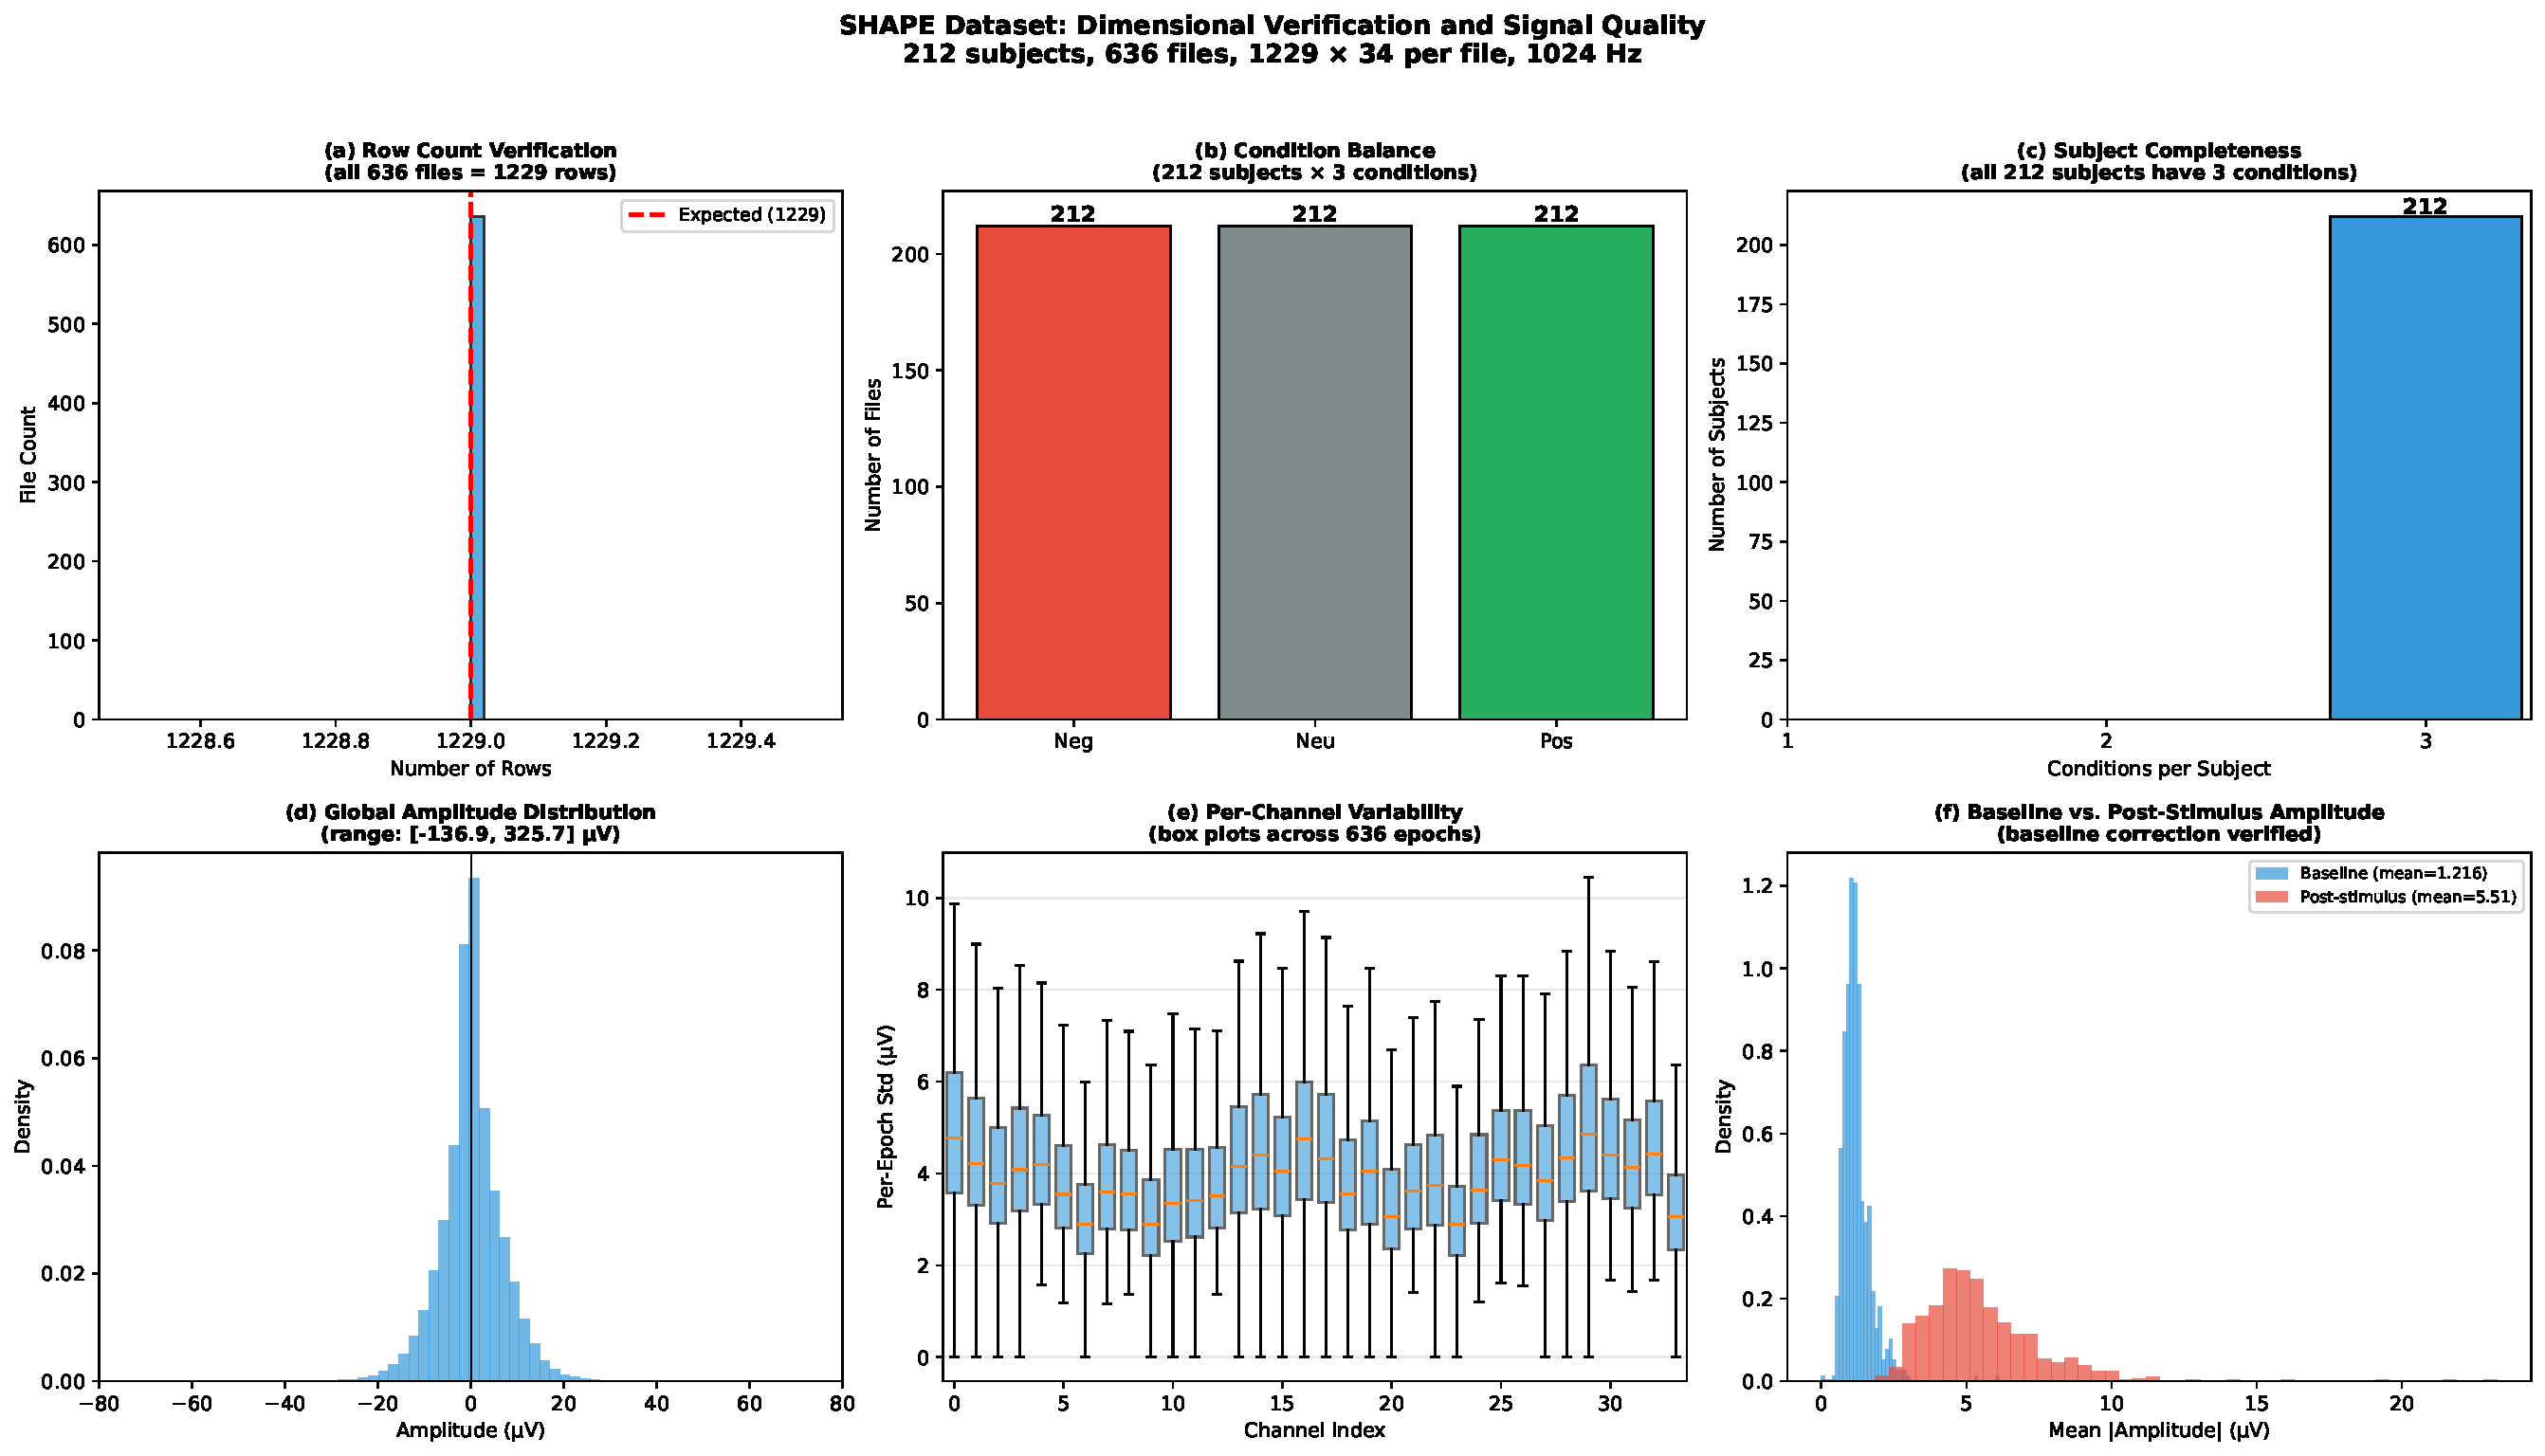
\includegraphics[width=\textwidth]{pictures/chGraphNeuralNetworks/fig_qc_dimensional_verification.pdf}
    \caption{Data verification across $636$ files. (a)~Row counts. (b)~Condition balance. (c)~Subject completeness. (d)~Global amplitude distribution. (e)~Per-channel variability. (f)~Baseline vs.\ post-stimulus amplitude.}
    \label{fig:qc_verification}
\end{figure}

\begin{figure}[H]
    \centering
    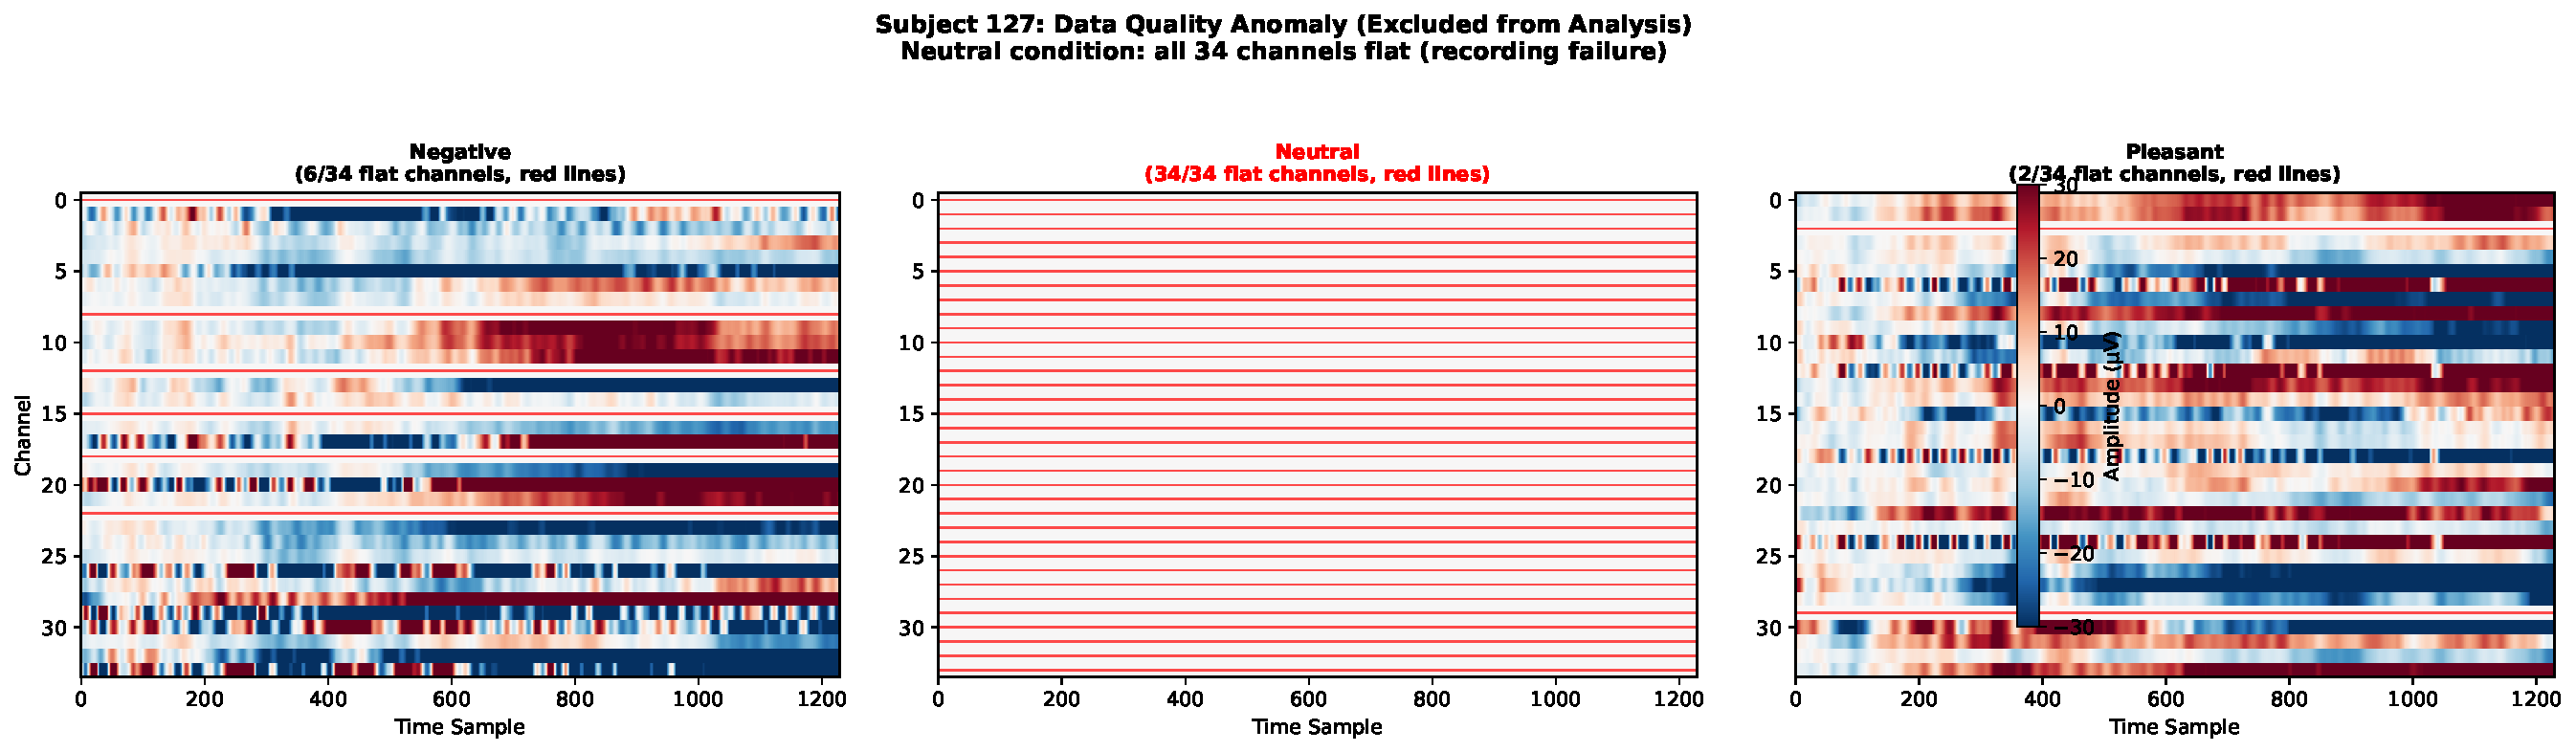
\includegraphics[width=\textwidth]{pictures/chGraphNeuralNetworks/fig_qc_subject127_anomaly.pdf}
    \caption{Subject~$127$ recording anomaly. The Neutral condition is entirely flat across all $34$ channels. Red lines indicate flat channels. This subject was excluded from all analyses.}
    \label{fig:qc_subject127}
\end{figure}

The final dataset comprises $\mathbf{211}$ \textbf{subjects} $\times$ $\mathbf{3}$ \textbf{conditions} $= \mathbf{633}$ \textbf{observations}.

\subsection{Clinical Metadata}

The clinical metadata include $142$ participants with Major Depressive Disorder ($67.3\%$), $82$ with PTSD ($38.9\%$), $85$ with Substance Use Disorder ($40.3\%$), $60$ with GAD ($28.4\%$), $50$ with ADHD ($23.7\%$), $69$ with eating disorders ($32.7\%$), $34$ with mania ($16.1\%$), and $91$ taking psychiatric medication ($43.1\%$). Sex was recorded as female for $172$ participants and male for $33$; six records were unavailable or not represented in those two counts. Mean comorbidity burden is $2.8$ diagnoses per subject (range $0$--$7$).

\begin{figure}[H]
    \centering
    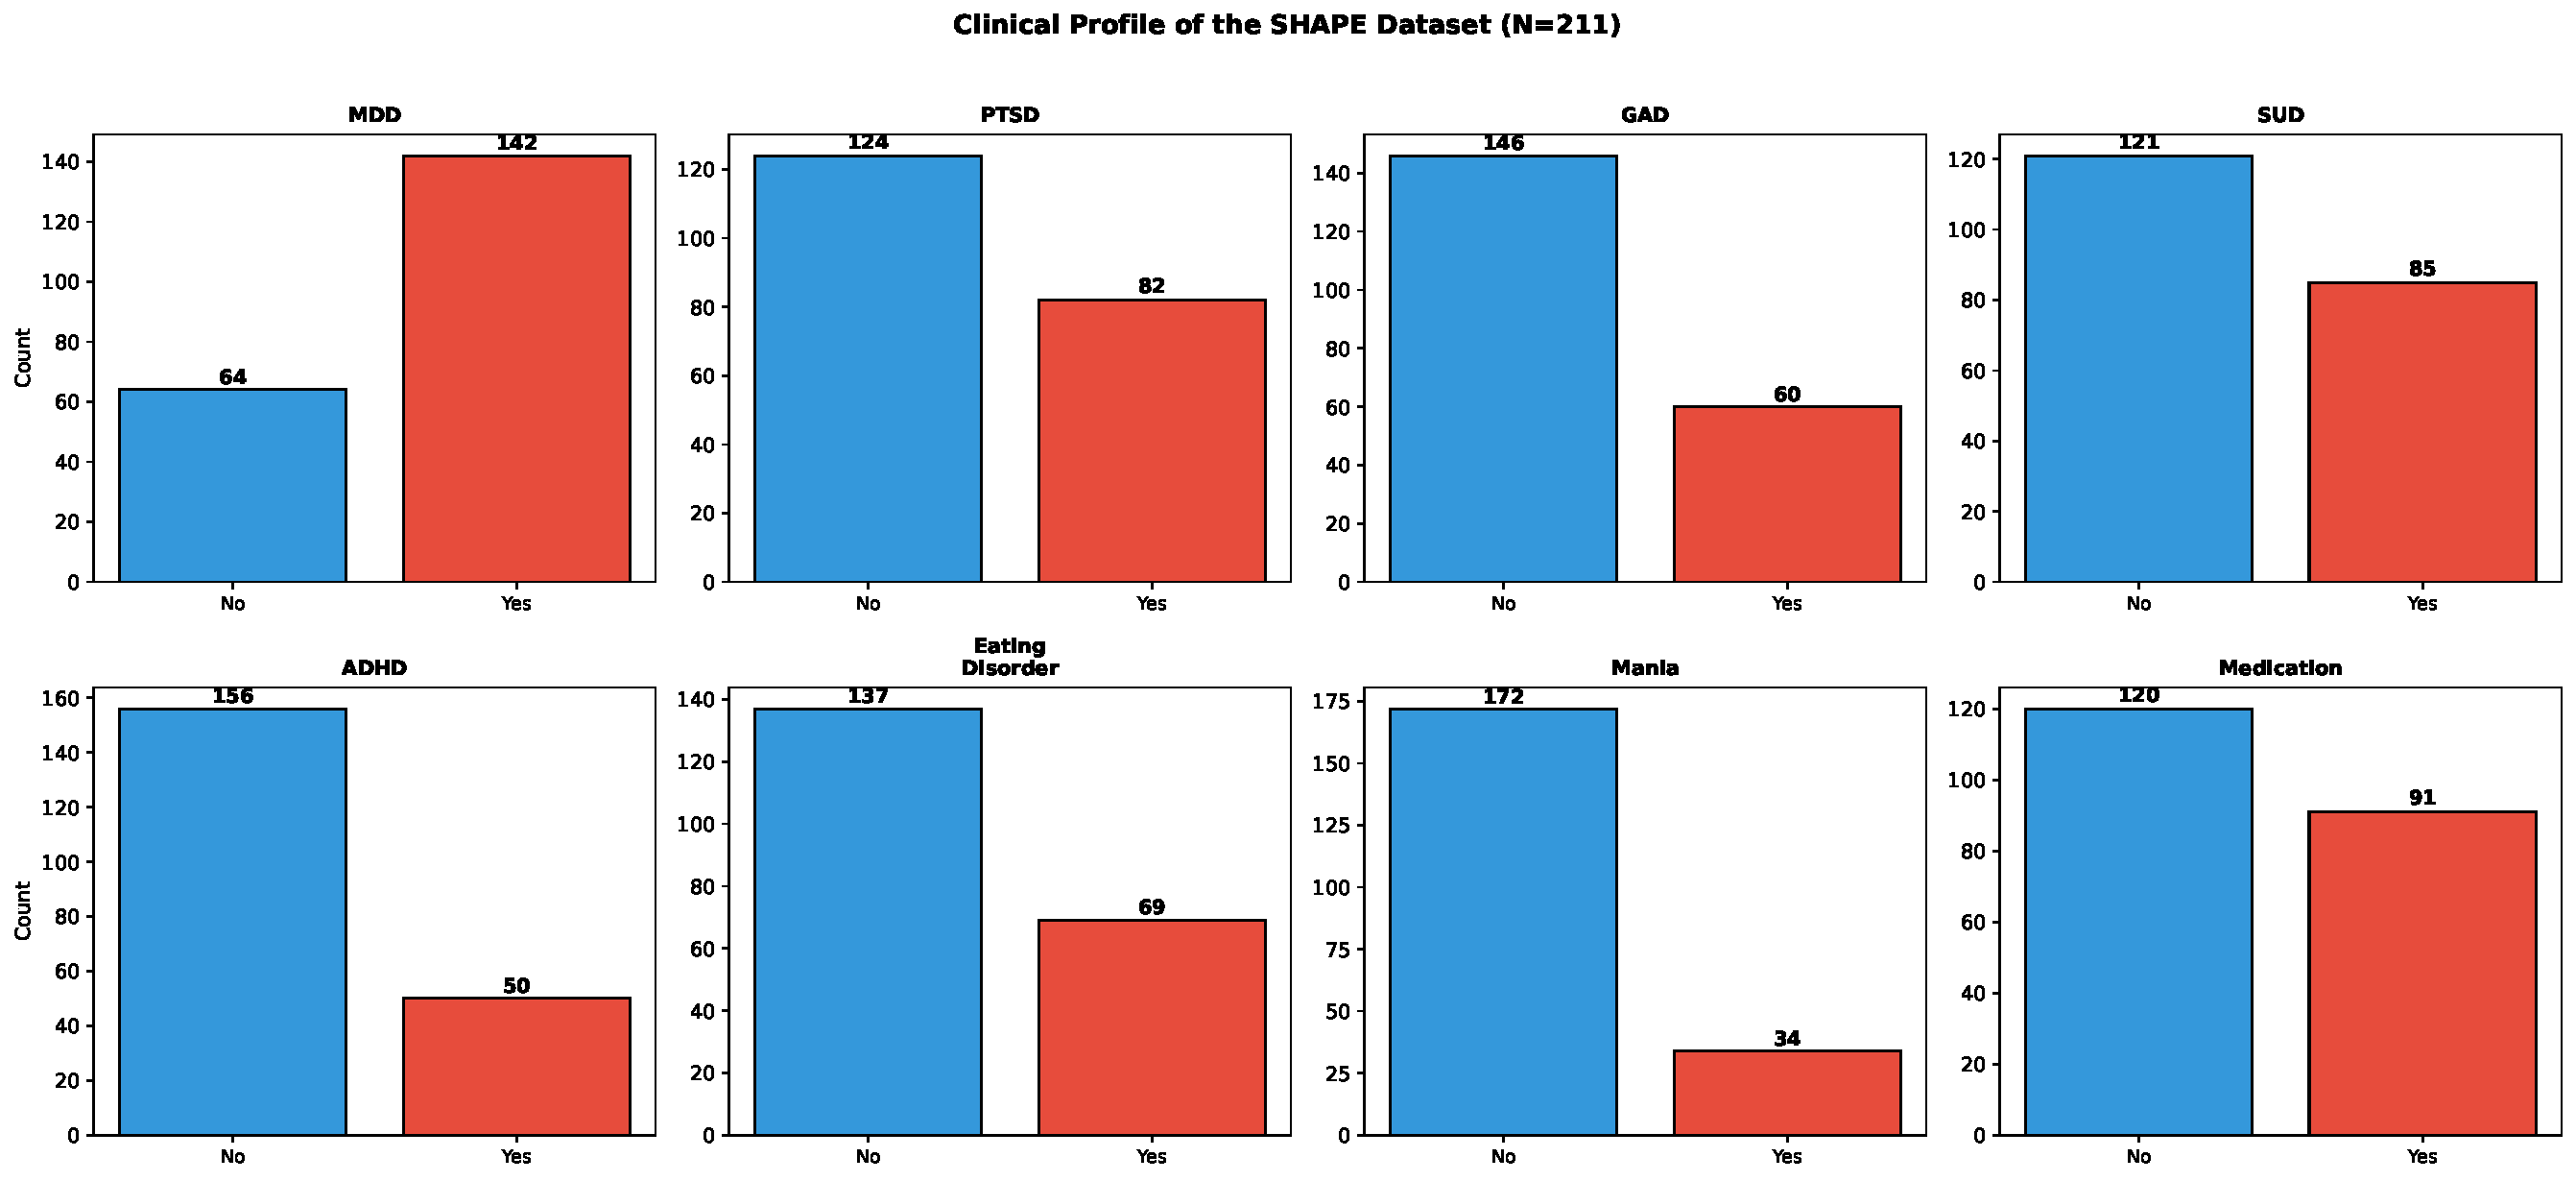
\includegraphics[width=\textwidth]{pictures/chGraphNeuralNetworks/fig_clinical_profile_211.pdf}
    \caption{Clinical profile of the $211$ SHAPE subjects. Eight diagnostic variables with group sizes.}
    \label{fig:clinical_profile}
\end{figure}

\subsection{Preprocessing Pipeline}

Four steps transform each $1229 \times 34$ trial-averaged ERP matrix into the reservoir format: removal of the first $205$ rows, $4\times$ anti-aliasing decimation to $256$~Hz ($256$ post-baseline samples), per-channel z-score normalization, and reservoir processing ($N_{\text{res}}=256$, $\beta=0.05$, $M_{\text{th}}=0.5$). The archived primary extractor divided all 256 samples into six 42-sample bins and omitted the four-sample remainder. That full-epoch BSC$_6$ differs from the steps 10--70 early-window specification in Chapter~\ref{chap:embeddings} and from the later attention analysis. The corrected code uses the stated early window and fits a common PCA-64 basis only on each training fold. The raw inputs were unavailable for rerunning it, so the numerical results below retain the archived full-epoch encoding and global PCA unless explicitly identified as the separate early-window analysis.


\section{Raw Data Observations}
\label{sec:ch5_raw_obs}

Before classification and clinical analysis, this section records summaries at each pipeline stage: z-scored trial-averaged EEG, reservoir spikes, the archived PCA-64 geometry, channel-feature similarity, and variation in the thresholded graphs. The figures are descriptive and inherit the preprocessing limitations stated above.

\subsection{Multichannel EEG Entering the Graph Stage}

The preprocessed dataset provides $633$ condition-level observations ($211$ participants $\times$ $3$ conditions), each a $256 \times 34$ matrix of z-scored amplitudes at $256$~Hz. Figure~\ref{fig:obs01_eeg} displays three selected participants. After per-channel z-scoring, the pooled distribution is centered at $0.000$ with unit variance and a range of $[-5.41, 5.01]$. Waveform morphology differs across the displayed participants. Because each participant contributes three rows, all predictive splits must keep a participant's rows together.

\begin{figure}[H]
    \centering
    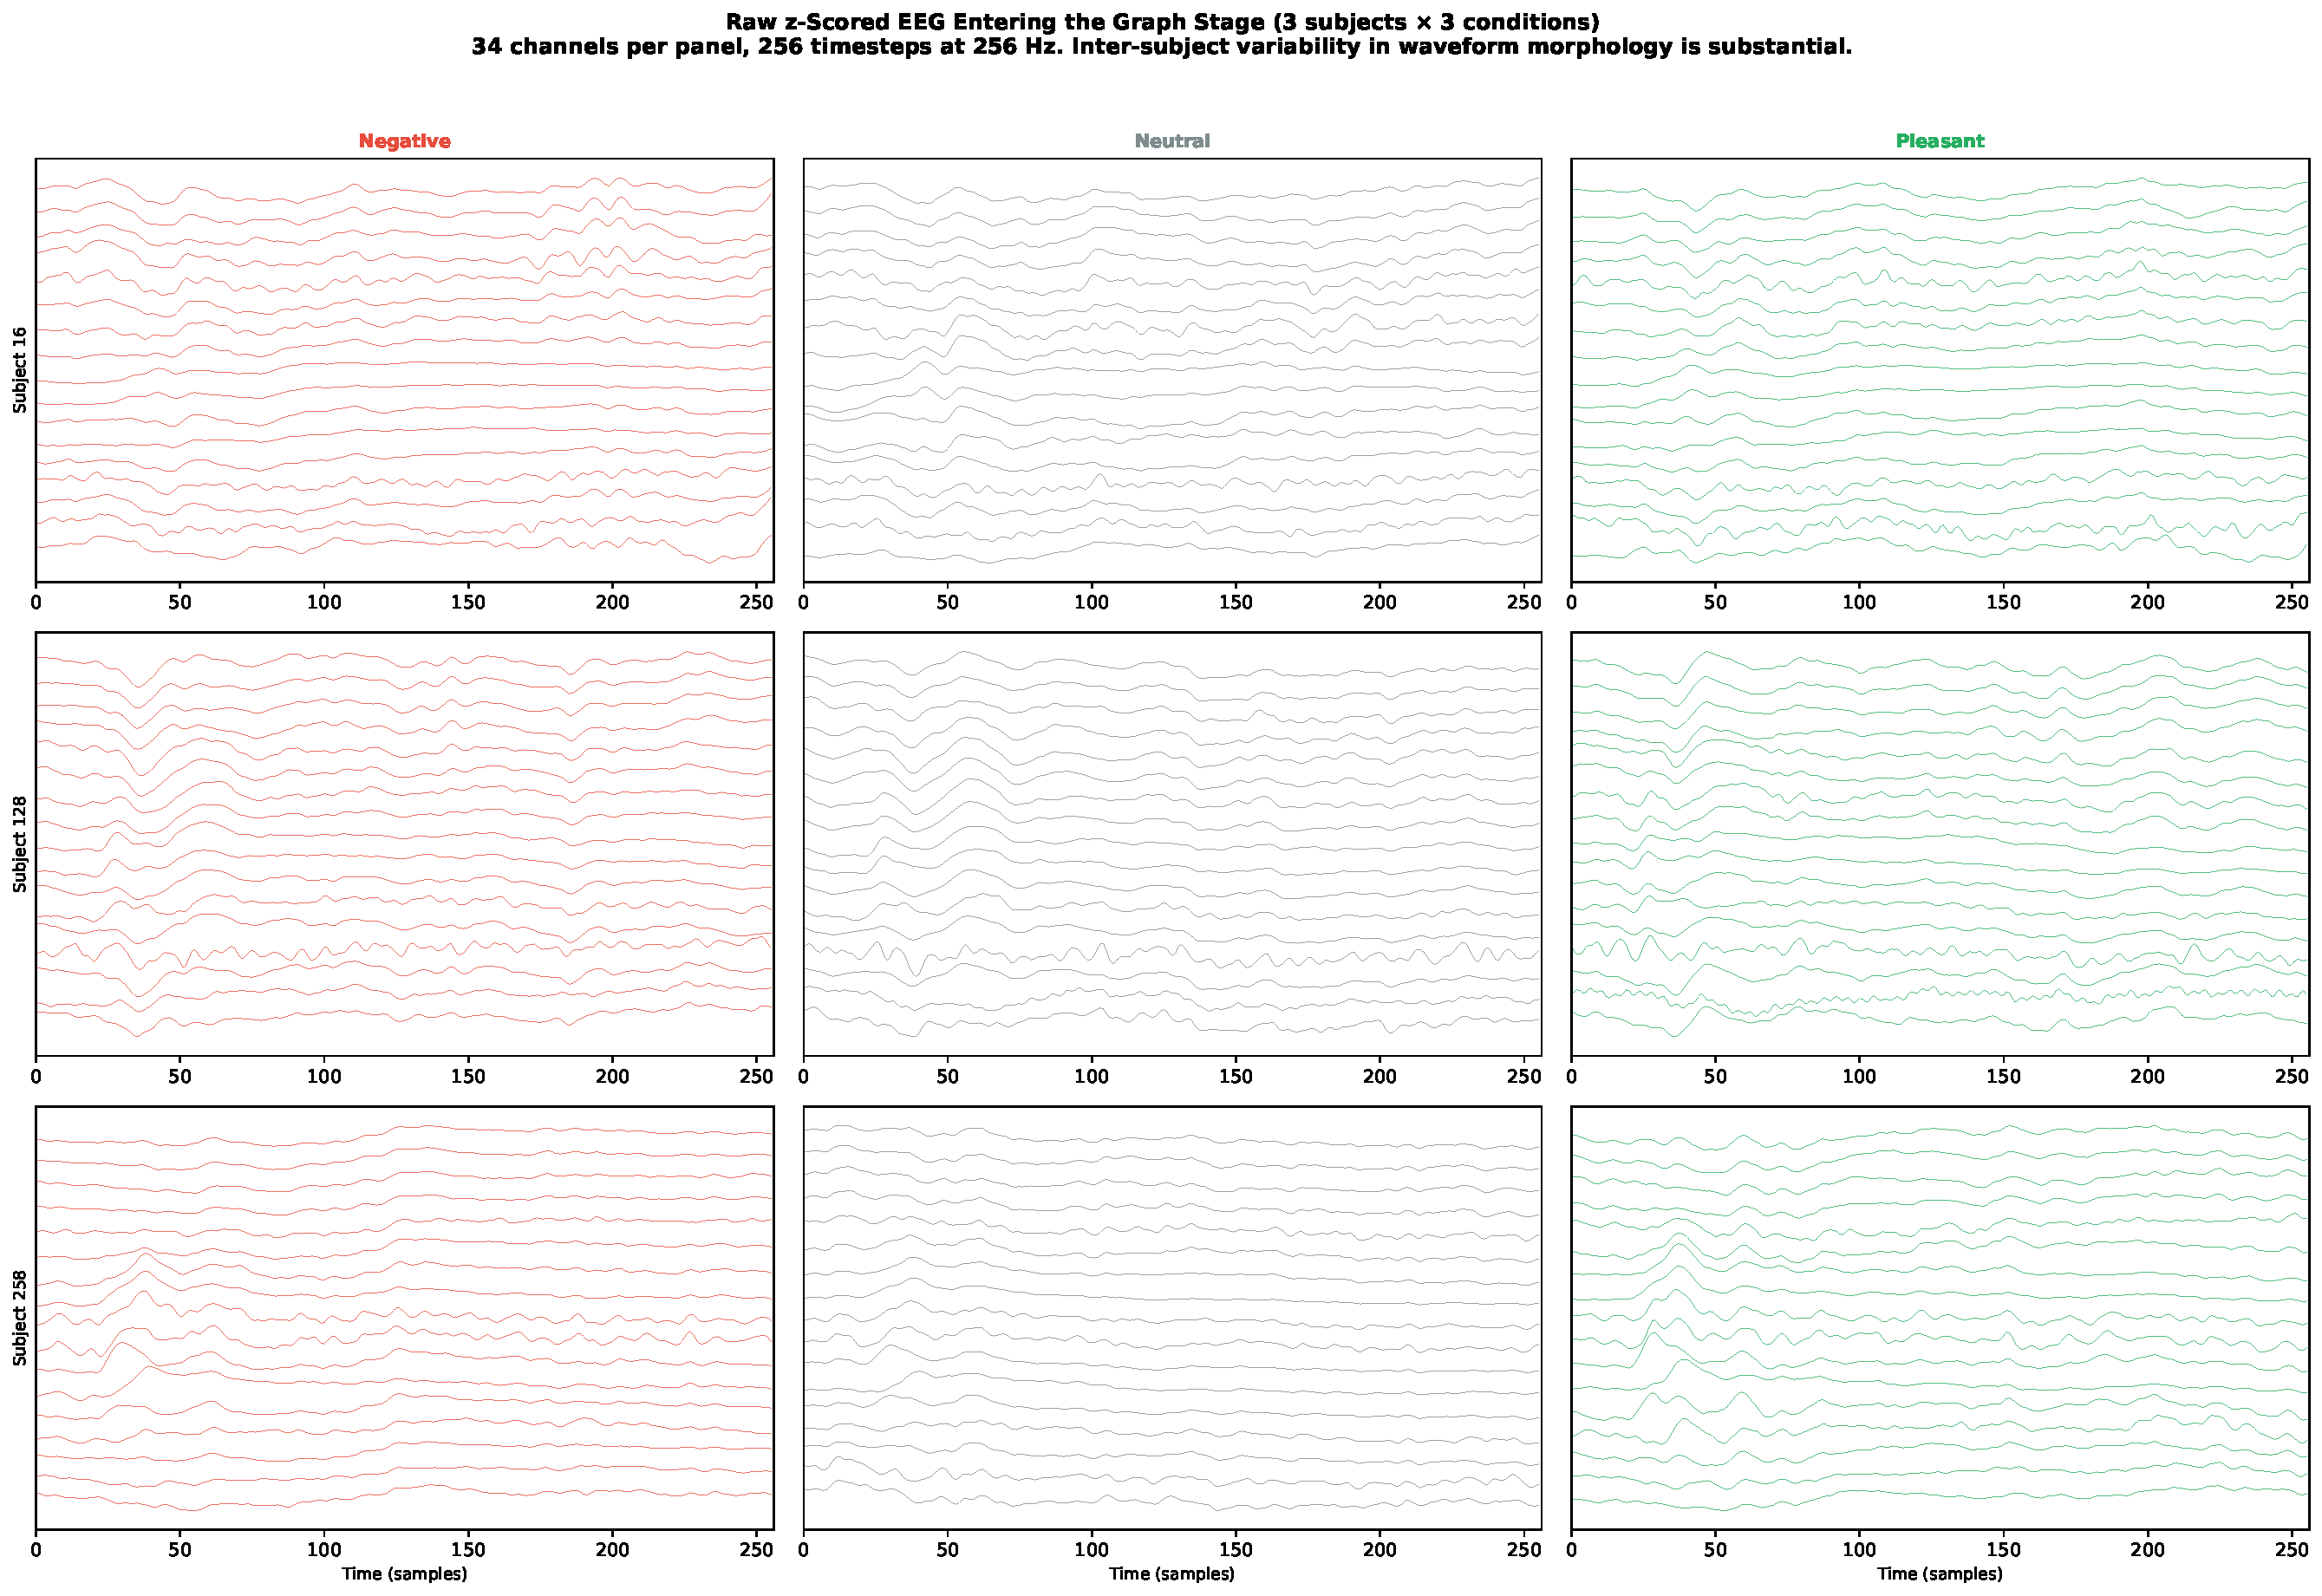
\includegraphics[width=\textwidth]{pictures/chGraphNeuralNetworks/obs01_raw_eeg_waveforms.pdf}
    \caption{Selected z-scored, trial-averaged EEG inputs ($3$ participants $\times$ $3$ conditions). Each panel shows $17$ of $34$ channels offset vertically over $256$ time steps. The examples illustrate both between-participant and within-participant differences but do not estimate their population ratio.}
    \label{fig:obs01_eeg}
\end{figure}

\subsection{Reservoir Spike Response on Real EEG}

Figure~\ref{fig:obs02_spikes} shows the reservoir response for one selected participant under all three conditions. The top row contains spike rasters for Channel~10, and the bottom row contains population firing-rate traces for four channels. Across the full SHAPE feature array, $47.4\%$ of BSC$_6$ entries are zero, compared with $79.1\%$ for the synthetic generator. The mean entry is $5.15$, and the maximum is $42$ spikes per neuron per bin. These values describe the different input distributions; they do not isolate why their sparsity differs.

\begin{figure}[H]
    \centering
    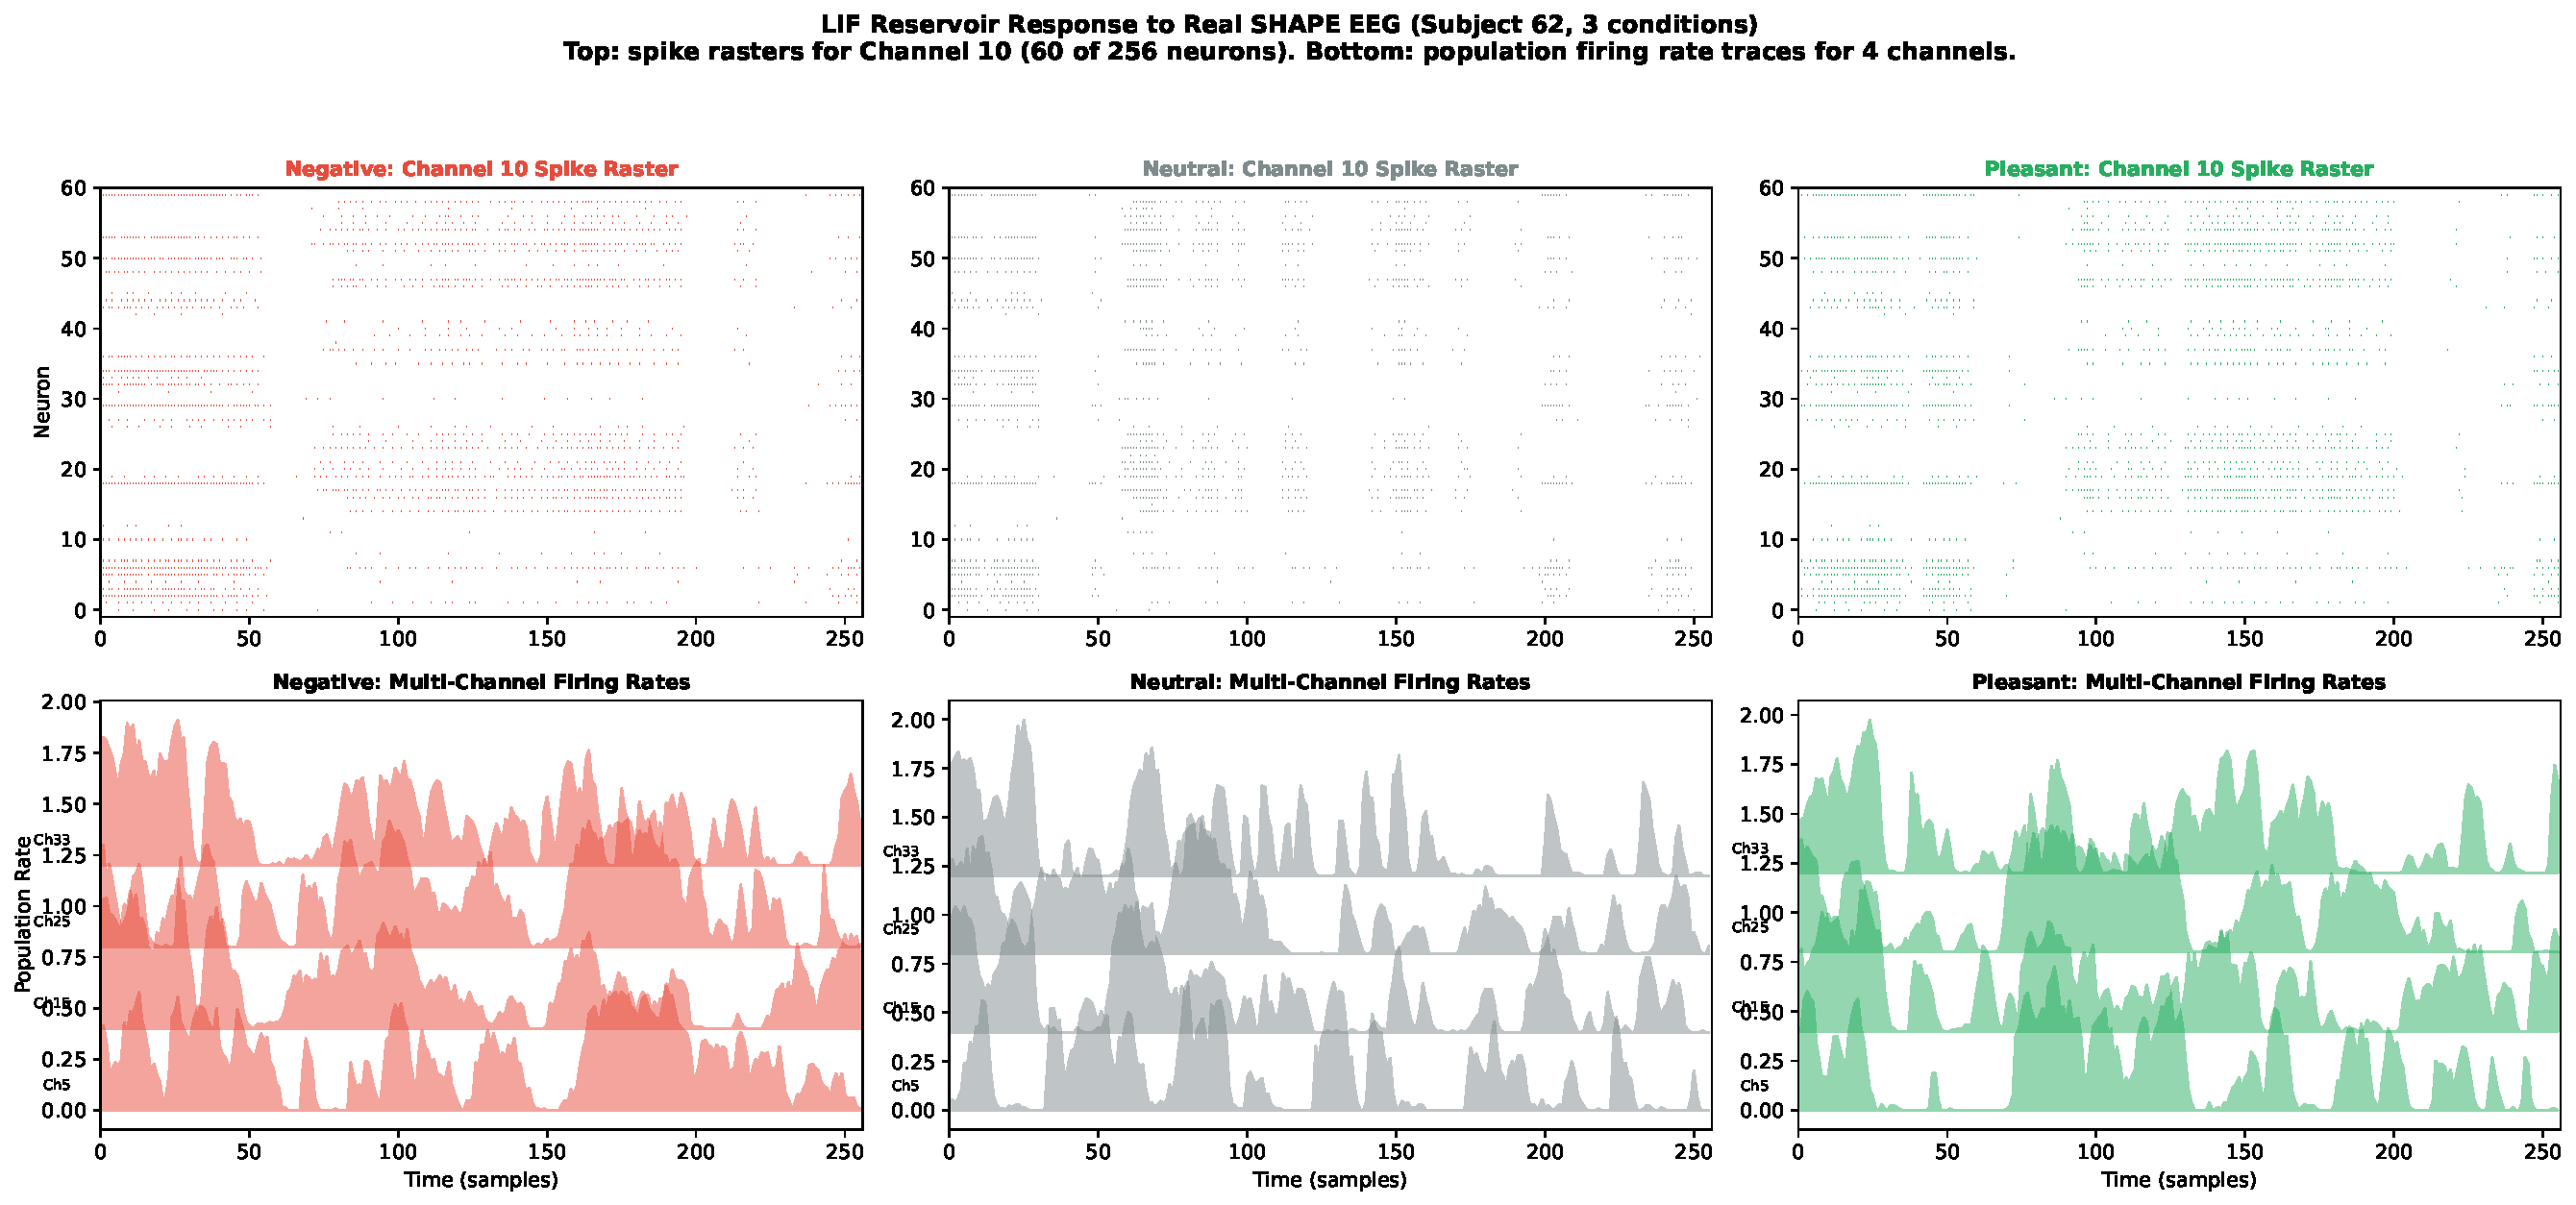
\includegraphics[width=\textwidth]{pictures/chGraphNeuralNetworks/obs02_raw_spike_trains.pdf}
    \caption{Reservoir response to SHAPE EEG for one participant and three conditions. Top: spike rasters for Channel~10 ($60$ of $256$ units). Bottom: population firing-rate traces for four channel indices.}
    \label{fig:obs02_spikes}
\end{figure}

\subsection{PCA-64 Embedding Geometry}

Figure~\ref{fig:obs03_embeddings} characterizes the archived PCA-64 embedding space. The left panel projects the concatenated $34 \times 64 = 2{,}176$-dimensional embeddings into two dimensions, colored by emotional condition; the conditions overlap substantially. The center panel colors the same projection by subject identity and shows tighter within-subject grouping. The right panel shows per-channel embedding variance, ranging from $36{,}900$ (Channel~16) to $70{,}721$ (Channel~29), with a coefficient of variation of $0.15$. These are in-sample geometric summaries of the global-PCA representation and should not be read as held-out evidence.

\begin{figure}[H]
    \centering
    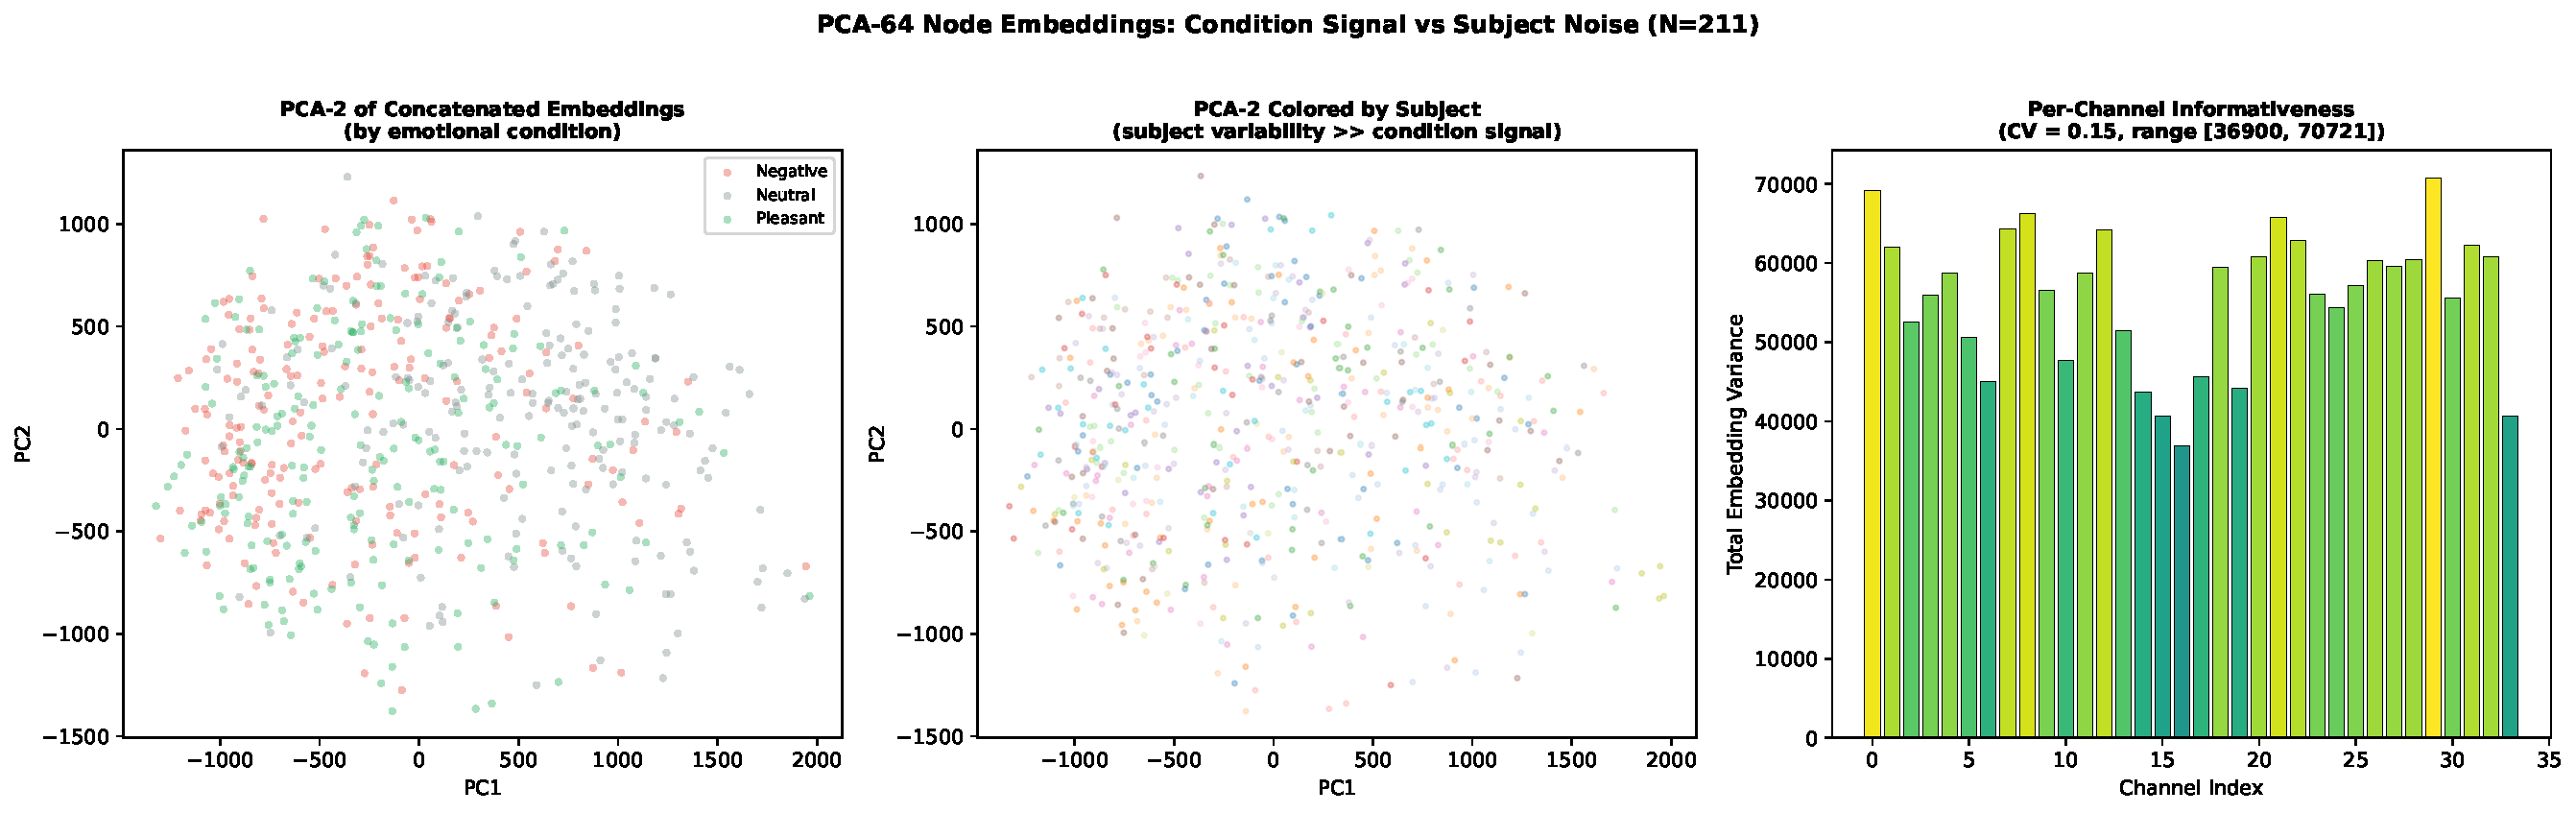
\includegraphics[width=\textwidth]{pictures/chGraphNeuralNetworks/obs03_bsc6_pca64_embeddings.pdf}
    \caption{Archived PCA-64 embedding geometry ($N = 211$). Left: PCA-2 by condition. Center: PCA-2 by subject. Right: per-channel embedding variance. PCA was fitted globally for this descriptive figure.}
    \label{fig:obs03_embeddings}
\end{figure}

\subsection{Archived Inter-Channel Feature Similarity}

Figure~\ref{fig:obs04_connectivity} displays the archived correlations between per-channel PCA coordinate vectors and the resulting thresholded graphs. The mean displayed correlation is $\bar{r}=0.143$ (SD $0.552$). Because each channel's PCA basis was fitted separately, coordinate positions do not have a shared meaning across channels. These values describe the archived numerical construction only and are not estimates of EEG channel connectivity.

At the fixed $20\%$ density threshold, each condition-average graph contains $113$ edges, with mean degree $6.6$. Terms such as ``hub,'' ``clustering,'' and ``component'' below refer to this mathematical similarity graph, not to anatomical hubs or communication in a brain network.

\begin{figure}[H]
    \centering
    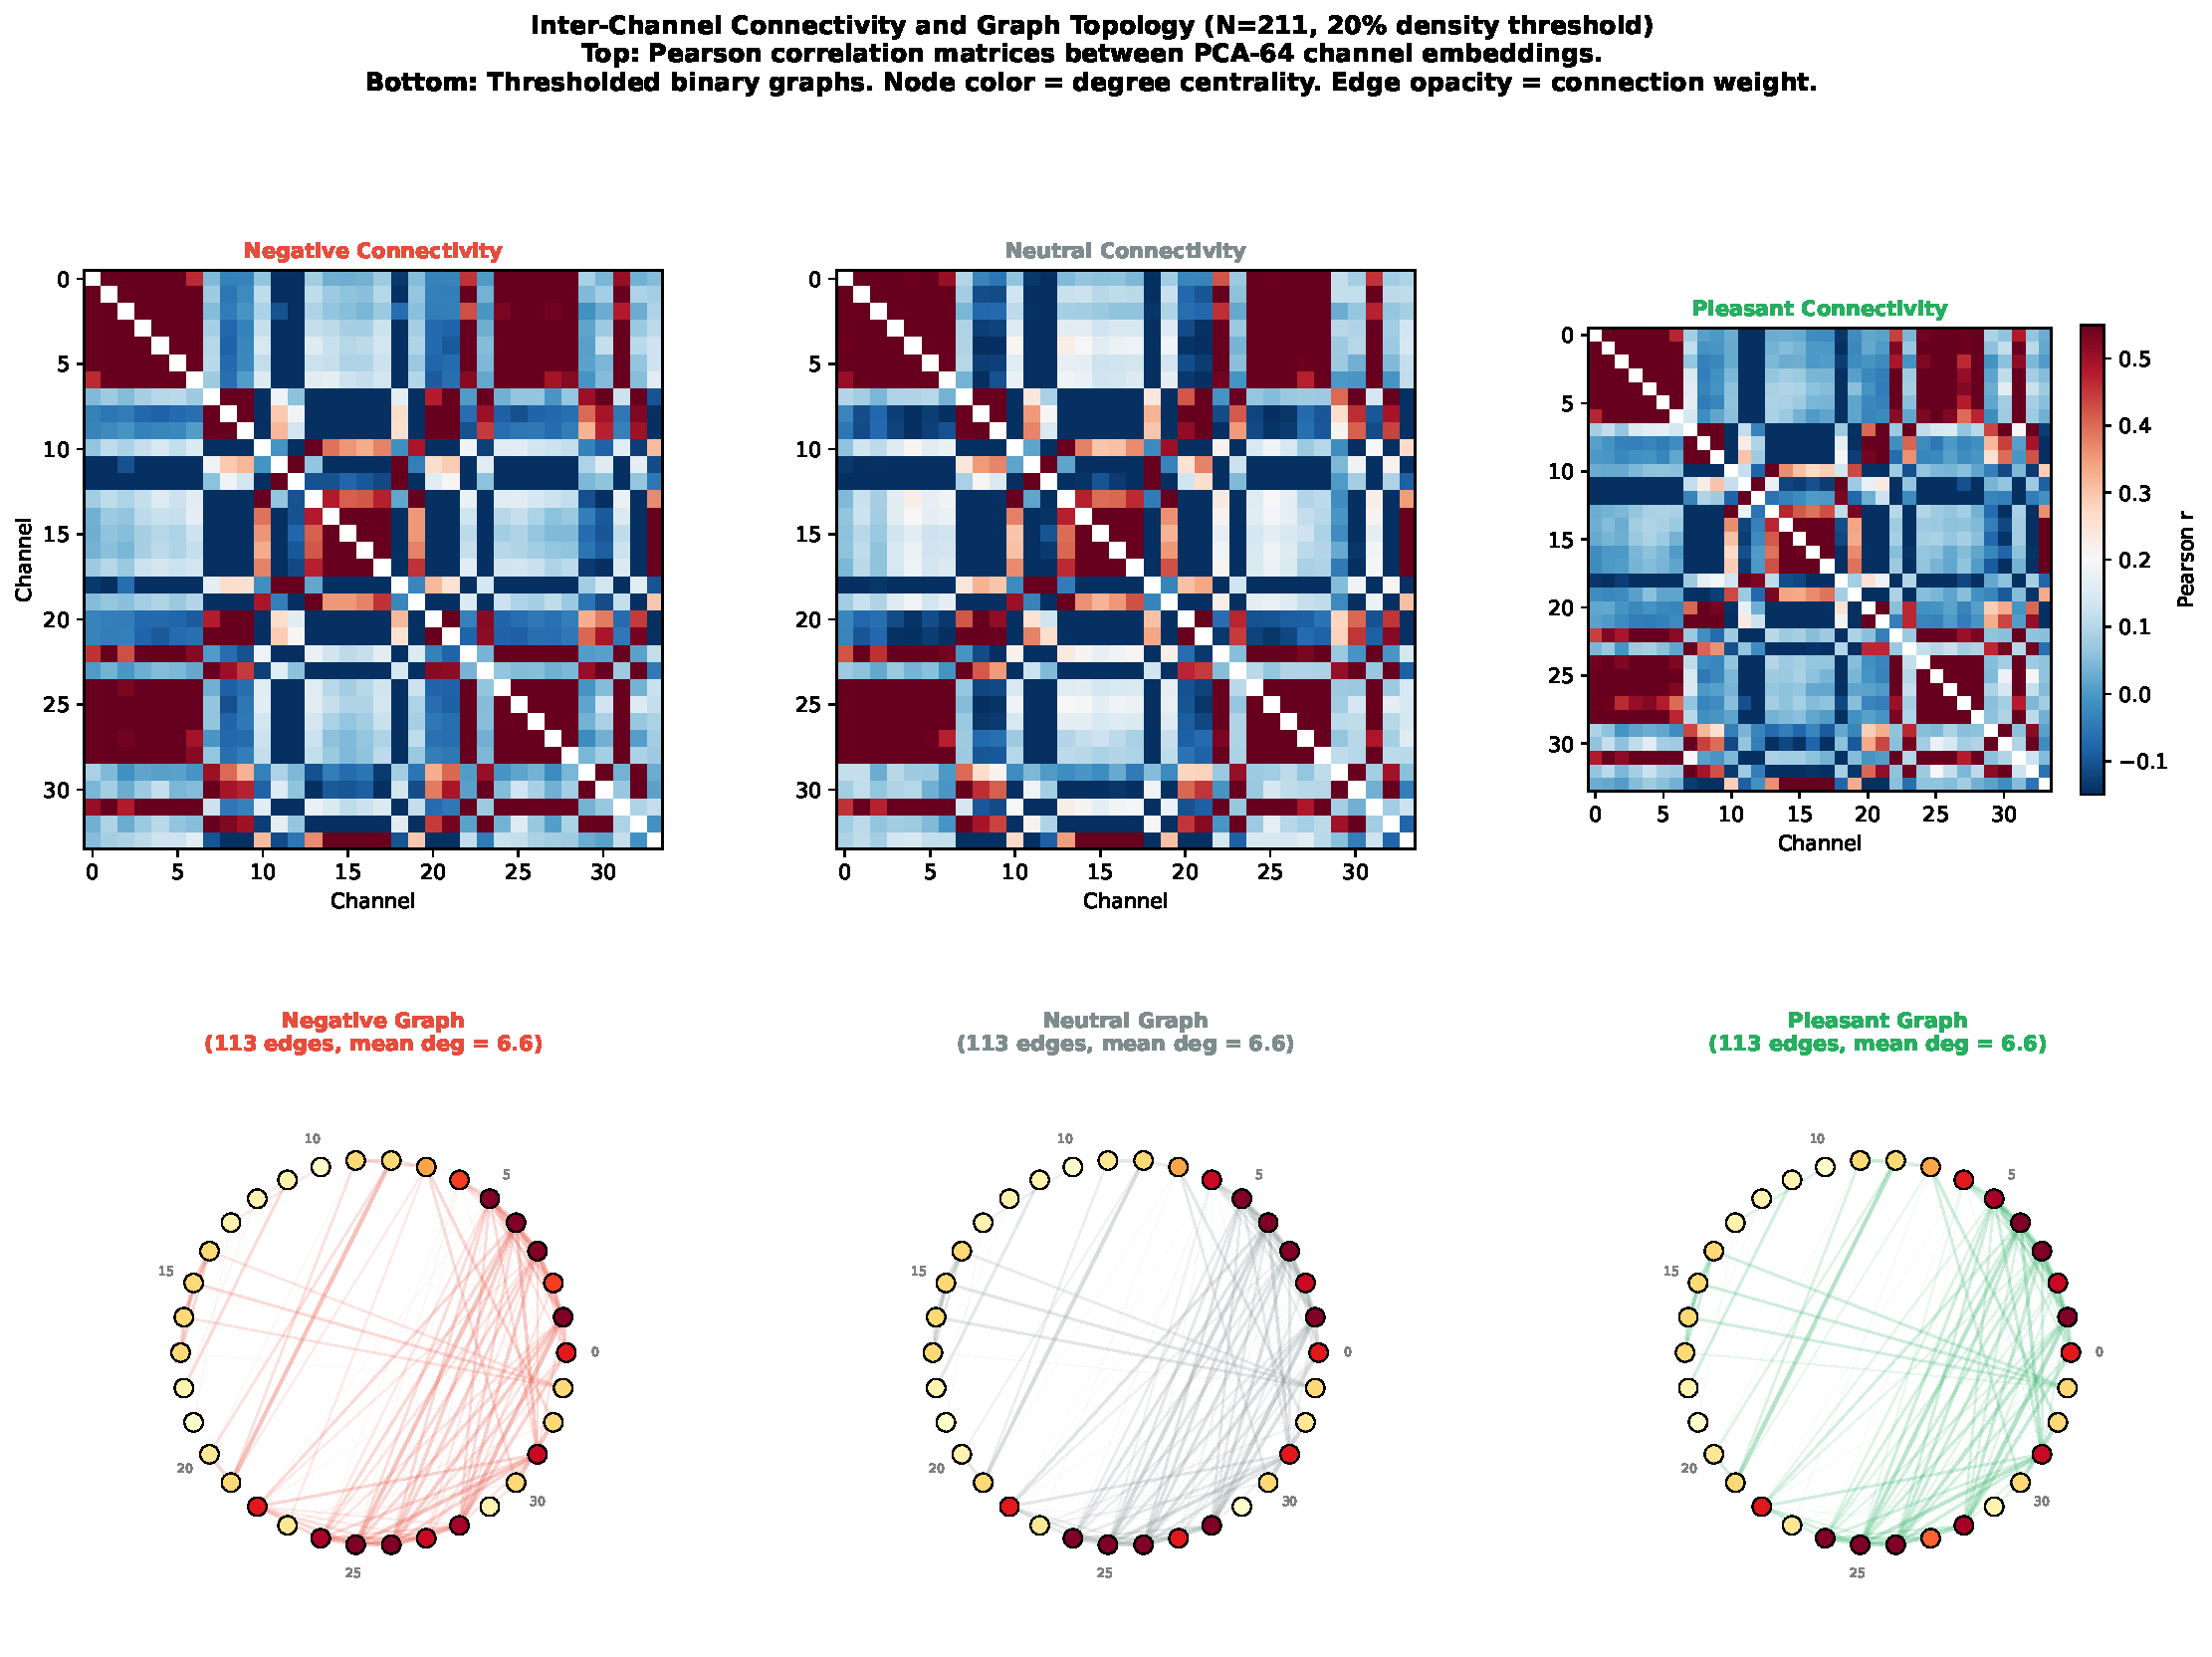
\includegraphics[width=\textwidth]{pictures/chGraphNeuralNetworks/obs04_raw_connectivity_matrices.pdf}
    \caption{Archived cross-channel PCA-coordinate similarity and thresholded graphs ($N=211$, $20\%$ density). Separately fitted channel PCA axes are not commensurate; the figure is retained as a record of the legacy construction and has no physiological-connectivity interpretation.}
    \label{fig:obs04_connectivity}
\end{figure}

\subsection{Between-Subject Graph Variability}

Figure~\ref{fig:obs07_variability} records between-participant variation in the archived graph construction. The selected graphs have different edge and degree patterns under the same $20\%$ density rule. The displayed edge-weight standard deviation is $0.303$, and degrees across participant--channel combinations range from $0$ to $15$ with mean $6.6$.

The Negative-minus-Pleasant panel shows differences in the archived similarity values. Between-subject variability ($\sigma=0.303$) is approximately seven times the mean absolute condition difference ($|\Delta r|=0.045$). This descriptive ratio is not a signal-to-noise estimate and does not establish either a physiological condition signal or inter-individual brain-network organization.

\begin{figure}[H]
    \centering
    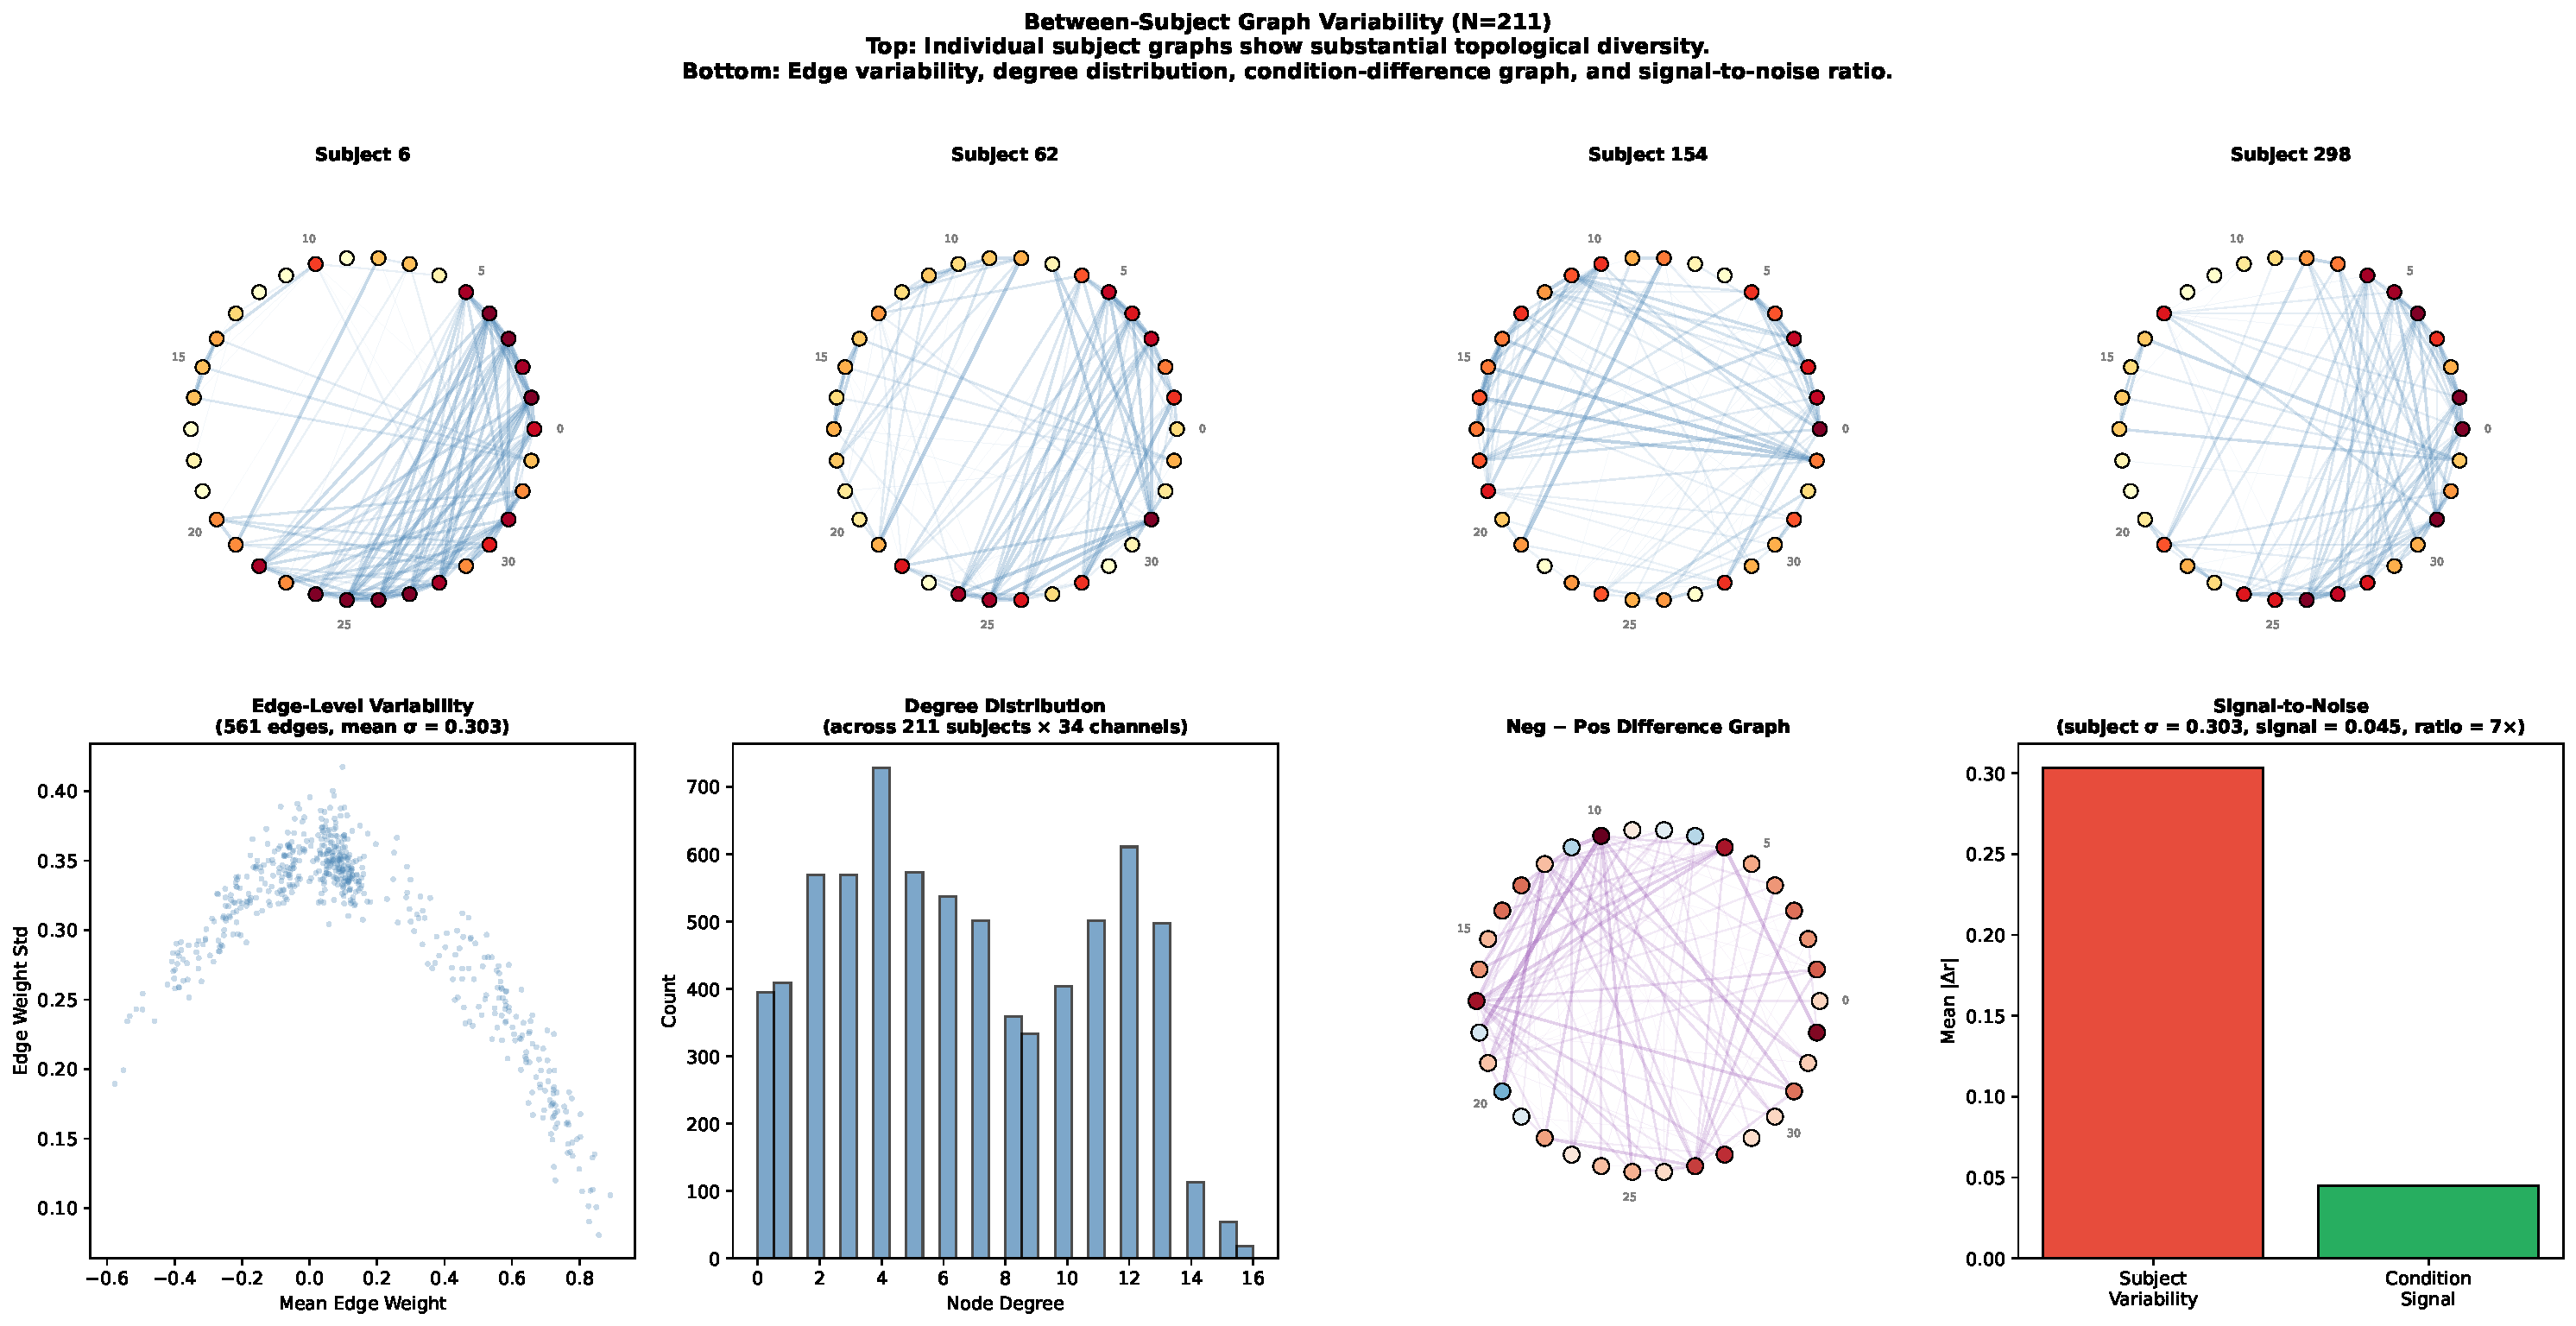
\includegraphics[width=\textwidth]{pictures/chGraphNeuralNetworks/obs07_graph_variability.pdf}
    \caption{Variability of the archived thresholded similarity graphs ($N=211$). The displayed sevenfold ratio compares two summary scales; it is not a formal signal-to-noise ratio.}
    \label{fig:obs07_variability}
\end{figure}

The descriptive figures show substantial between-subject variation, overlapping condition projections, and broad archived similarity values. Because of the global and noncommensurate PCA construction, these plots should be used to understand the legacy analysis rather than to infer heterophily or physiological network structure.

\subsection{The Reservoir's Spike Representation on Real EEG}

Figure~\ref{fig:obs13_bsc6} characterizes the BSC$_6$ features produced from the trial-averaged SHAPE inputs. Each observation is a $34 \times 256 \times 6$ tensor ($34$ channels, $256$ reservoir units, $6$ temporal bins), yielding $52{,}224$ spike-count features. The array is $47.4\%$ zero, compared with $79.1\%$ for the synthetic task in Chapter~\ref{chap:embeddings}. Nonzero entries have mean $9.79$, median $7$, and maximum $42$ spikes per unit per bin.

\begin{figure}[H]
    \centering
    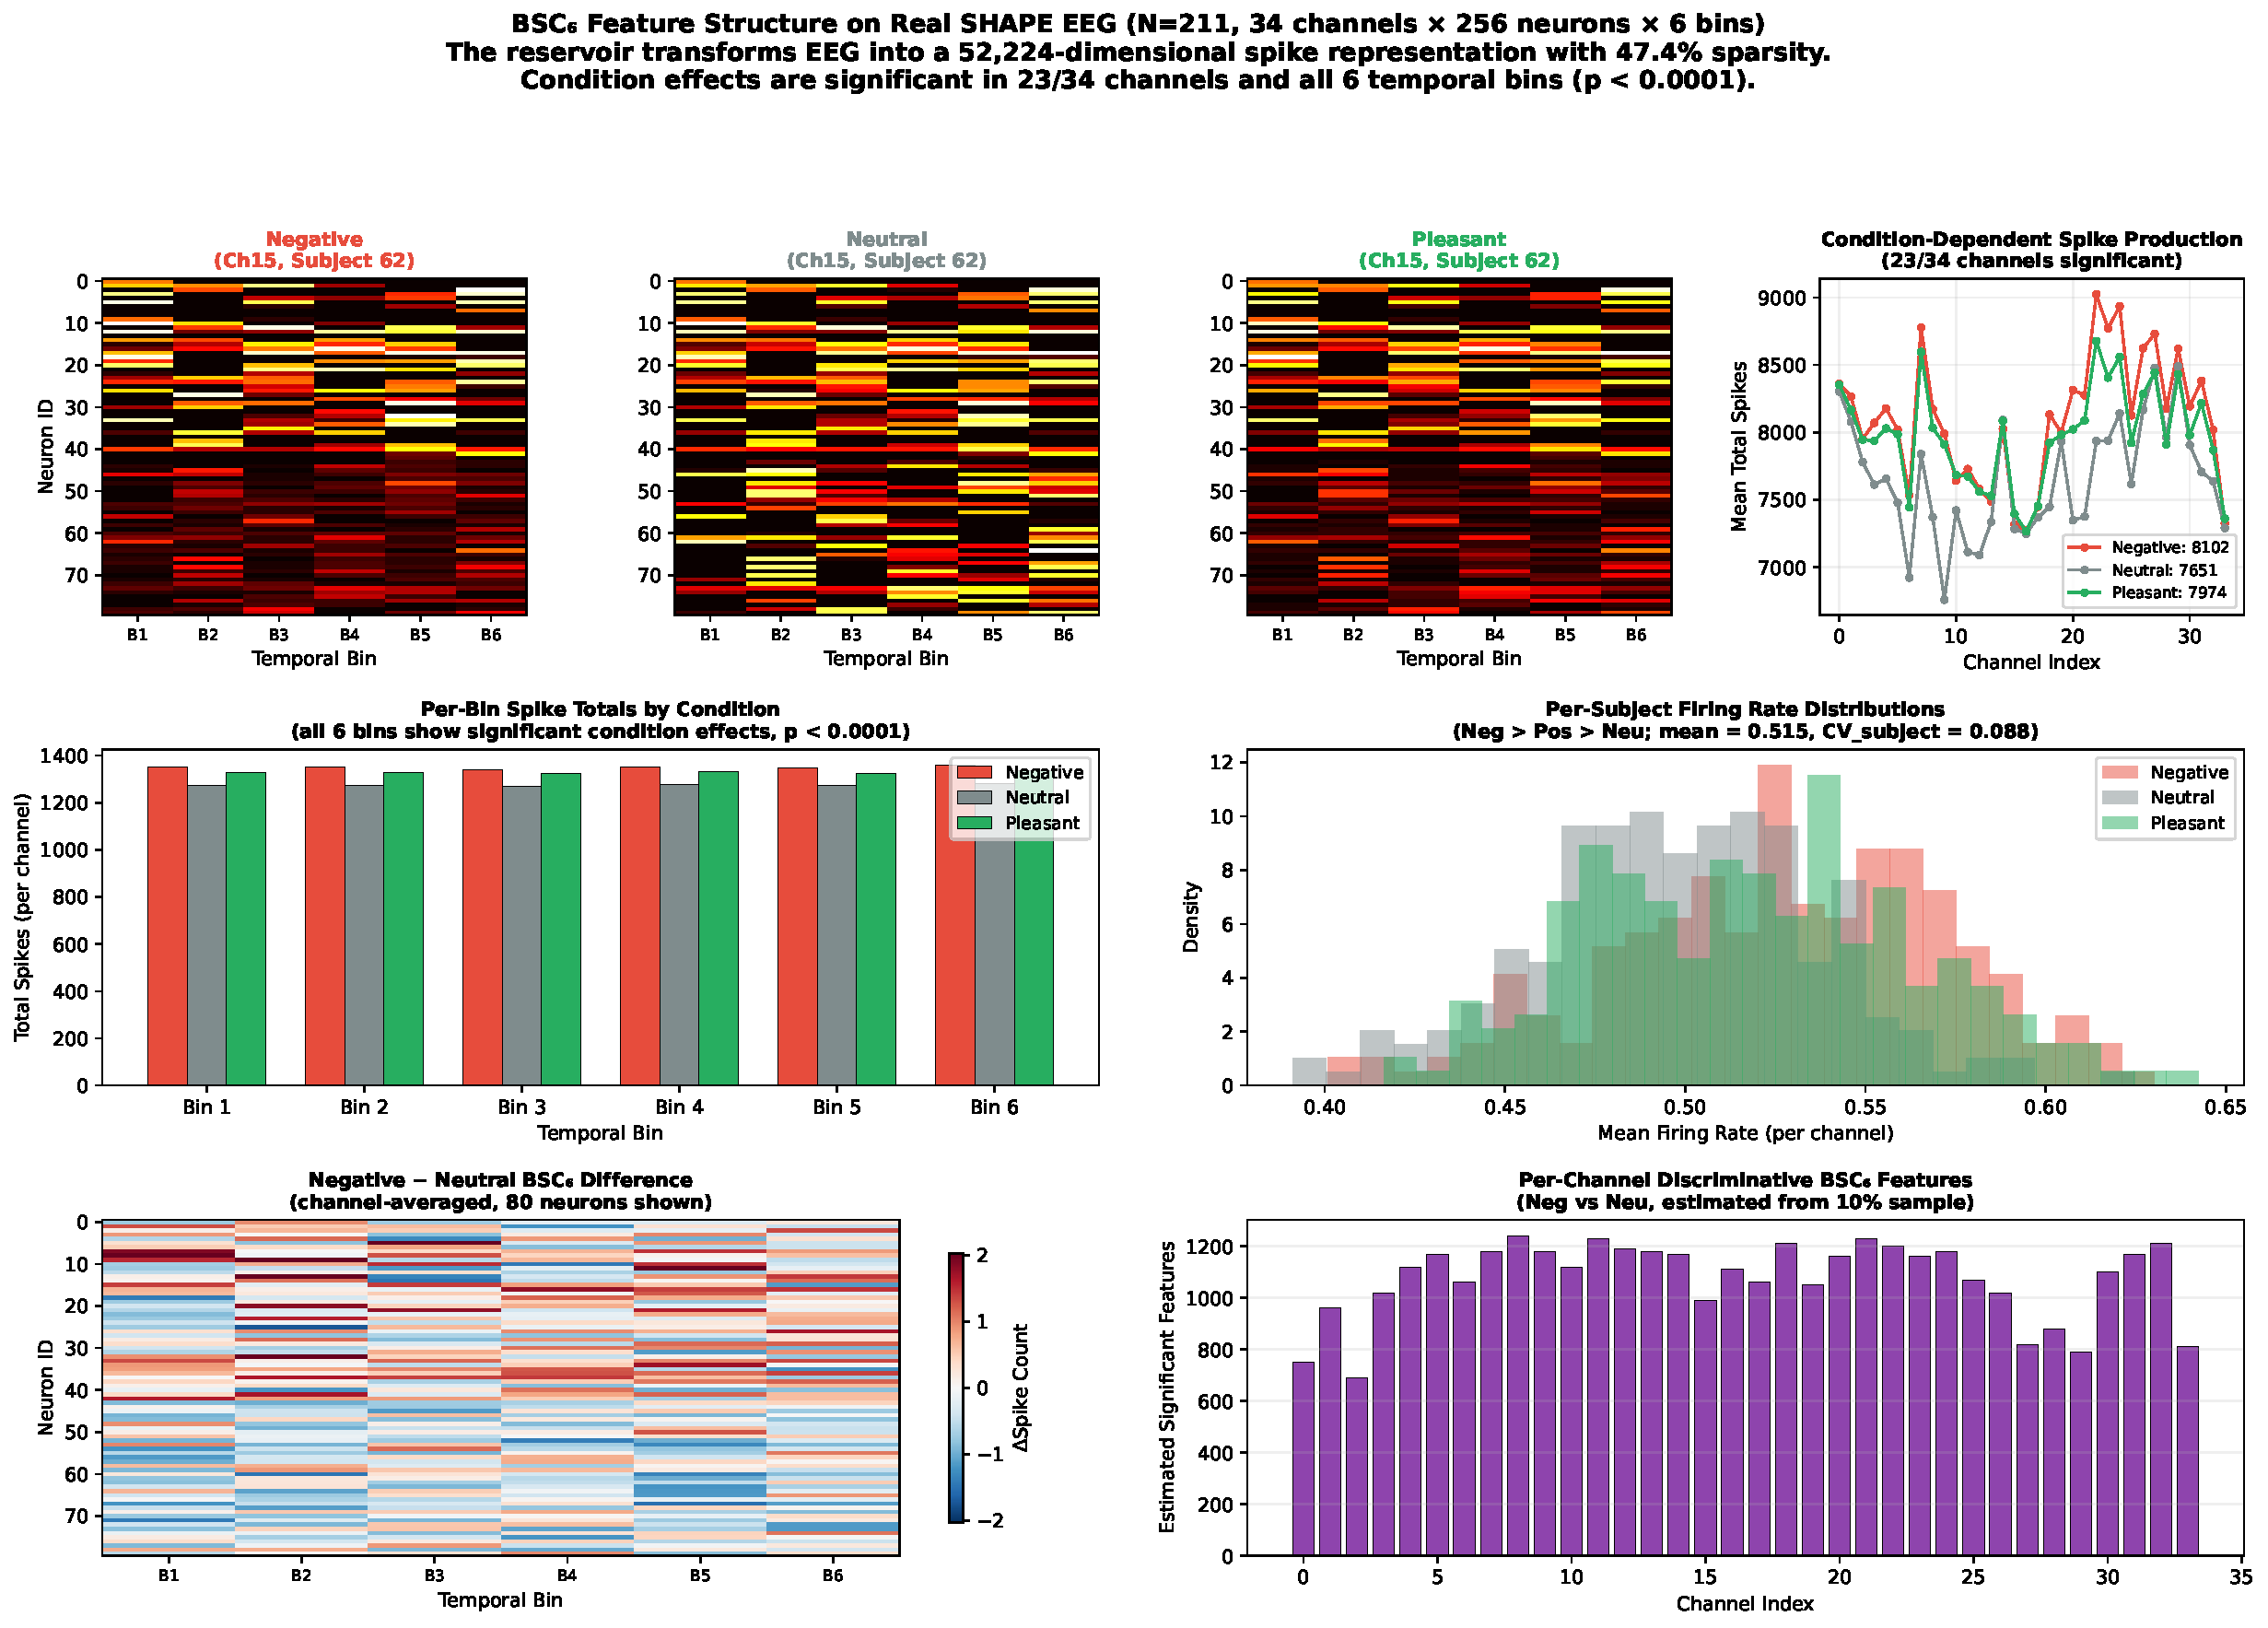
\includegraphics[width=\textwidth]{pictures/chGraphNeuralNetworks/obs13_bsc6_real_eeg.pdf}
    \caption{BSC$_6$ features on SHAPE EEG ($N=211$). The channel and bin $p$ values shown in the archived figure are nominal and were not adjusted as one prespecified family.}
    \label{fig:obs13_bsc6}
\end{figure}

The archived full-epoch summaries are Negative $8{,}102\pm1{,}220$, Neutral $7{,}651\pm1{,}153$, and Pleasant $7{,}974\pm1{,}175$ spikes per channel. Nominal channel and bin tests produce small $p$ values, but the family was not prespecified or multiplicity adjusted. These bins each span 42 samples (about 164~ms) across samples 0--251; four trailing samples are omitted. They must not be interpreted using the 39--273~ms early-window labels reported in the later traceability analysis.

\subsection{Geometry Before and After Panel Centering}

Figure~\ref{fig:obs14_geometry} compares pairwise distances in the archived representation before and after subtracting each participant's three-observation mean.

\begin{figure}[H]
    \centering
    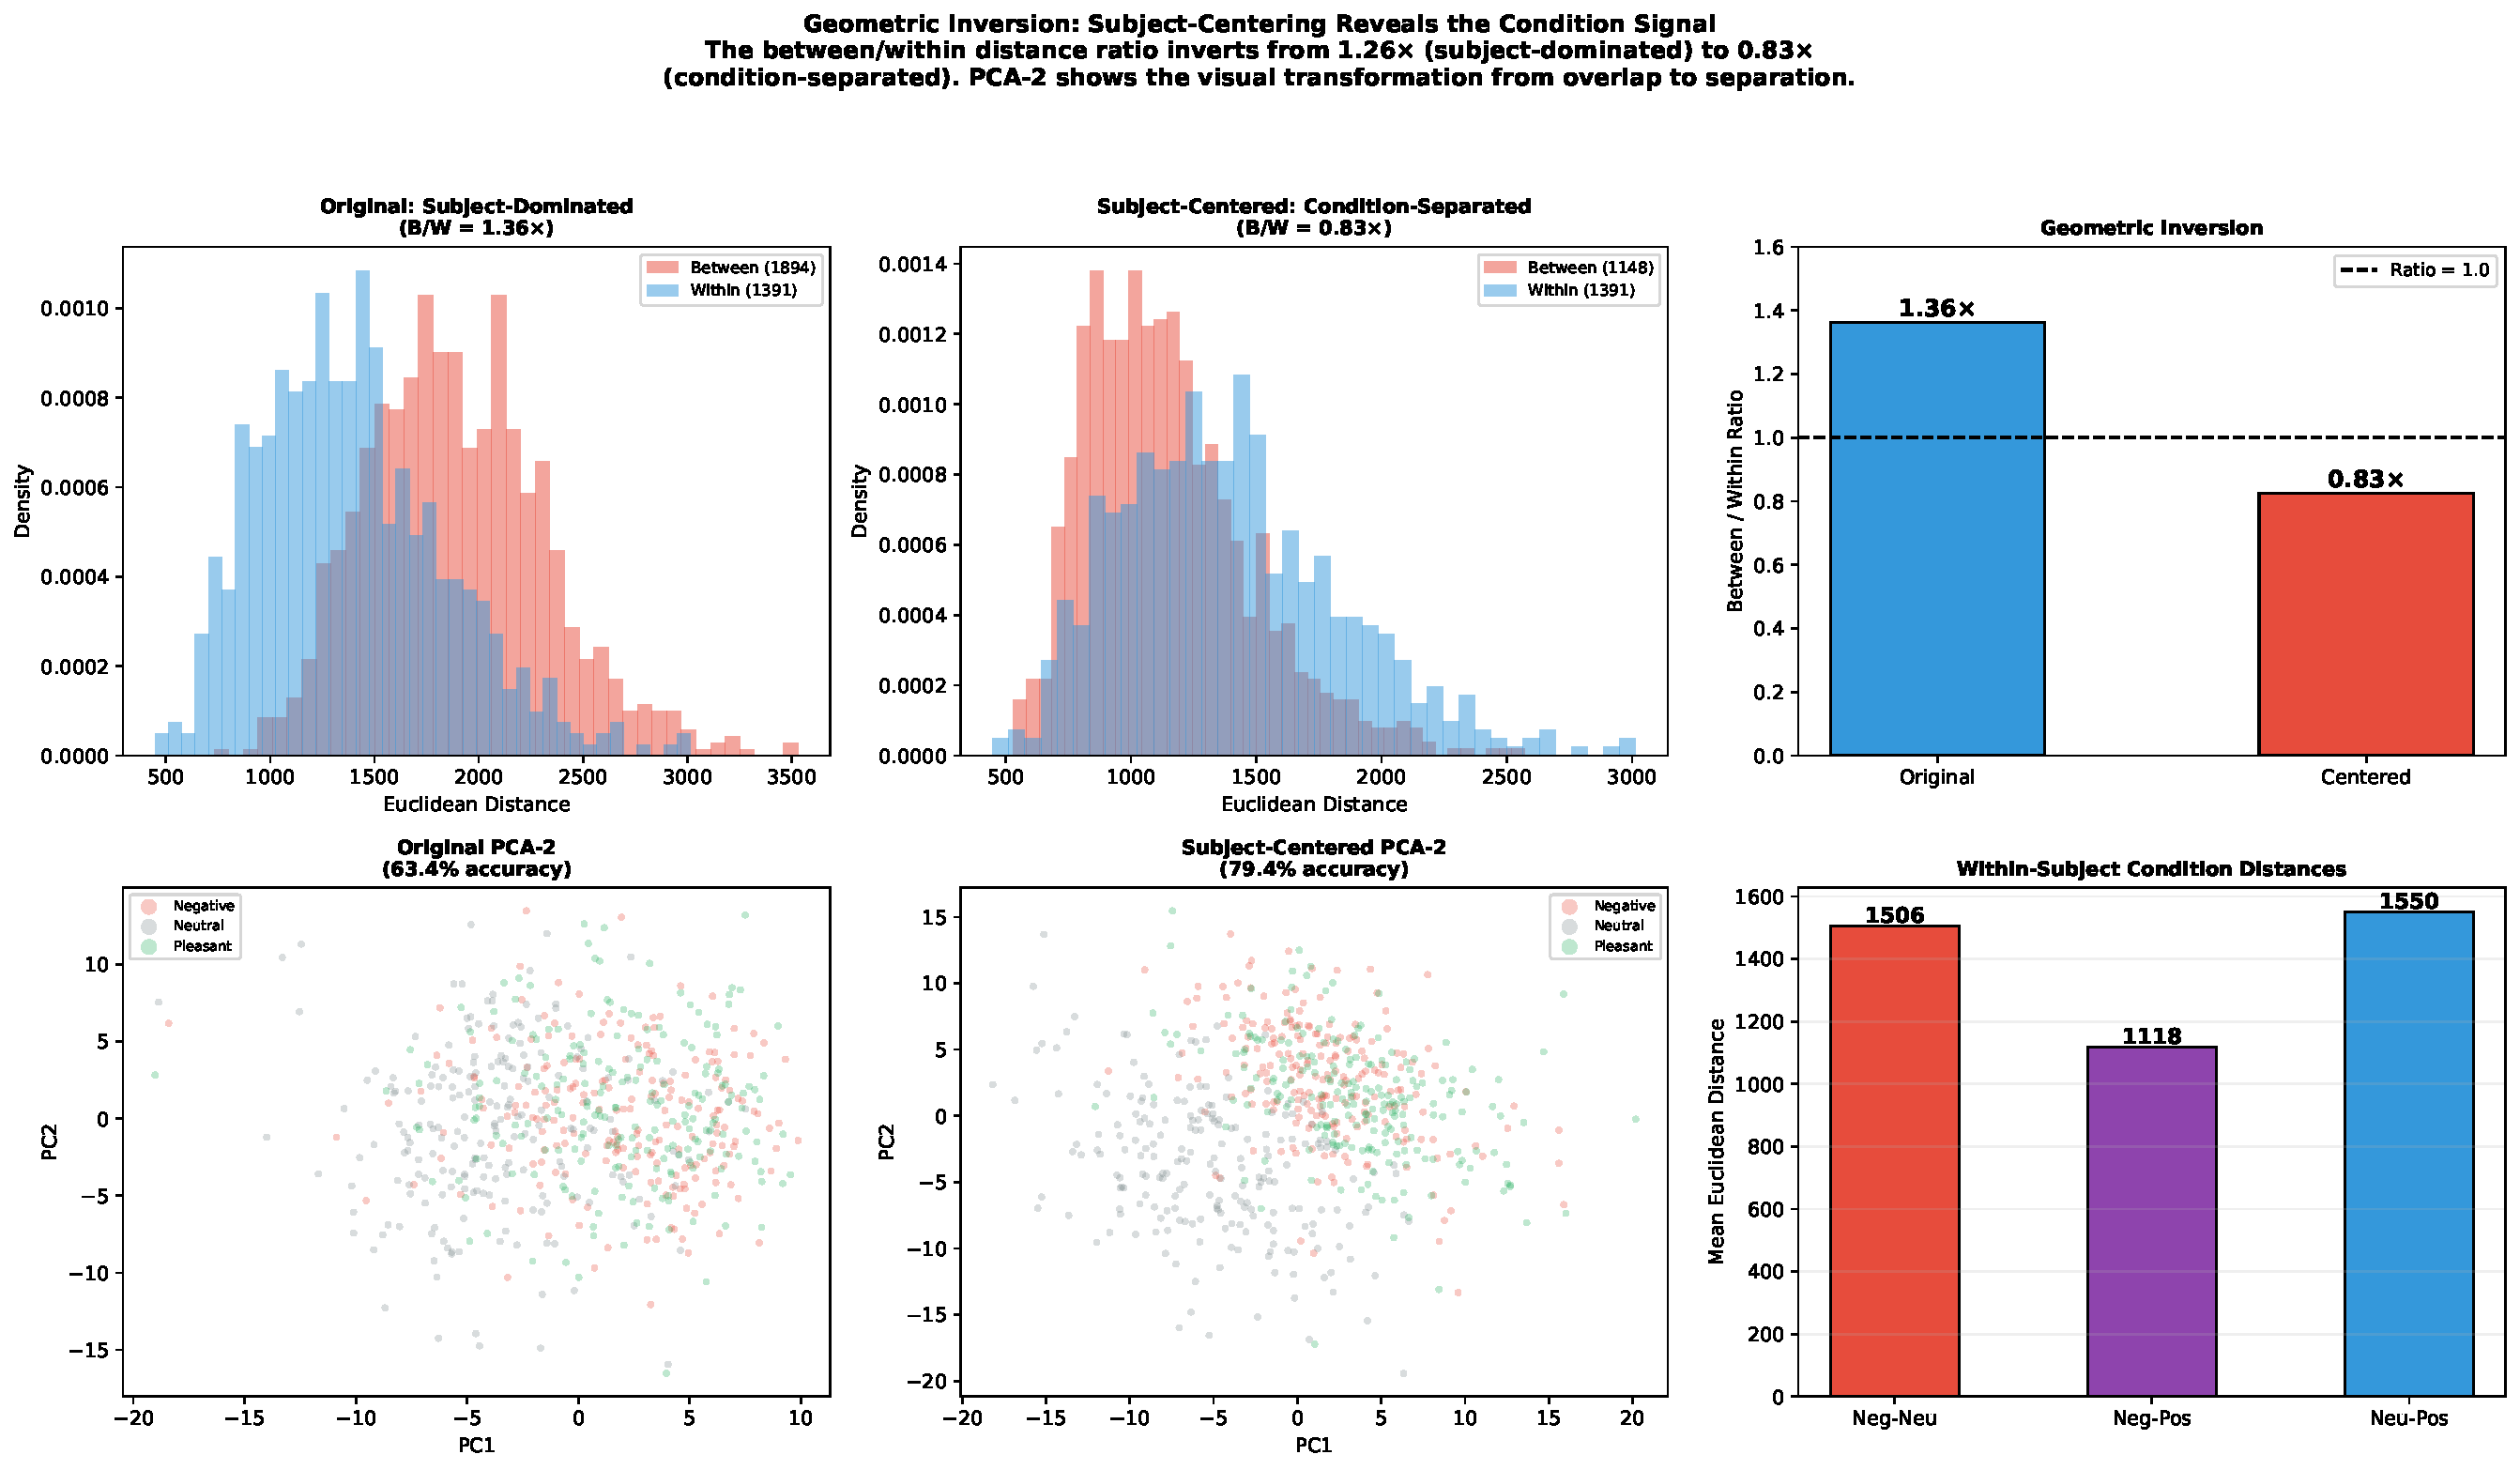
\includegraphics[width=\textwidth]{pictures/chGraphNeuralNetworks/obs14_within_between_geometry.pdf}
    \caption{Archived distance summaries before and after three-observation panel centering. The centered result is transductive, and the displayed PCA projections were fitted globally.}
    \label{fig:obs14_geometry}
\end{figure}

In the original embedding, the mean between-subject distance is $1{,}894$ and the mean within-subject cross-condition distance is $1{,}506$ (ratio $1.26$). After panel centering, the corresponding values are $1{,}148$ and $1{,}391$ (ratio $0.83$). This change is partly induced by the centering operation itself. Negative--Pleasant has the smallest displayed within-subject distance, but arousal was not modeled and is not inferred from that ordering.

The comparison shows how the chosen panel-centering operation changes the sample geometry. It does not isolate a biological nuisance component or reveal a ``true'' classification capacity. The associated $79.4\%$ value is a transductive, global-PCA legacy estimate.

\subsection{Graph Edge Stability Under Bootstrap Resampling}

Figure~\ref{fig:obs15_stability} records edge-selection frequencies across $200$ bootstrap resamples of the same subject pool. Of $561$ possible edges, $109$ are selected in more than $90\%$ of resamples, while $449$ are selected in fewer than $50\%$. These are internal selection frequencies under the same archived preprocessing, not test--retest reliability or independent-sample reproducibility.

The center panel shows that selection frequency varies by channel pair. Because the PCA-axis problem persists in every resample, frequent selection does not make an edge physiologically interpretable.

\begin{figure}[H]
    \centering
    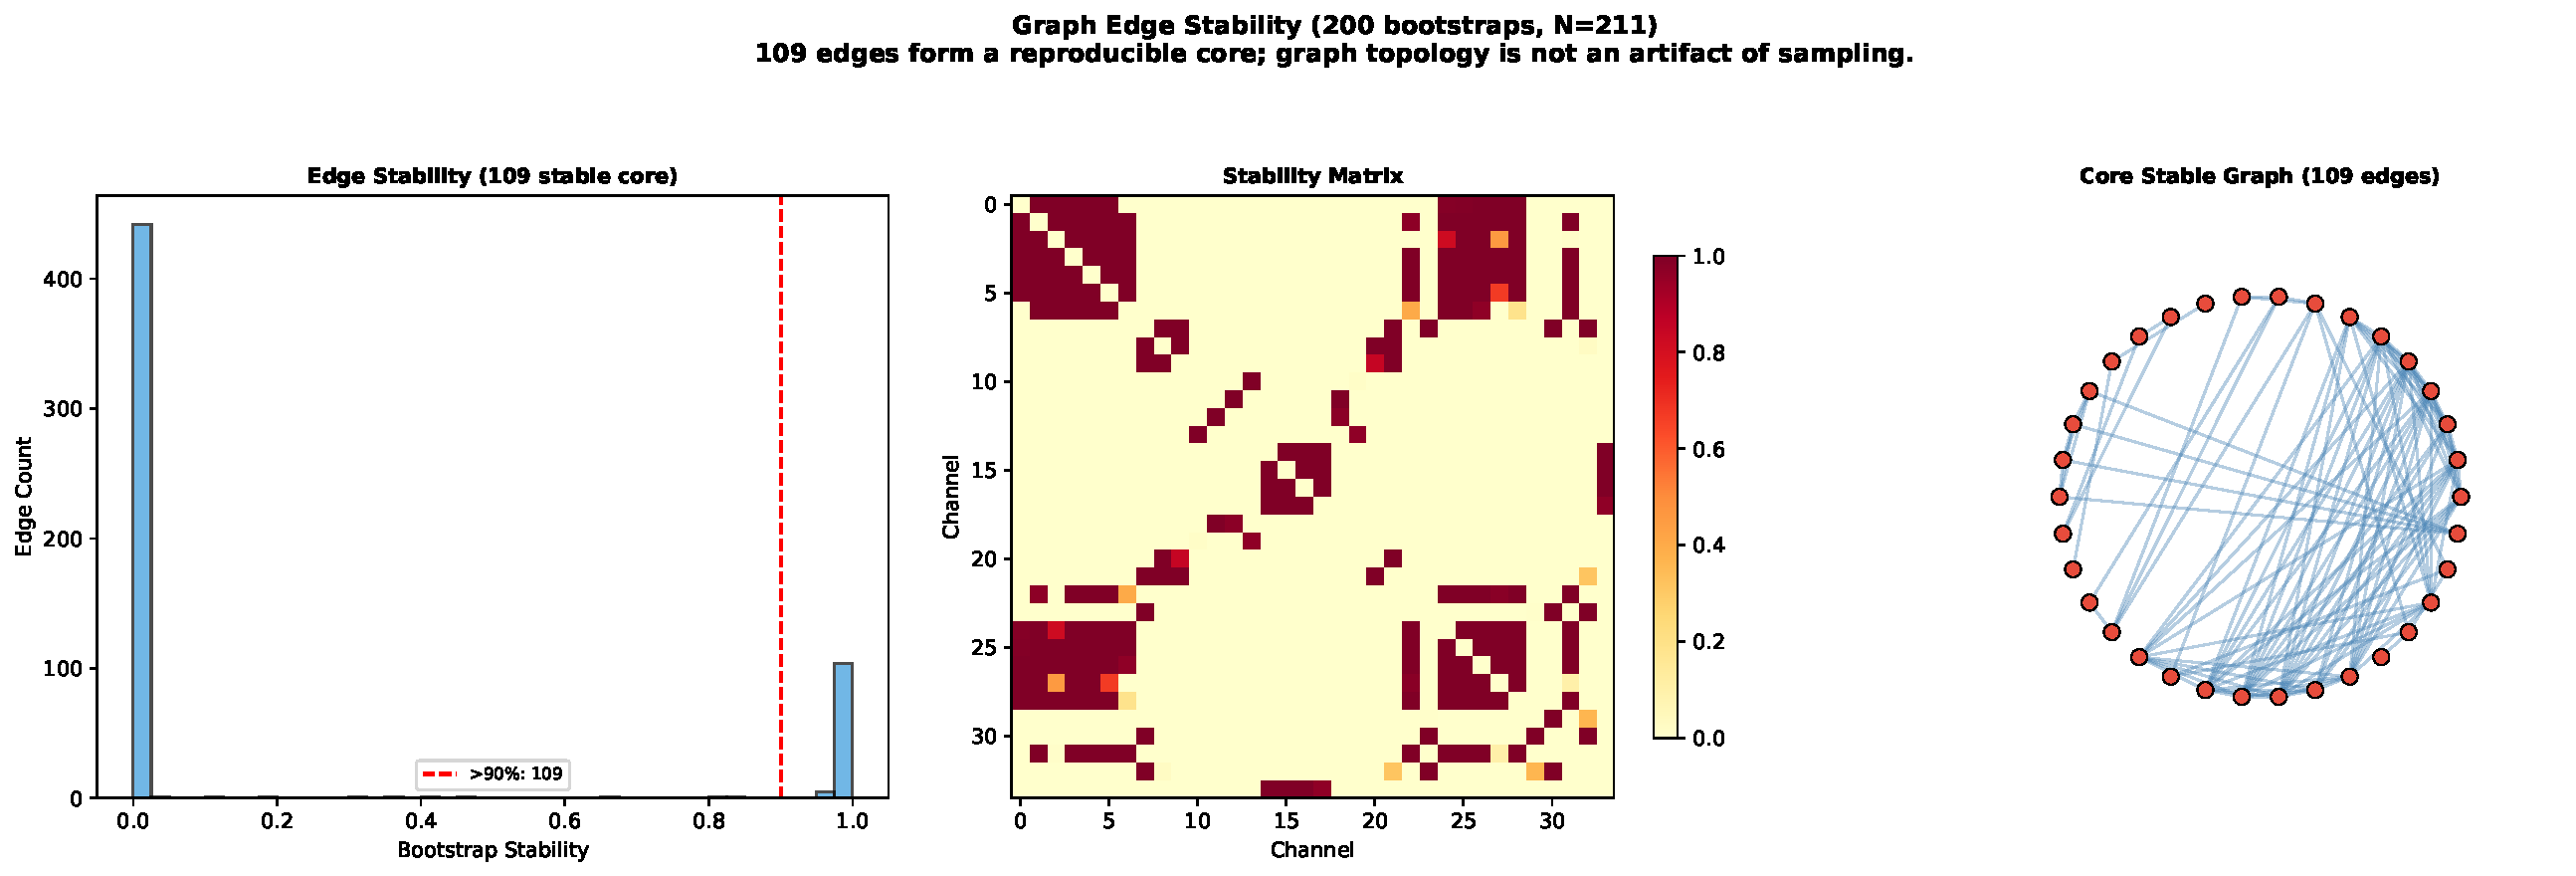
\includegraphics[width=\textwidth]{pictures/chGraphNeuralNetworks/obs15_edge_stability.pdf}
    \caption{Internal edge-selection frequencies across $200$ bootstrap resamples. Frequencies quantify stability under resampling of this cohort, not independent replication or physiological reliability.}
    \label{fig:obs15_stability}
\end{figure}

\subsection{Feature-Scale Changes Through the Pipeline}

Figure~\ref{fig:obs16_amplification} displays absolute Negative--Neutral differences after several transformations. The bars use different units and dimensional aggregations: z-scored amplitude, spike counts, sums of PCA coordinates, and centered PCA coordinates. Their heights are not comparable measures of a common signal and cannot demonstrate amplification.

The figure is retained to show the scale of each archived representation. A valid amplification comparison would require a common standardized effect or fold-wise predictive measure at every stage.

\begin{figure}[H]
    \centering
    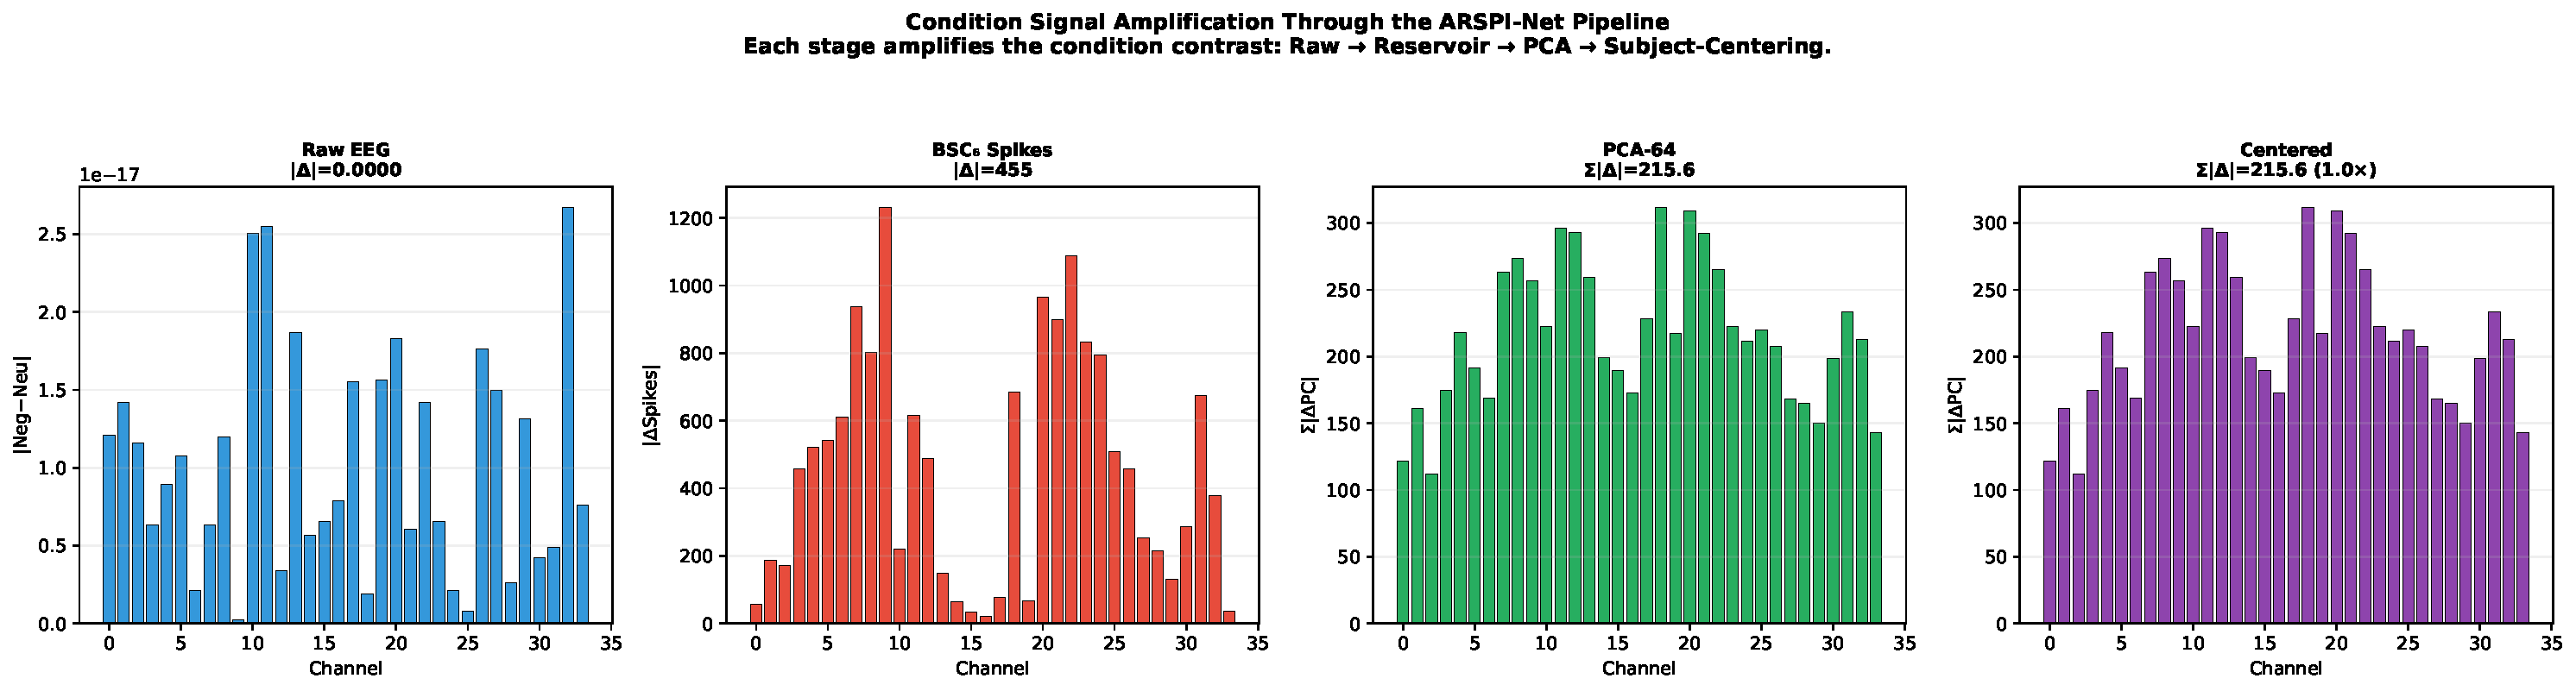
\includegraphics[width=\textwidth]{pictures/chGraphNeuralNetworks/obs16_signal_amplification.pdf}
    \caption{Archived absolute condition differences at successive pipeline stages. Bar heights use incompatible units and aggregations and therefore must not be compared as amplification factors.}
    \label{fig:obs16_amplification}
\end{figure}

\subsection{Graph Laplacian Spectral Characterization}

The Laplacian $\mathbf{L}=\mathbf{D}-\mathbf{A}$ summarizes the archived thresholded graph, and its eigenspectrum determines the action of linear polynomial filters on that graph. Figure~\ref{fig:obs17_spectral} records these mathematical properties; it does not establish properties of an anatomical electrode network.

\begin{figure}[H]
    \centering
    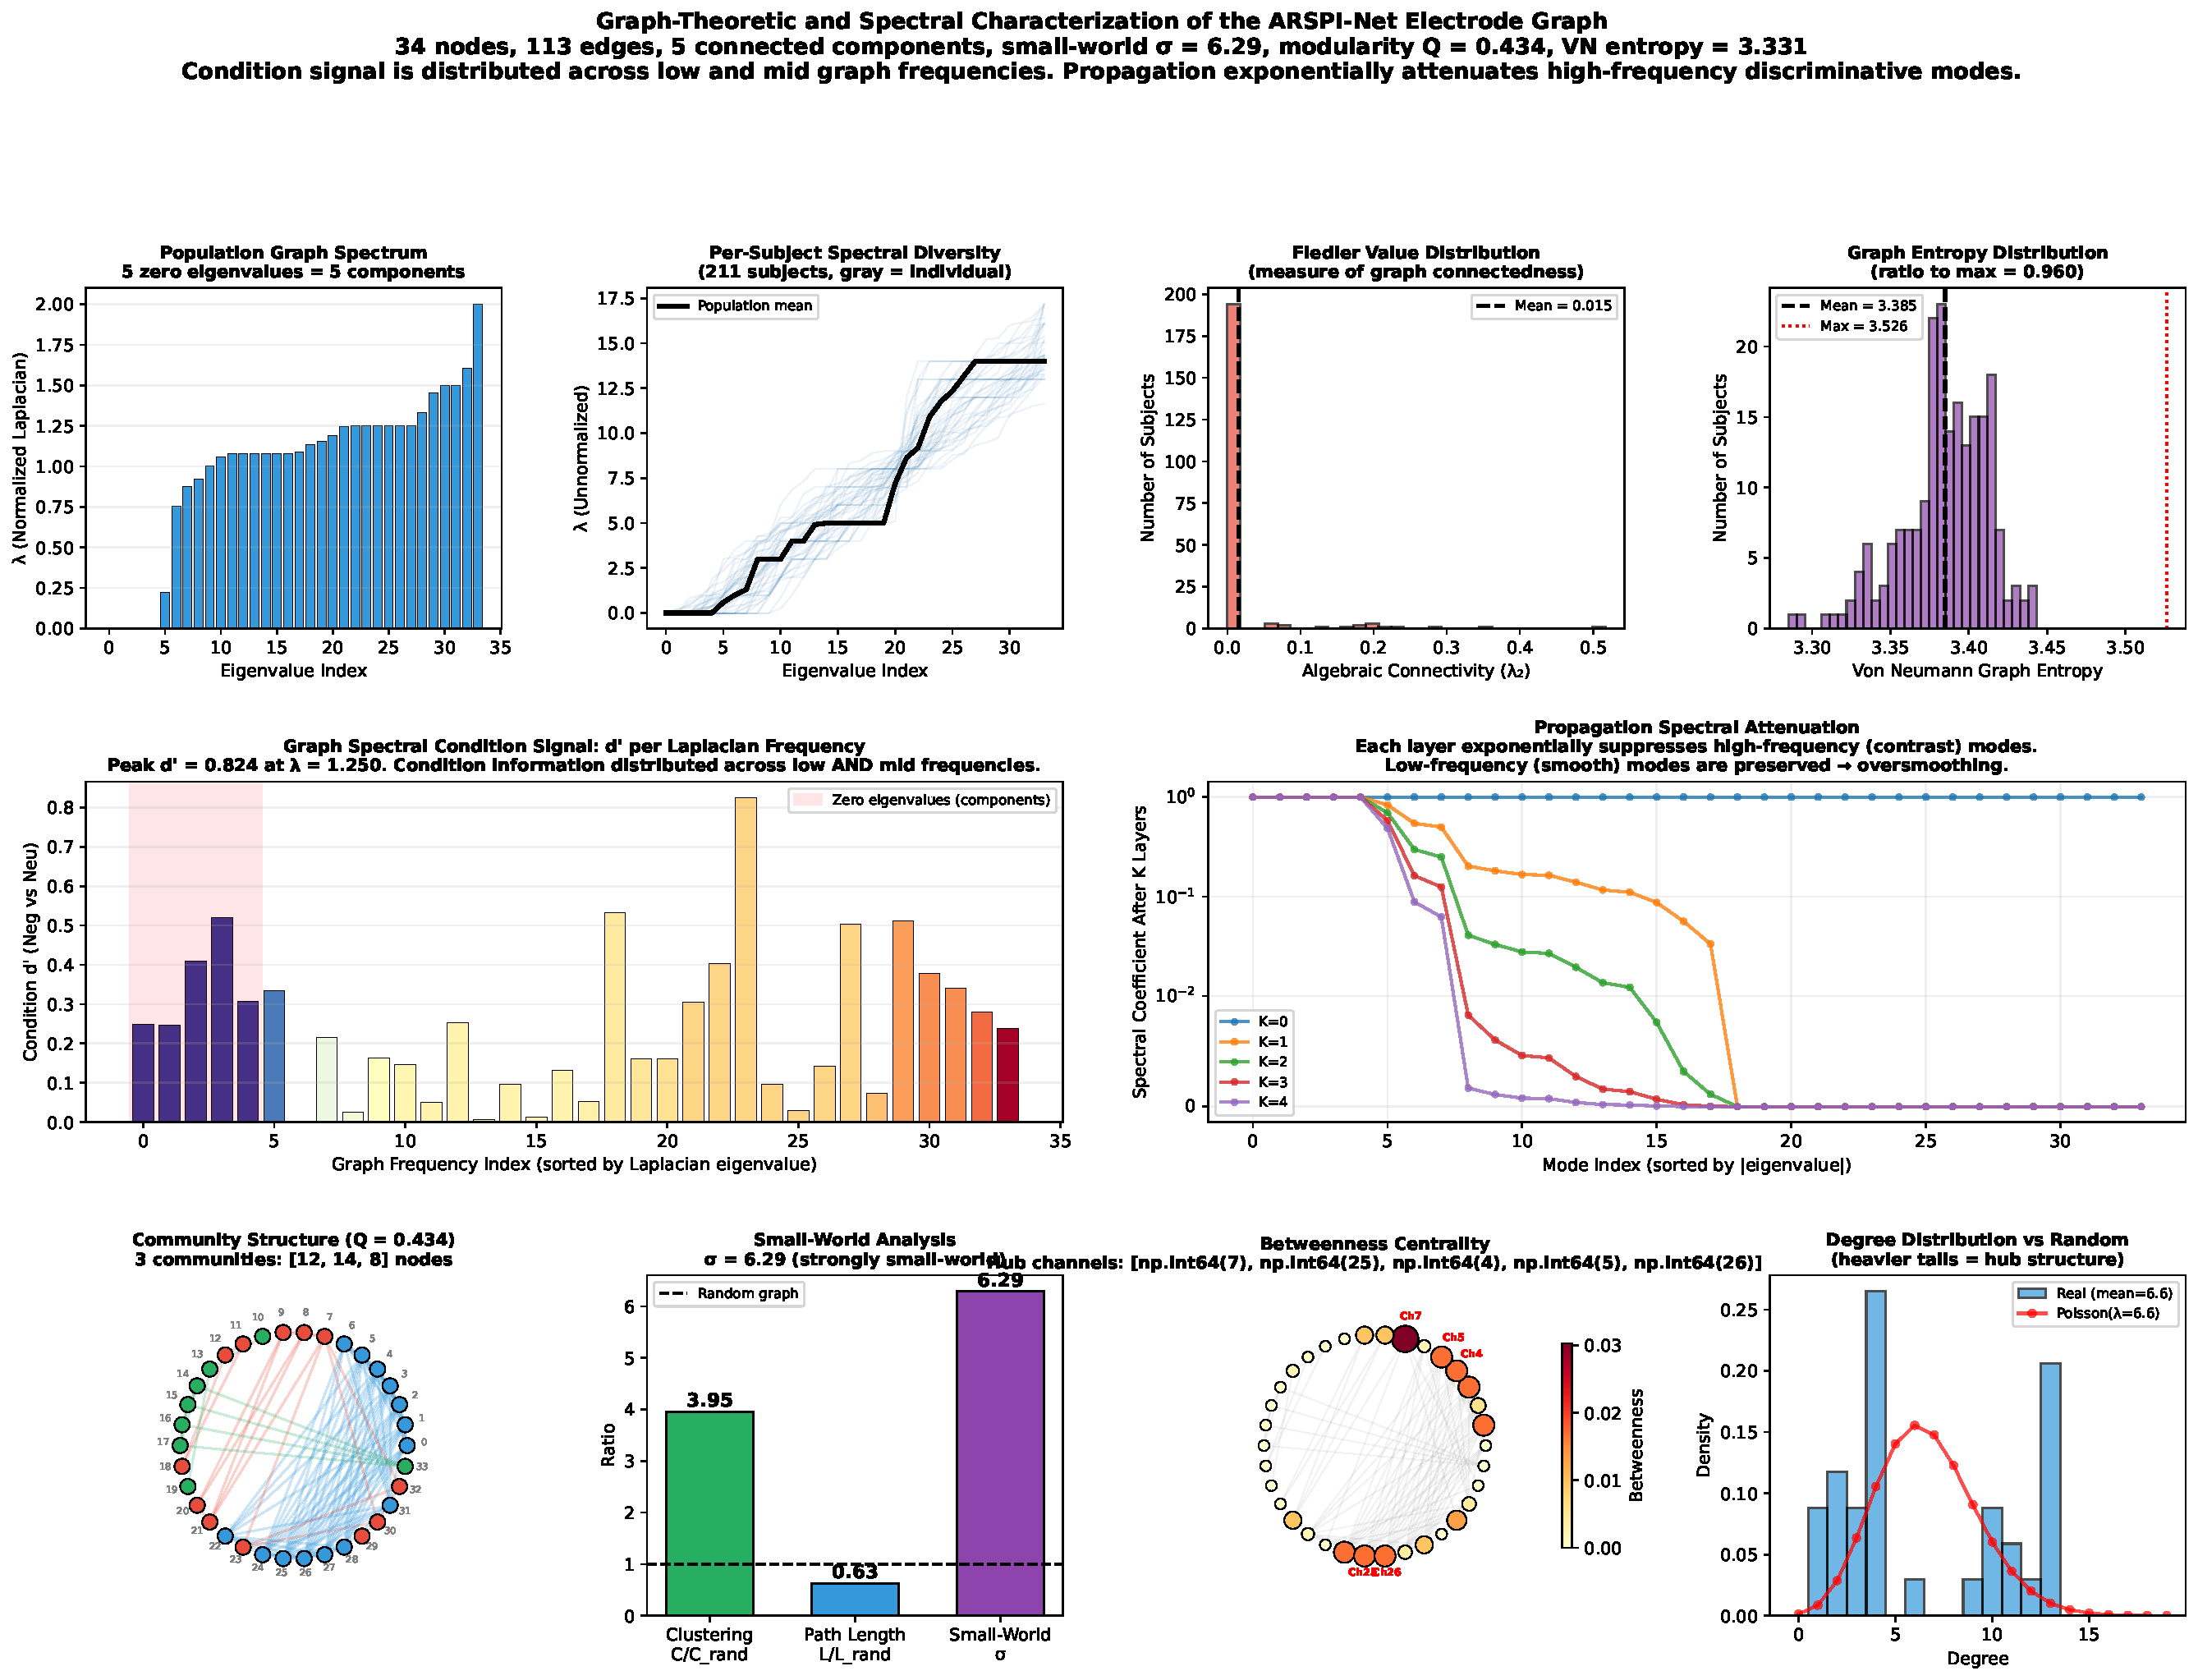
\includegraphics[width=\textwidth]{pictures/chGraphNeuralNetworks/obs17_spectral_analysis.pdf}
    \caption{Spectral summaries of the archived thresholded similarity graph. Values inherit the noncommensurate-PCA-basis limitation and have no anatomical interpretation.}
    \label{fig:obs17_spectral}
\end{figure}

The normalized Laplacian of the population-average graph has five zero eigenvalues, corresponding to five connected components at the $20\%$ threshold. Its Fiedler value is therefore effectively zero. Across participant-specific graphs, the displayed Fiedler value is $0.015 \pm 0.061$. The von Neumann graph-entropy calculation gives $3.331$, or $0.945$ of $\ln 34=3.526$; the participant-specific mean is $3.385\pm0.028$. These are properties of the legacy thresholded matrices, not evidence about robustness to perturbations or neural-network complexity.

The archived graph-Fourier panel displays Negative--Neutral d$'$ values across graph modes. Linear propagation attenuates modes according to their adjacency eigenvalues, but the panel does not show that attenuated modes uniquely carry condition information or that standardized detectability must fall.

After $K$ layers of normalized linear propagation, the $i$th mode is multiplied by $\mu_i^K$. Modes with $|\mu_i|<0.2$ retain less than $4\%$ of their squared amplitude after two layers. This algebraic attenuation is reversible only if the operator is invertible and numerically stable; it should not be equated with a measured loss of mutual information.

\subsection{Archived Small-World and Community Summaries}

The archived thresholded graph has a high clustering-to-random ratio and short paths within its largest component. Figure~\ref{fig:obs20_topology} summarizes these graph-theoretic values.

\begin{figure}[H]
    \centering
    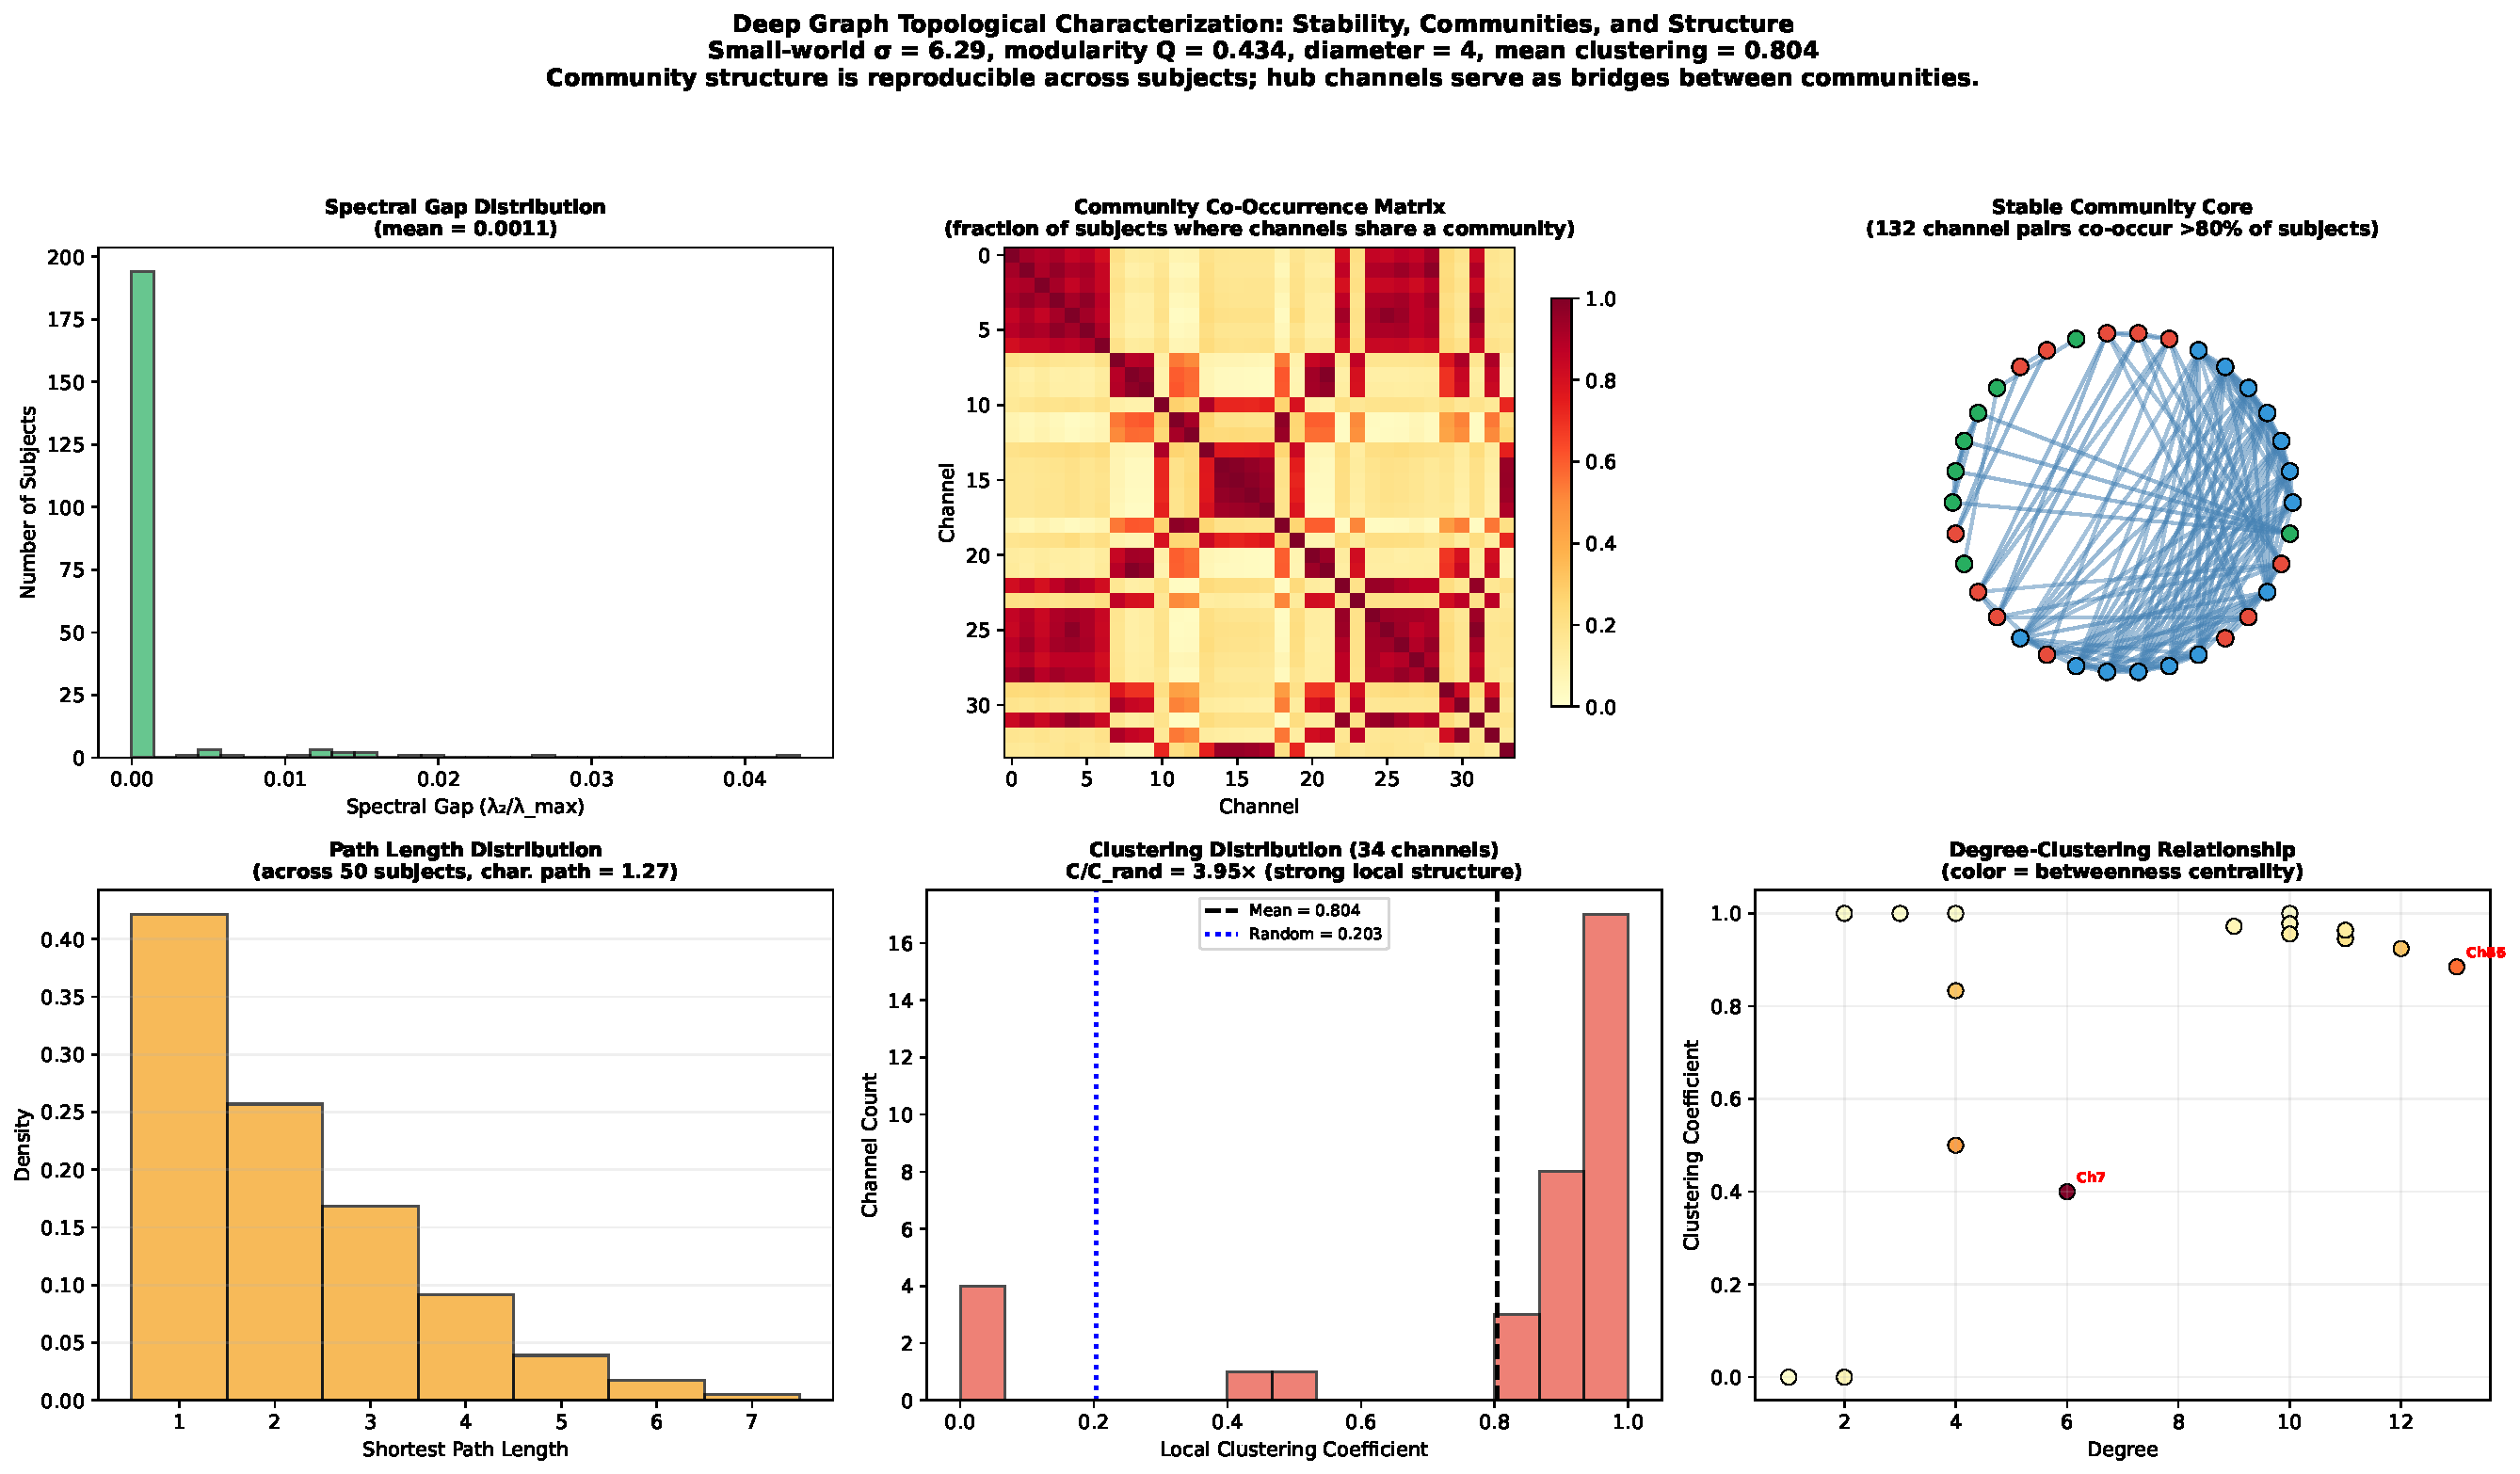
\includegraphics[width=\textwidth]{pictures/chGraphNeuralNetworks/obs20_deep_topology.pdf}
    \caption{Archived graph summaries. Top: spectral-gap distribution, community co-occurrence among channel indices, and pairs with more than $80\%$ co-occurrence. Bottom: largest-component path lengths, clustering relative to the selected degree-matched random-graph null, and degree--clustering values. Labels such as Ch7 and Ch25 are channel indices without anatomical assignments.}
    \label{fig:obs20_topology}
\end{figure}

The clustering coefficient is $3.95\times$ that of the selected degree-matched random graphs ($0.804$ versus $0.203$), and the reported largest-component path length is $1.27$ versus $2.01$, yielding $\sigma=6.29$. This value depends on the threshold, component convention, and random-graph null. It characterizes the legacy similarity graph and does not imply efficient neural communication \cite{rubinov_complex_2010}.

Hierarchical clustering produces three communities with modularity $Q=0.434$, and some channel-index pairs co-occur in more than $80\%$ of within-cohort resamples. These are algorithm-dependent groups of unlabeled indices. Terms such as ``community'' and ``bridge'' describe graph roles only and cannot be mapped to brain regions in the present data.

\subsection{Per-Subject Graph Topology Gallery}

Figure~\ref{fig:obs18_gallery} displays the archived graphs for $20$ randomly selected participants. Their component counts and clustering values vary. The exploratory clinical analyses below test selected group comparisons but do not establish that group effects rise above this variability.

\begin{figure}[H]
    \centering
    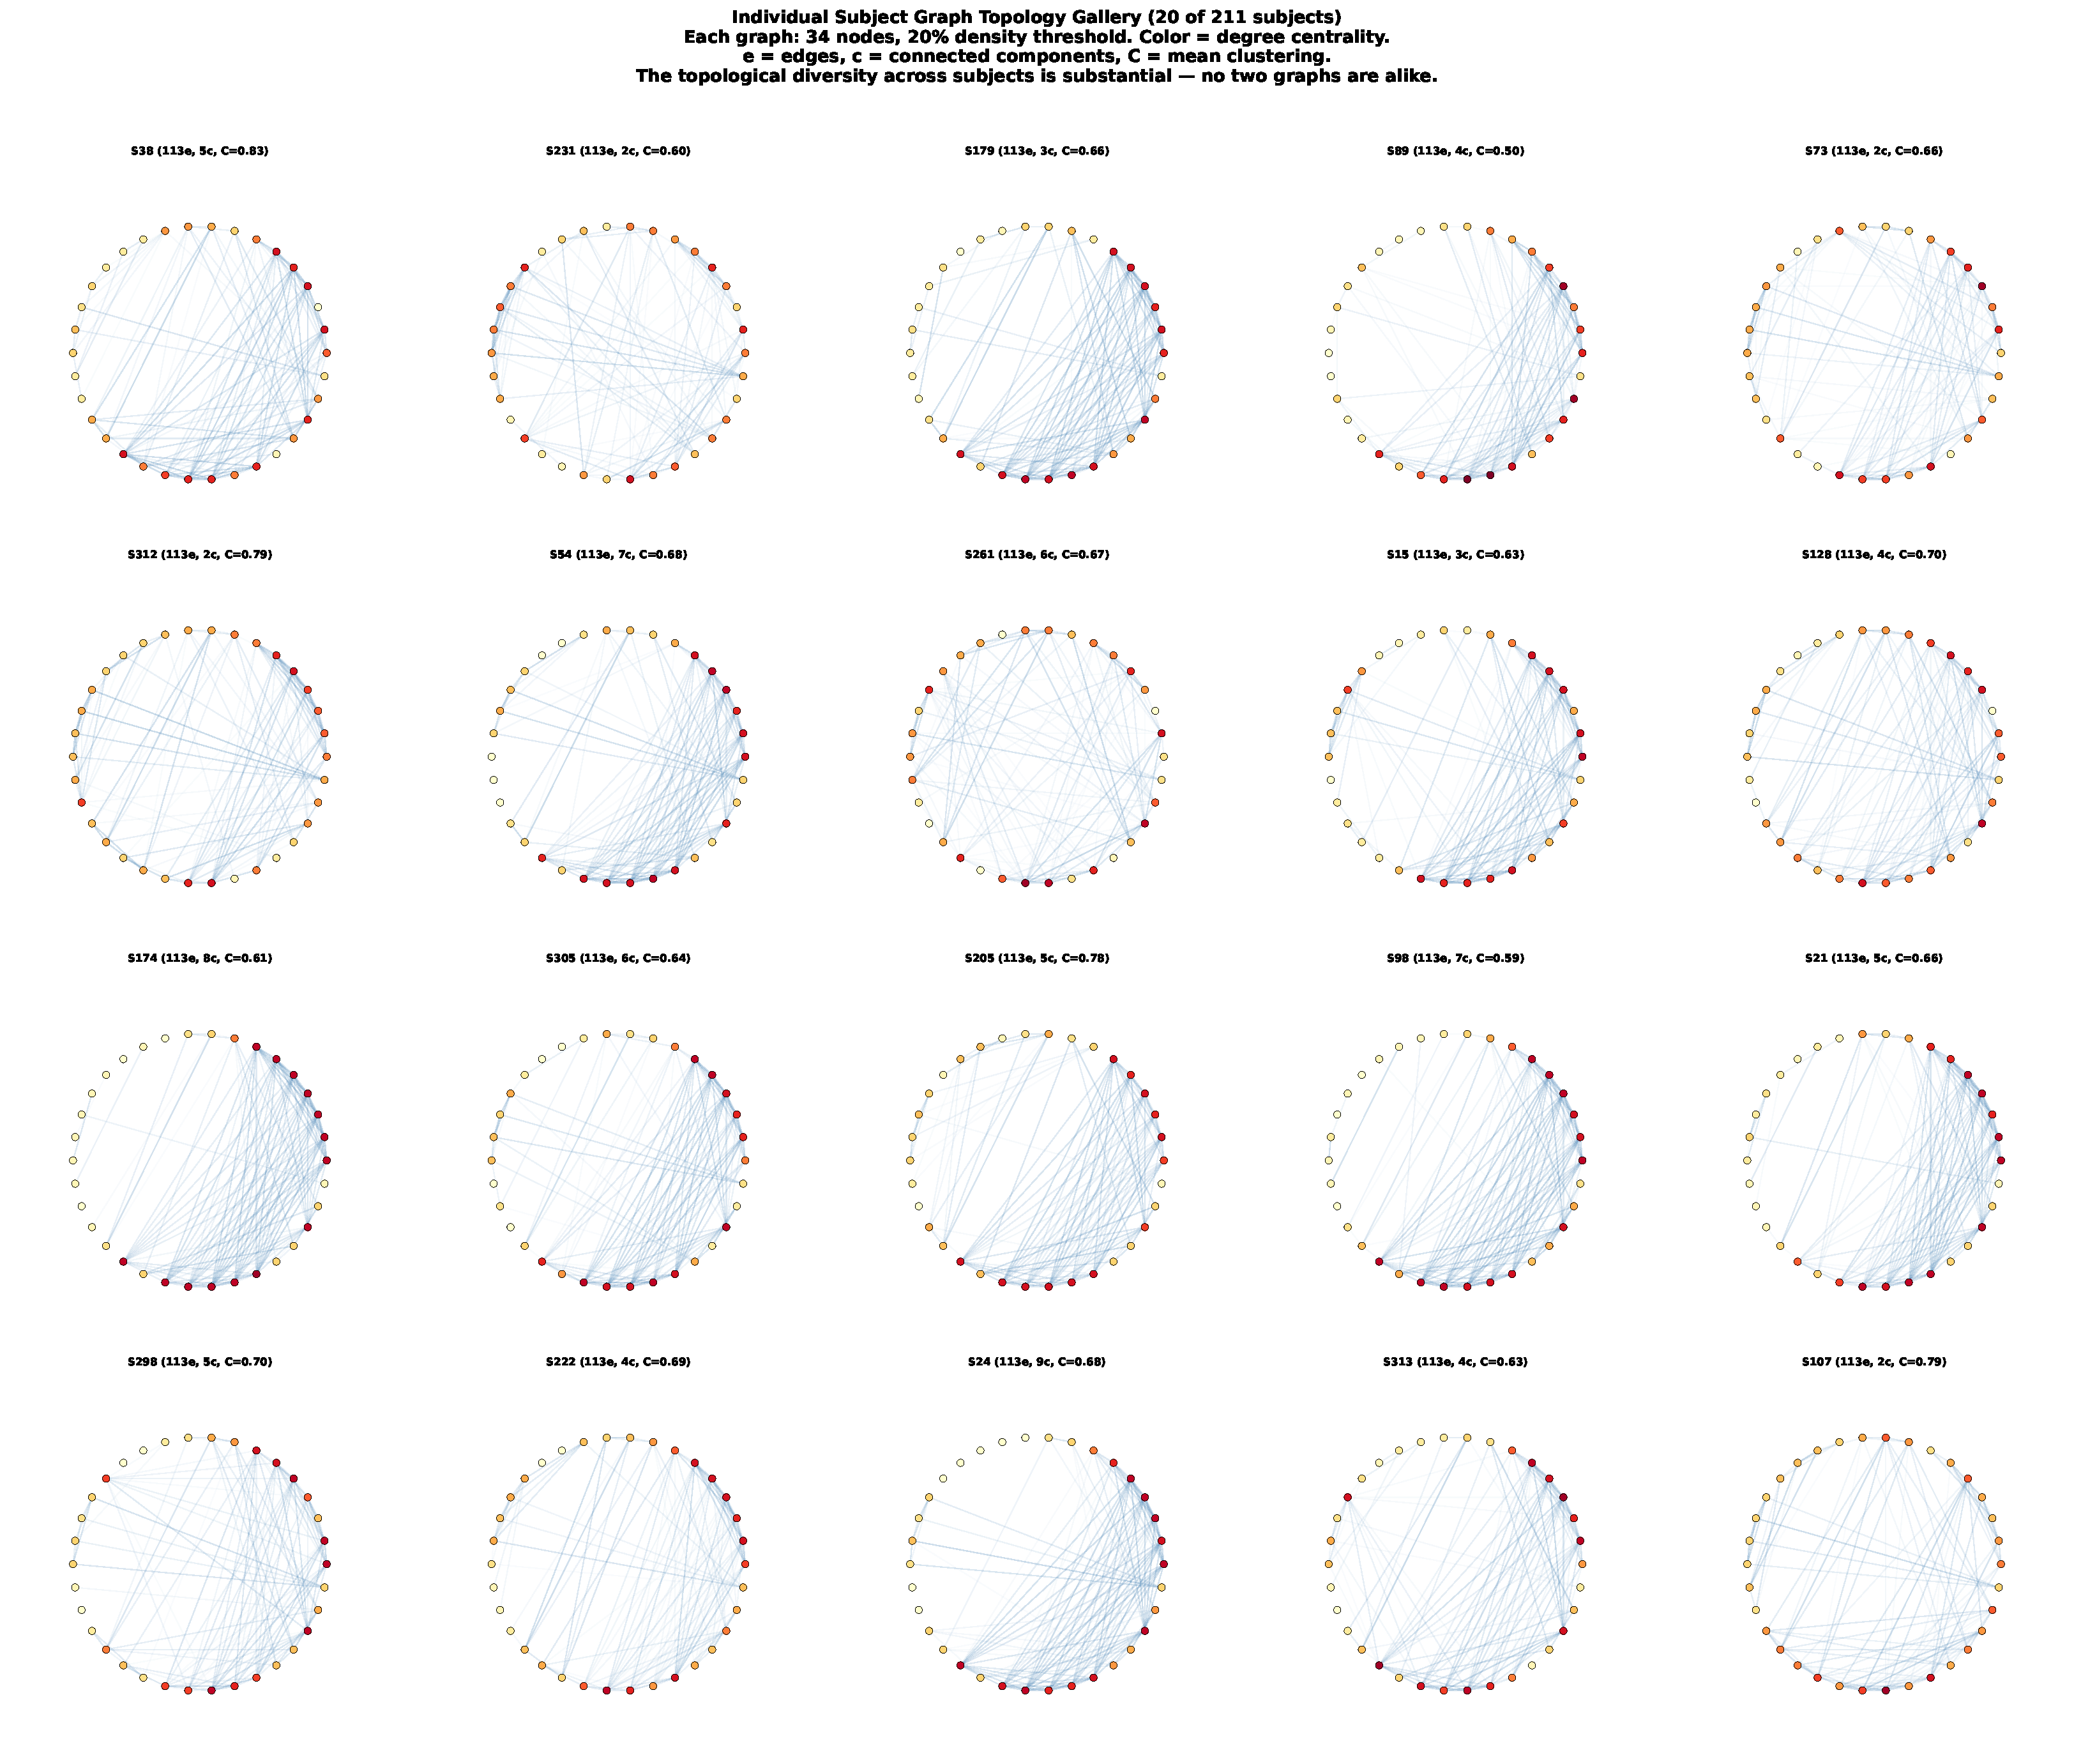
\includegraphics[width=\textwidth]{pictures/chGraphNeuralNetworks/obs18_subject_gallery.pdf}
    \caption{Archived graph gallery for $20$ of $211$ participants. Each graph has $34$ nodes and uses the $20\%$ density threshold. Node color shows degree centrality; $e$ denotes edges, $c$ connected components, and $\bar{C}$ mean clustering.}
    \label{fig:obs18_gallery}
\end{figure}

\subsection{Condition-Specific Graph Spectral Analysis}

Figure~\ref{fig:obs19_cond_spectral} compares the archived condition-specific graph spectra. The displayed eigenvalues and entropy summaries differ slightly by condition. No prespecified inferential test is reported for the full spectral family, and a higher graph entropy is not interpreted as greater physiological ``structural complexity.''

\begin{figure}[H]
    \centering
    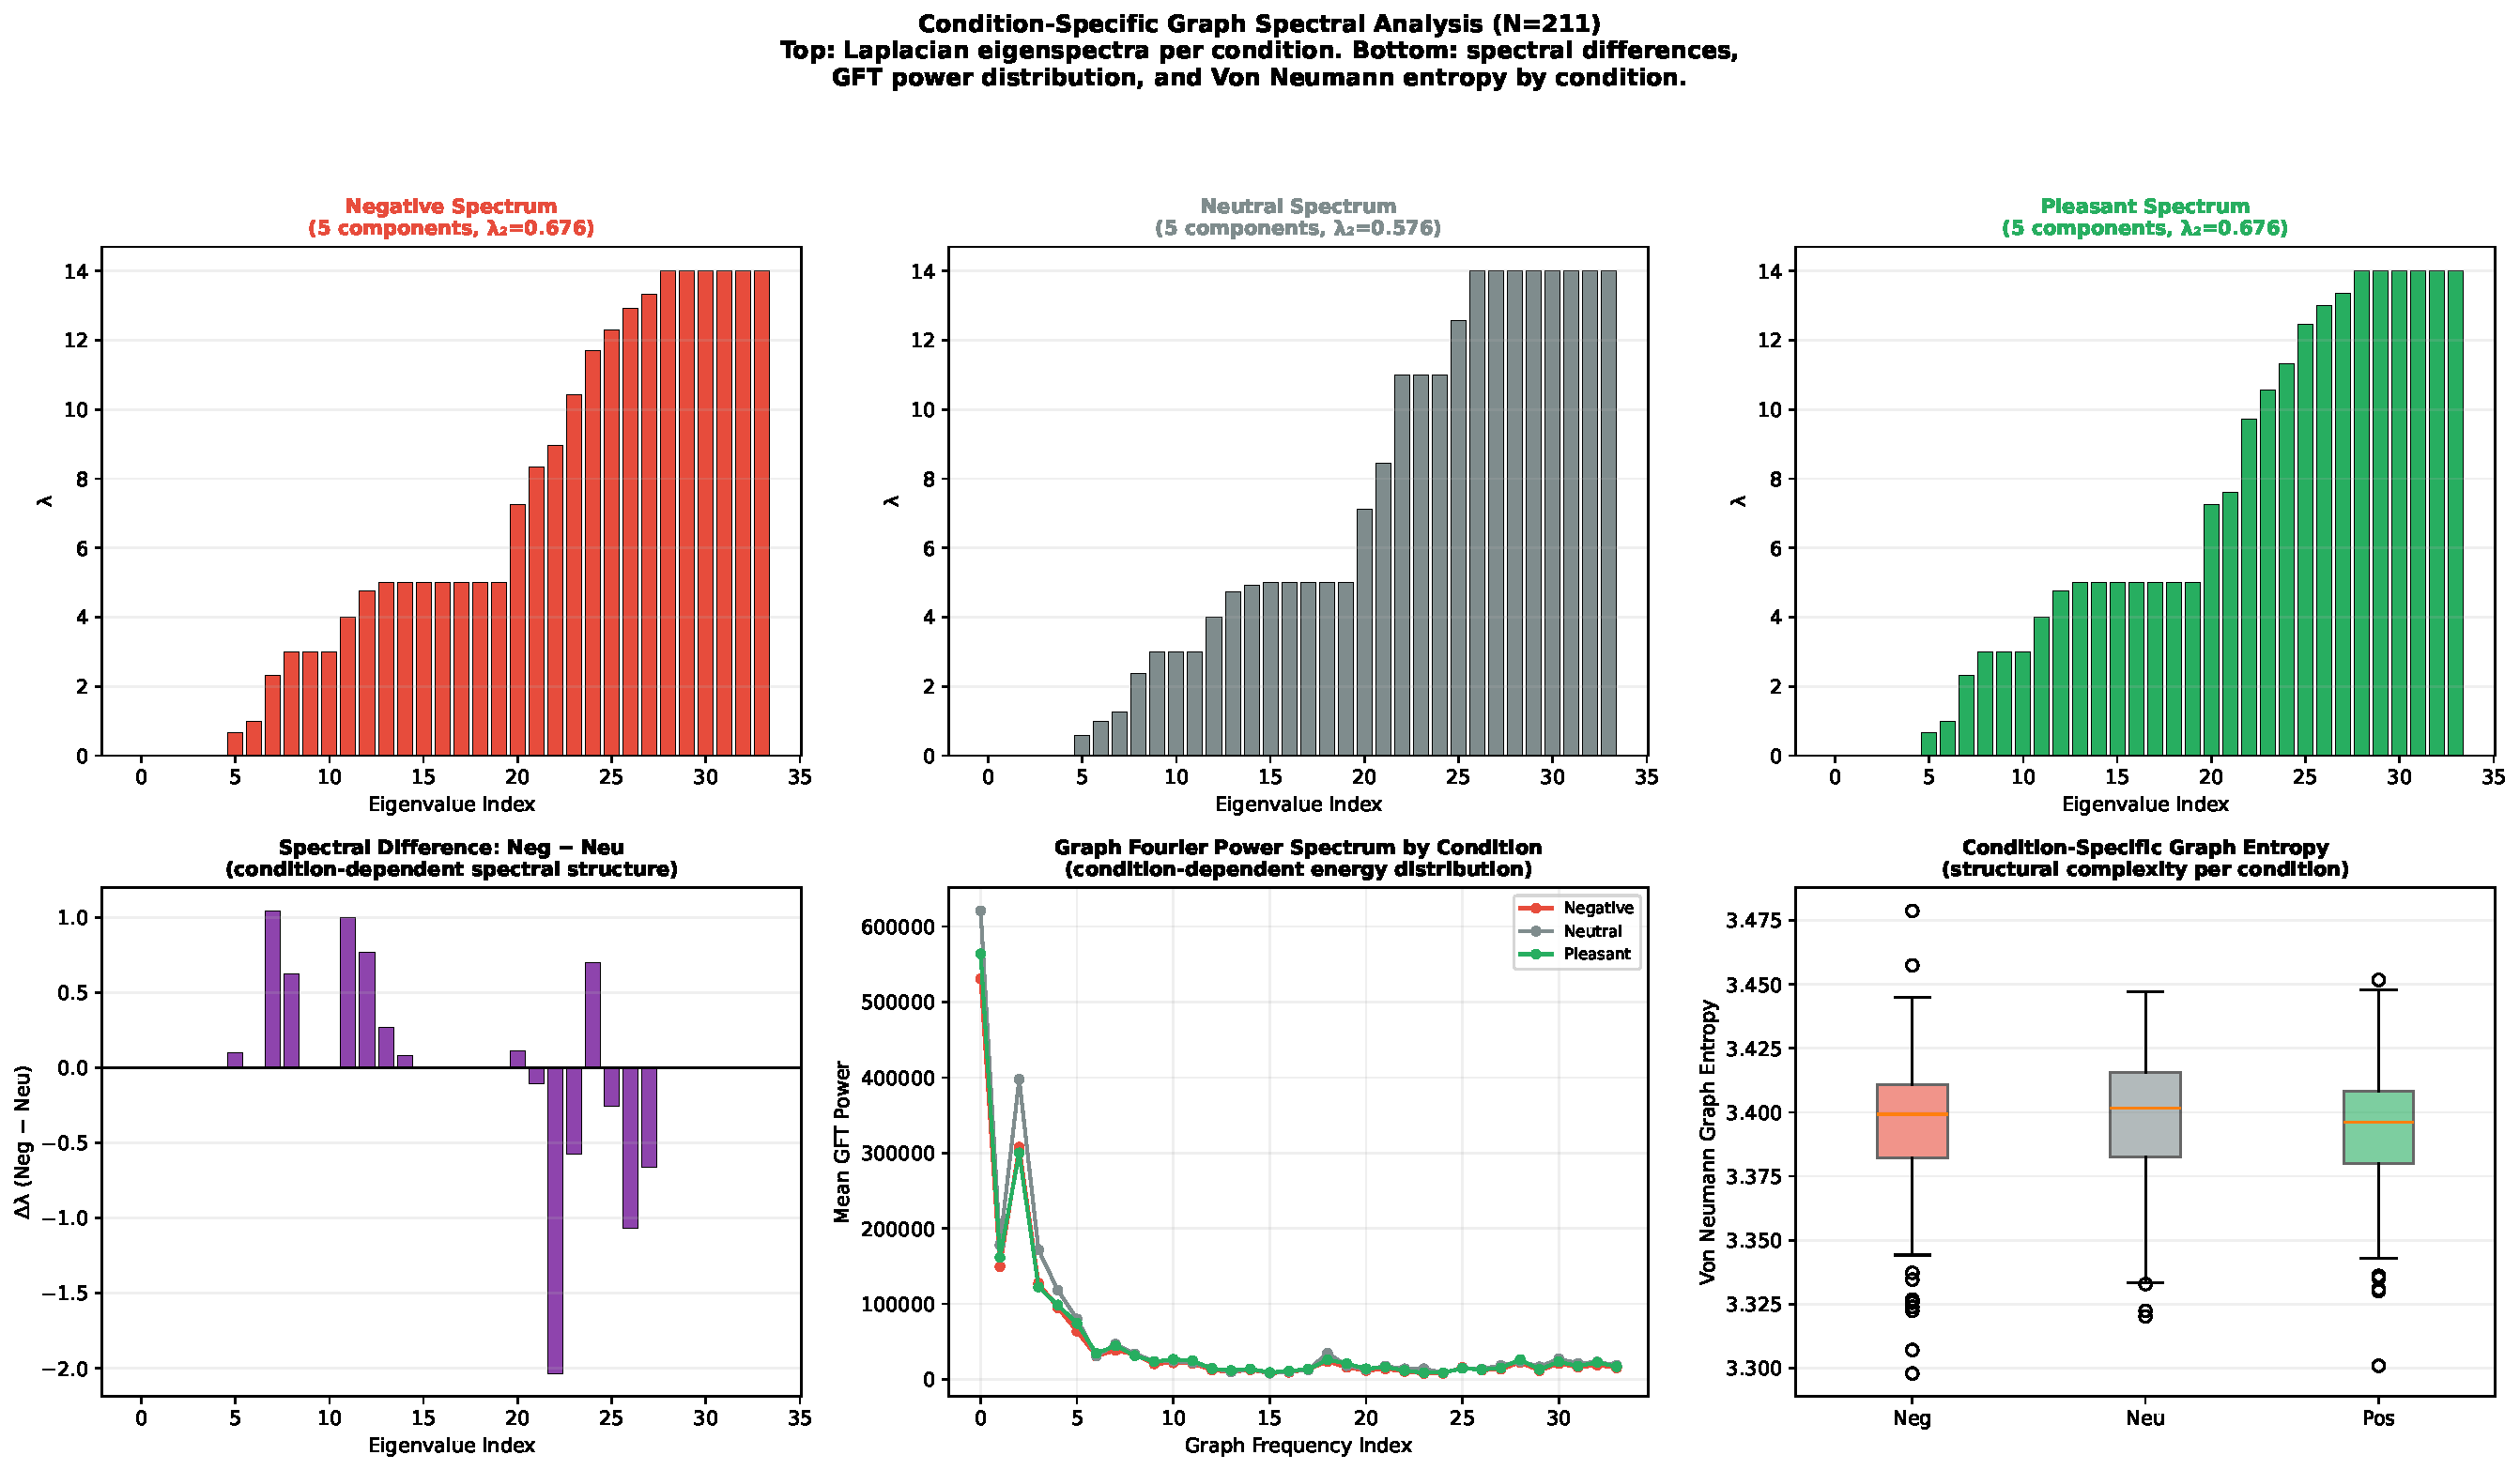
\includegraphics[width=\textwidth]{pictures/chGraphNeuralNetworks/obs19_condition_spectral.pdf}
    \caption{Archived condition-specific spectral summaries. Differences are descriptive and inherit the graph-construction limitations described in the text.}
    \label{fig:obs19_cond_spectral}
\end{figure}

\subsection{Grand-Average ERPs: The Condition Signal}

Figure~\ref{fig:obs08_erps} displays grand-average waveforms for four channel indices. Negative-minus-Neutral differences are small relative to the z-scored waveform range. Without verified electrode labels, component-specific channels, and prespecified windows, the figure is not used to claim an LPP effect.

\begin{figure}[H]
    \centering
    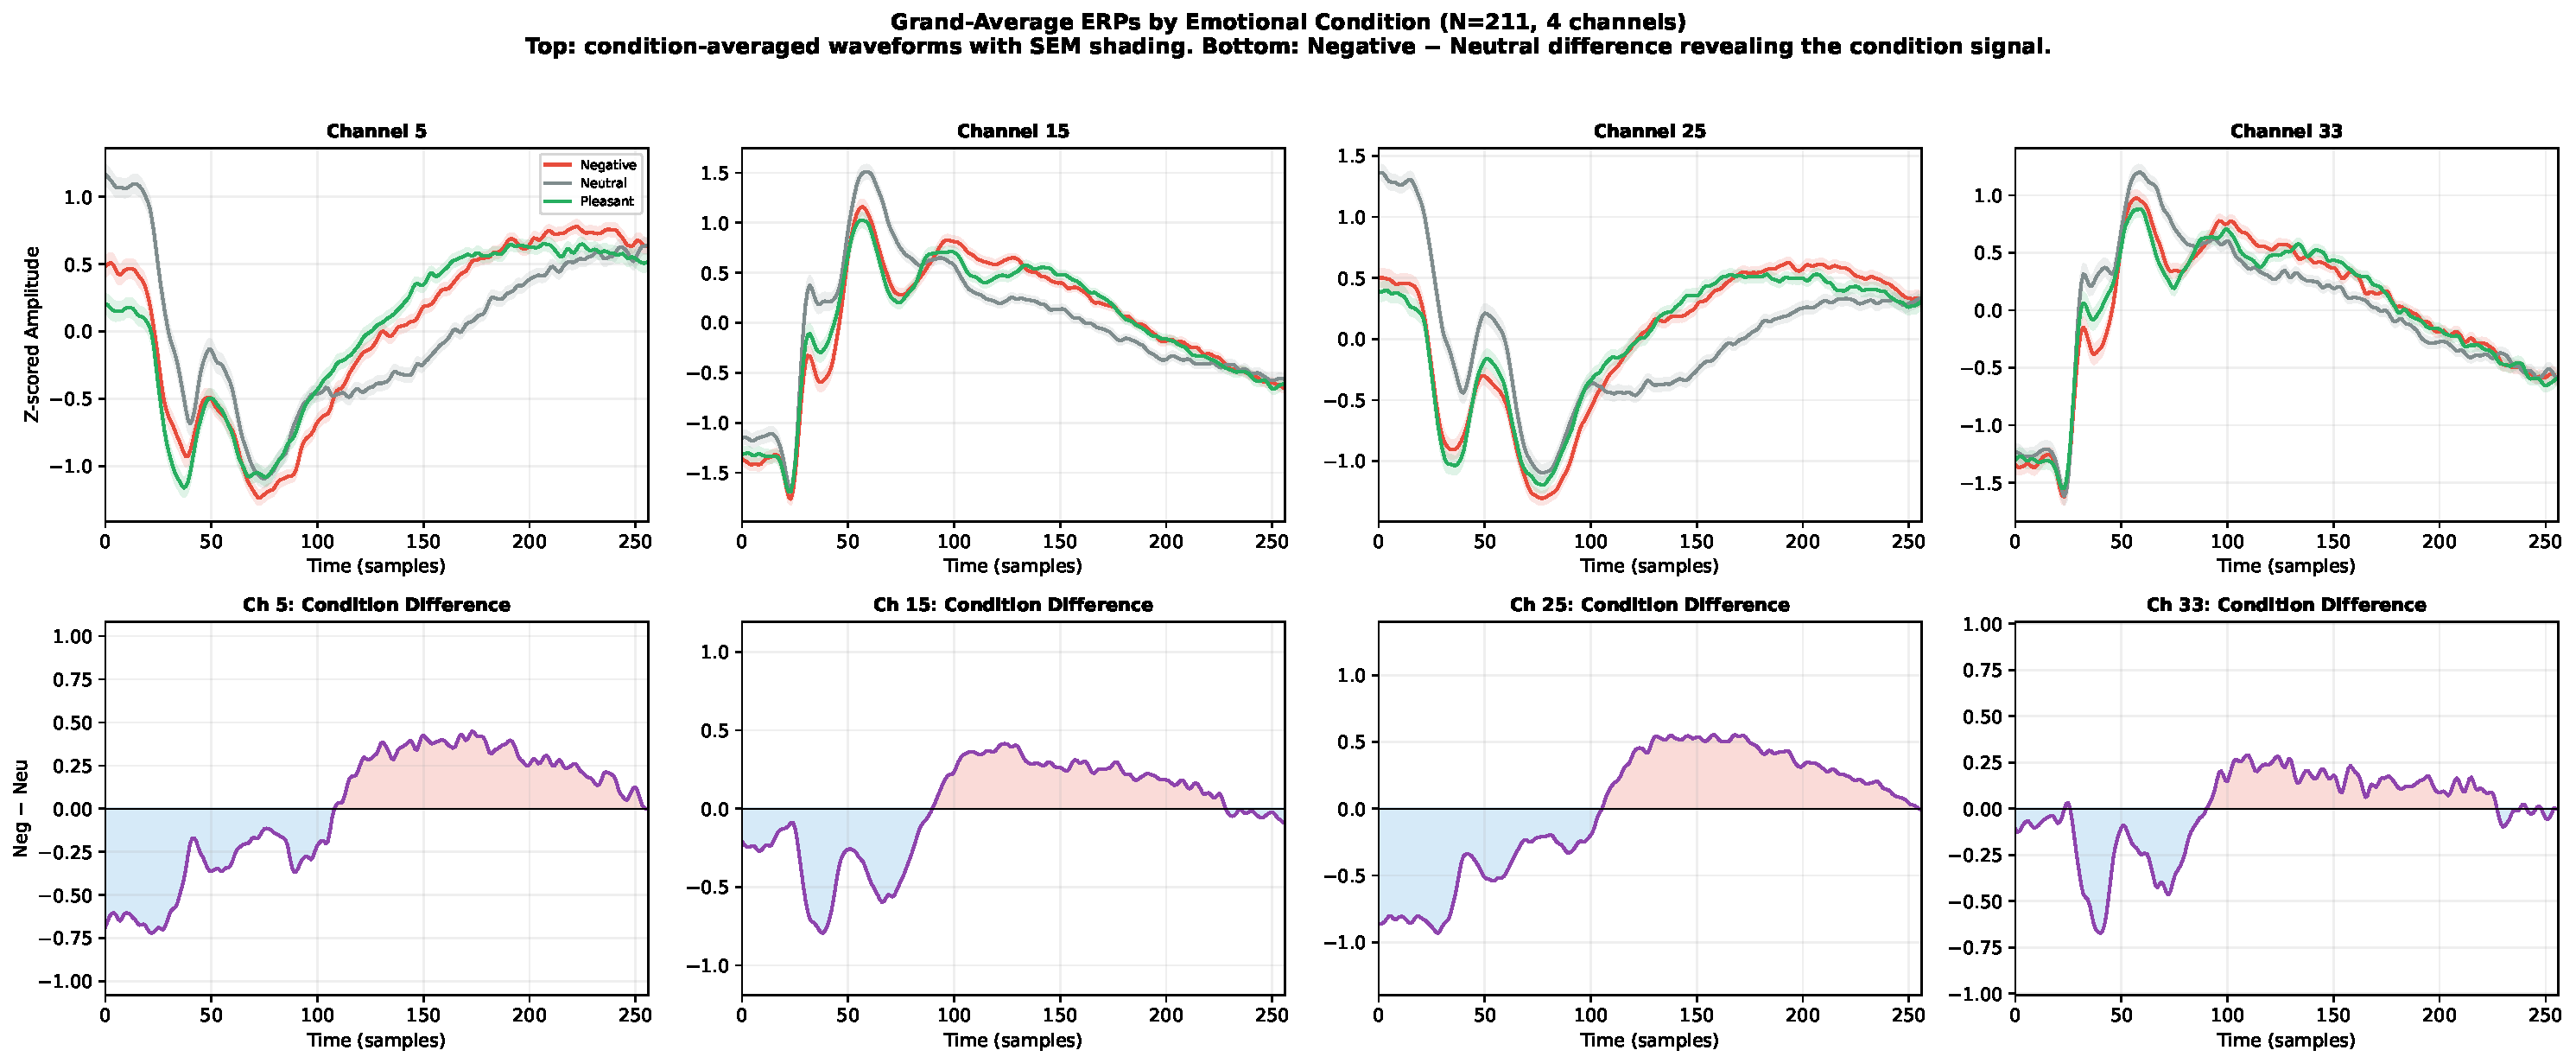
\includegraphics[width=\textwidth]{pictures/chGraphNeuralNetworks/obs08_grand_average_erps.pdf}
    \caption{Grand-average ERPs by condition ($N = 211$). Top: condition-averaged waveforms with SEM shading for four channels. Bottom: Negative $-$ Neutral difference waveforms. Condition effects are small ($5$--$15\%$ of z-scored amplitude) but temporally structured.}
    \label{fig:obs08_erps}
\end{figure}

\subsection{Synthetic-to-Real PCA Transfer Verification}

In the globally fitted per-channel PCA models, $64$ components explain $99.3\%$ of sample variance and the mean component count at $90\%$ variance is seven. Explained variance is not equivalent to retaining class information. Similar eigenvalue spectra also do not make separately fitted component axes comparable across channels. A fold-local common-basis analysis is required for downstream graph construction.

\begin{figure}[H]
    \centering
    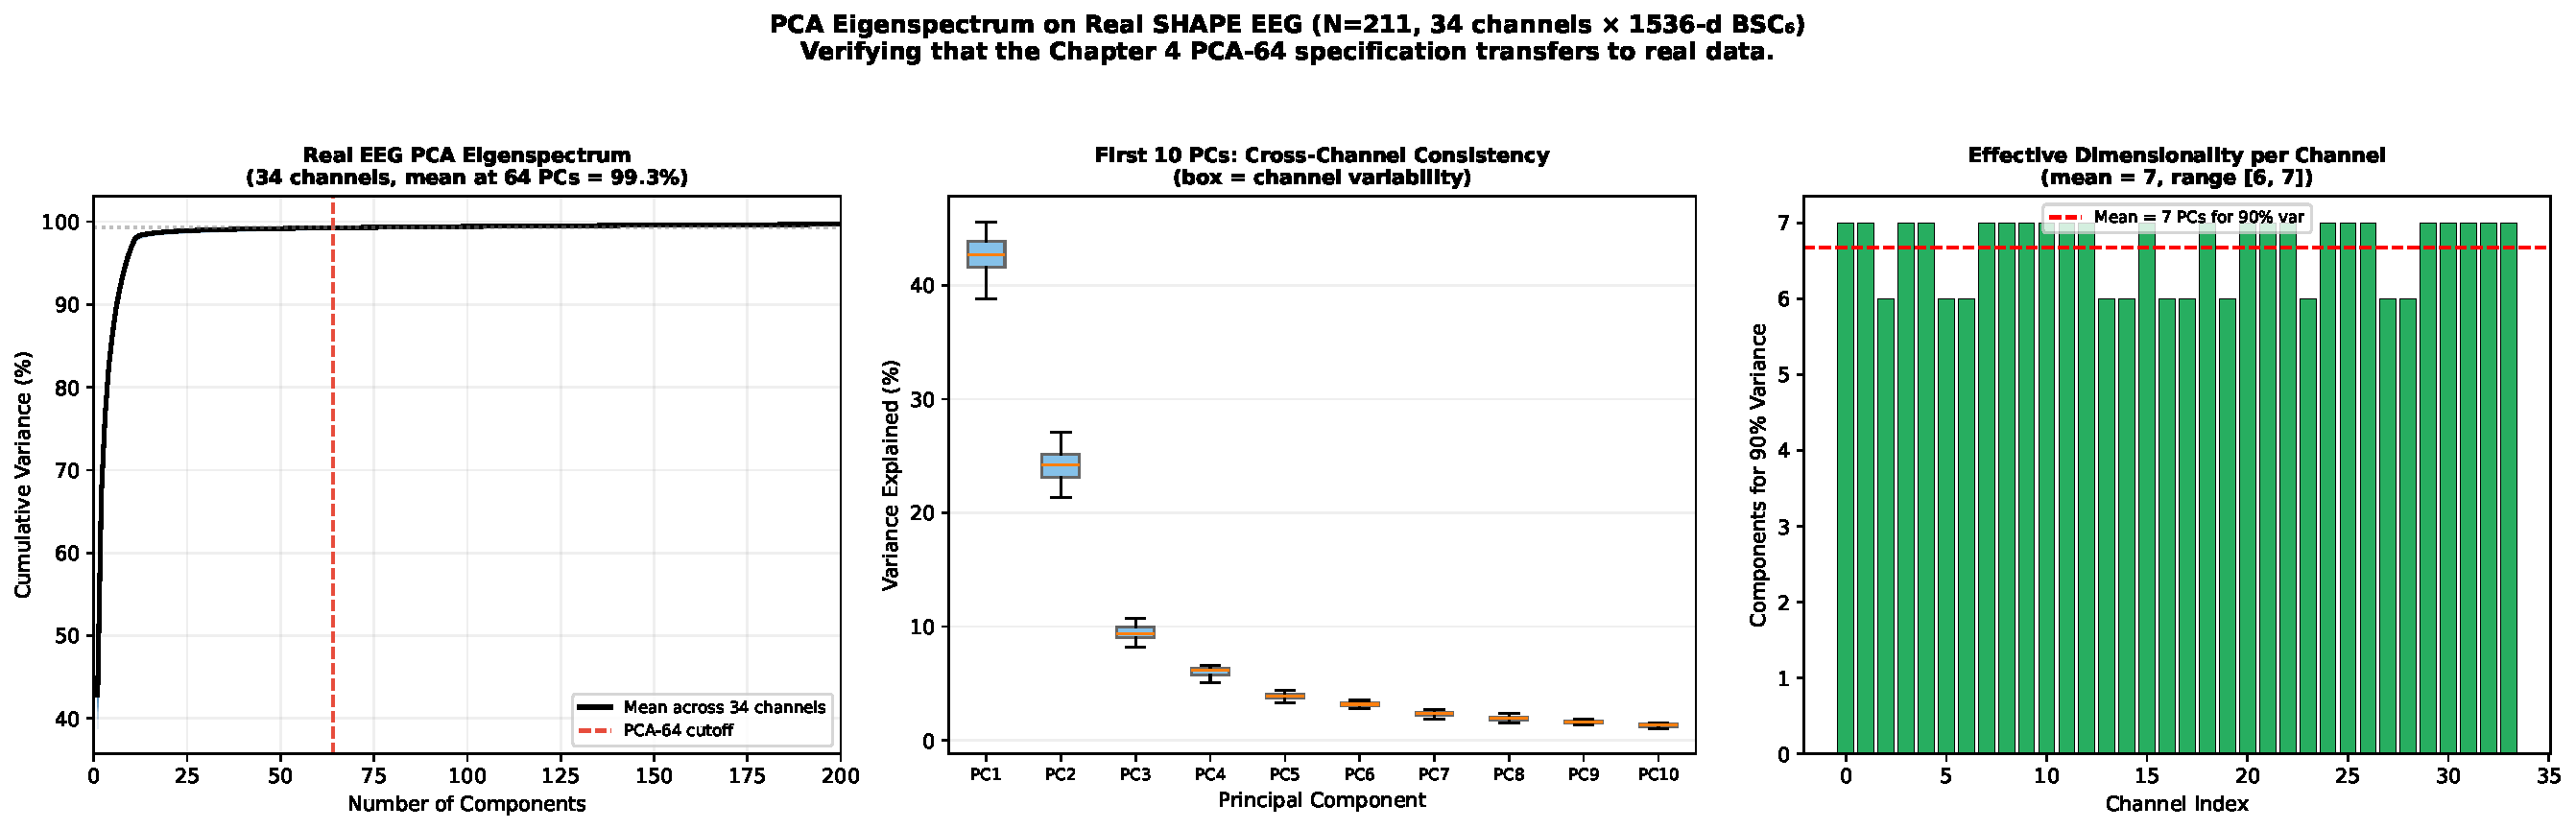
\includegraphics[width=\textwidth]{pictures/chGraphNeuralNetworks/obs09_real_pca_eigenspectrum.pdf}
    \caption{Archived per-channel PCA eigenspectra on SHAPE EEG. Left: cumulative sample-variance curves for all $34$ channels (gray) and their mean (black); 64 components retain $99.3\%$. Center: first ten eigenvalues. Right: six or seven per-channel components reach the $90\%$ sample-variance threshold. Separately fitted axes are not commensurate.}
    \label{fig:obs09_pca}
\end{figure}

\subsection{Feature Space Comparison: Band-Power vs Reservoir}

Figure~\ref{fig:obs10_features} compares the archived feature spaces produced by band-power extraction and reservoir processing. The two-dimensional projections show substantial overlap, and the displayed fold distributions summarize the earlier global-PCA pipeline. Because PCA was fitted before fold separation, the numerical comparison is descriptive and must be recomputed before it can support a performance claim.

\begin{figure}[H]
    \centering
    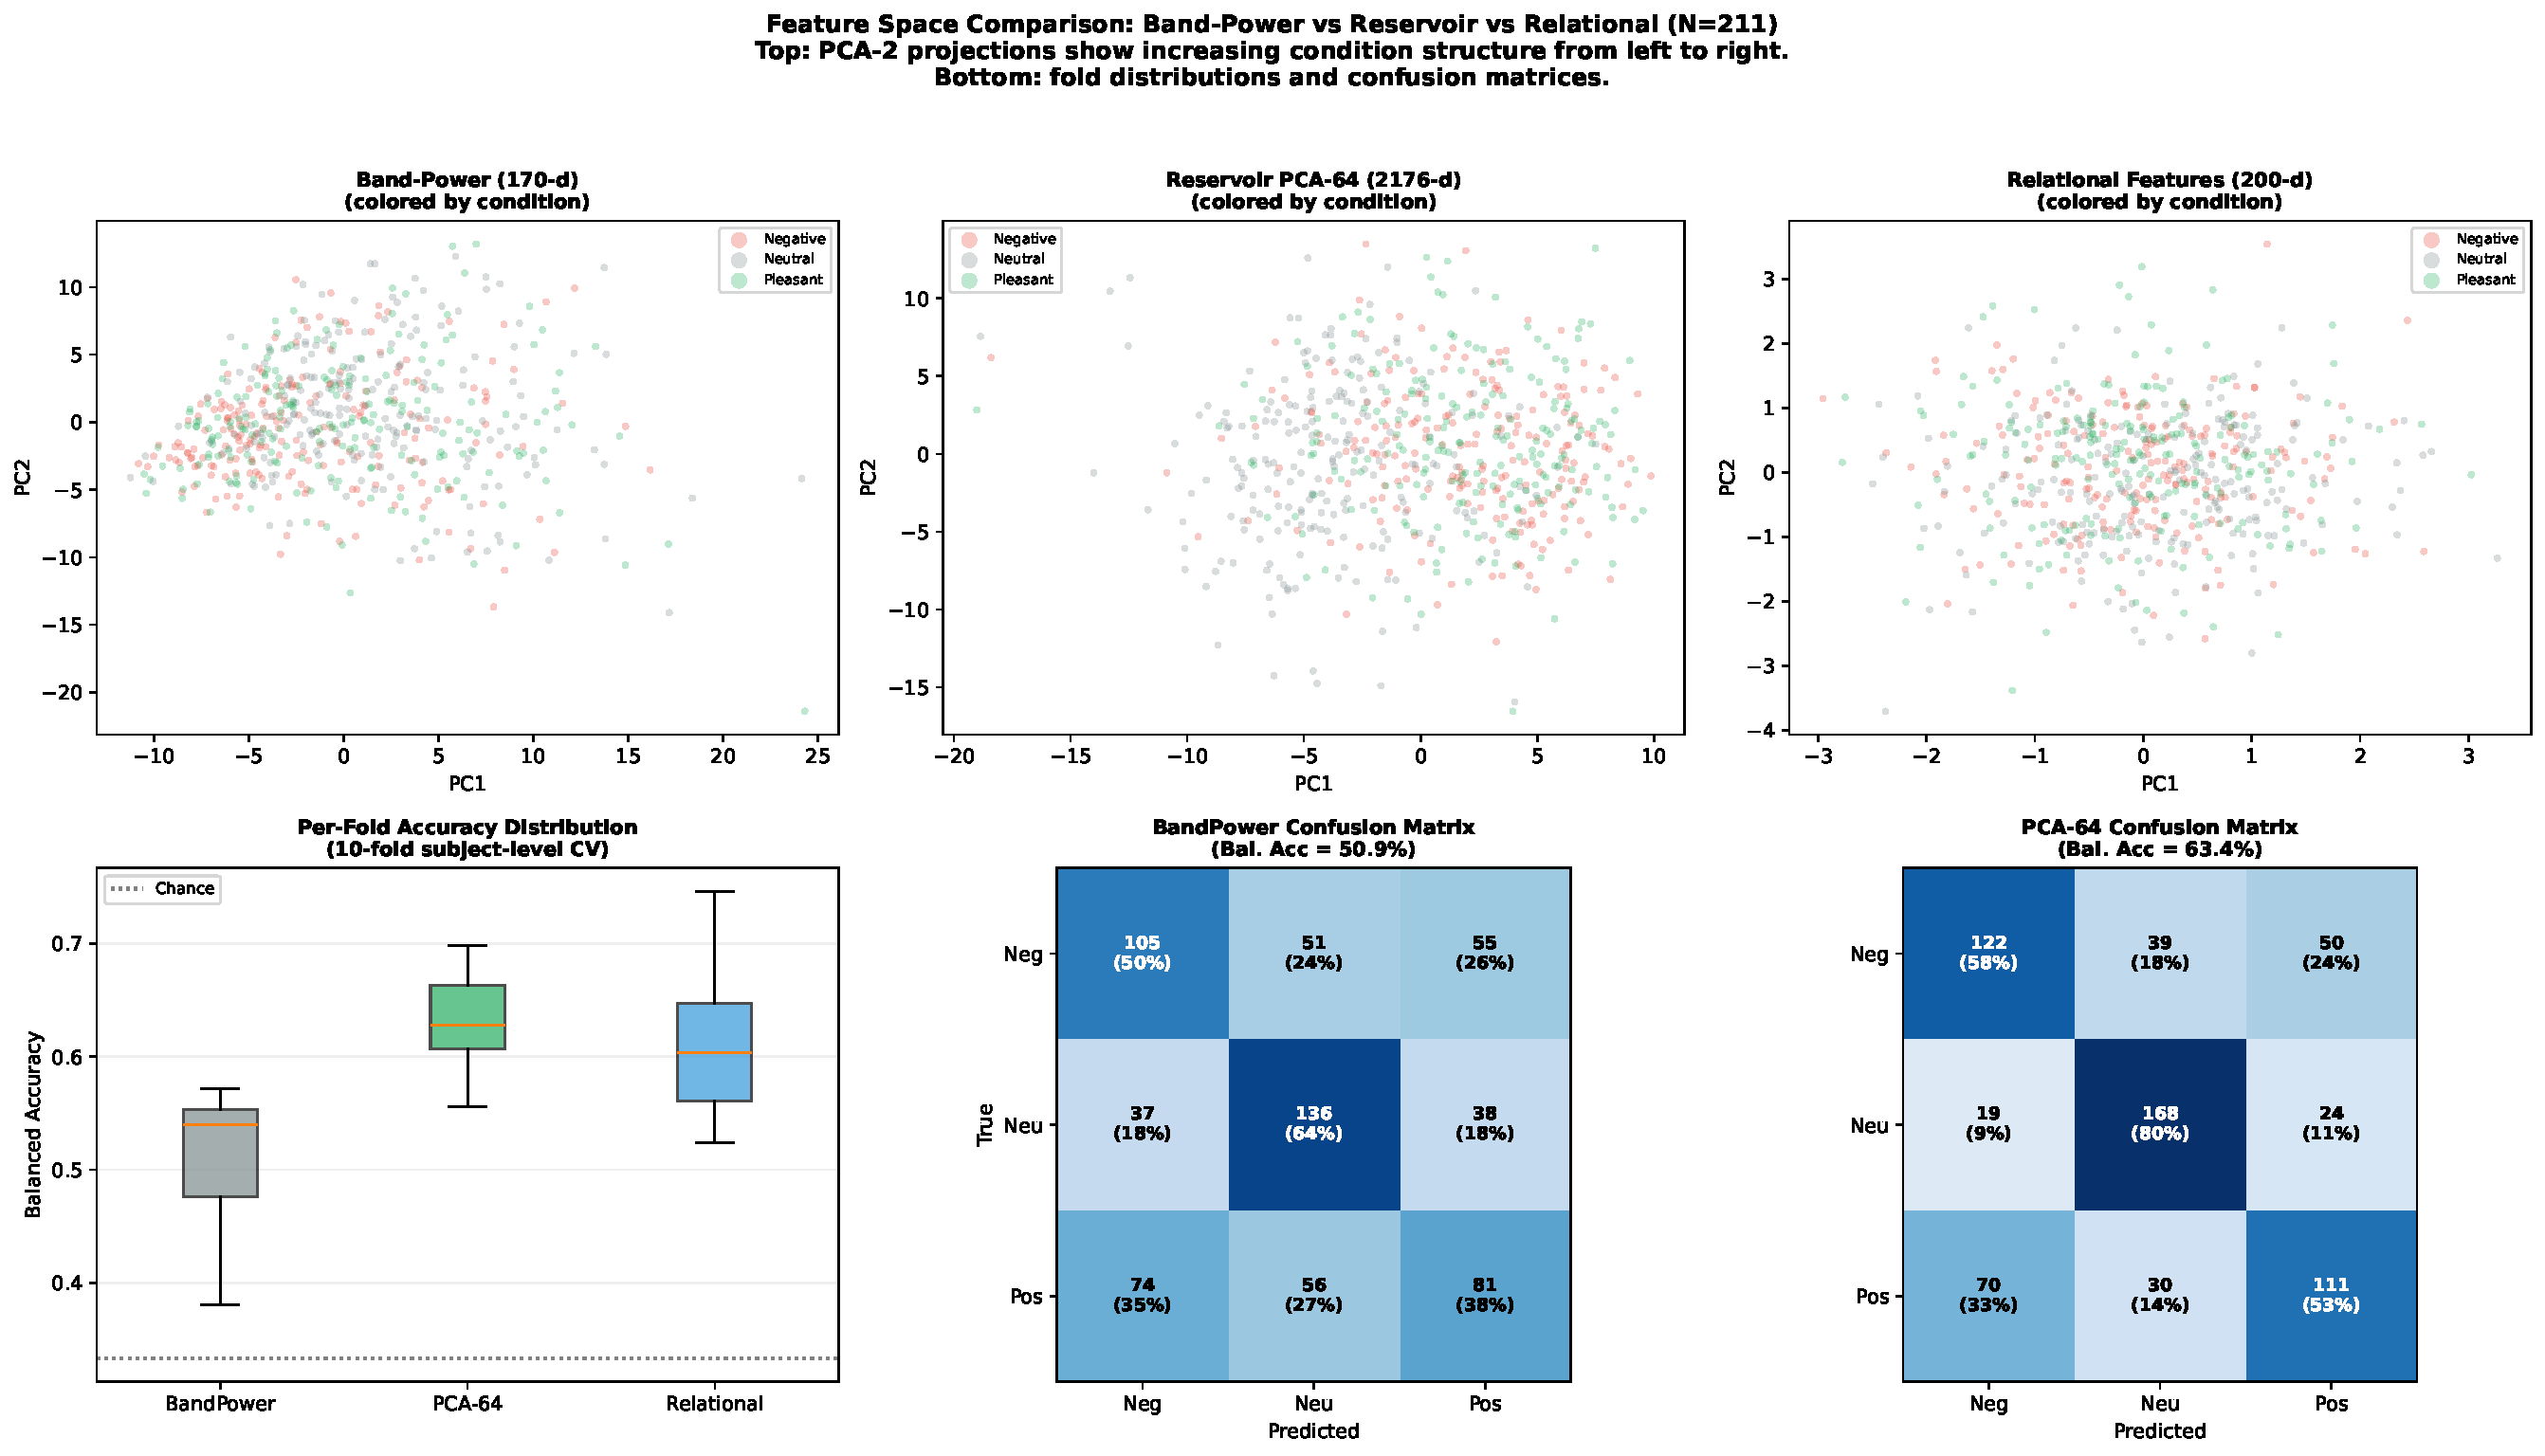
\includegraphics[width=\textwidth]{pictures/chGraphNeuralNetworks/obs10_feature_comparison.pdf}
    \caption{Archived feature-space comparison ($N=211$). The PCA-dependent results use global preprocessing and are descriptive legacy estimates.}
    \label{fig:obs10_features}
\end{figure}

\subsection{Condition-Dependent Graph Topology}

Figure~\ref{fig:obs06_conditions} examines how the archived similarity graphs change across emotional conditions. The three condition-average graphs appear similar at the $20\%$ density threshold, and the edge-difference distribution is centered near zero. The small displayed differences are descriptive; the noncommensurate per-channel PCA axes and lack of multiplicity-adjusted edge inference preclude a claim that a distributed physiological condition signal has been established.

\begin{figure}[H]
    \centering
    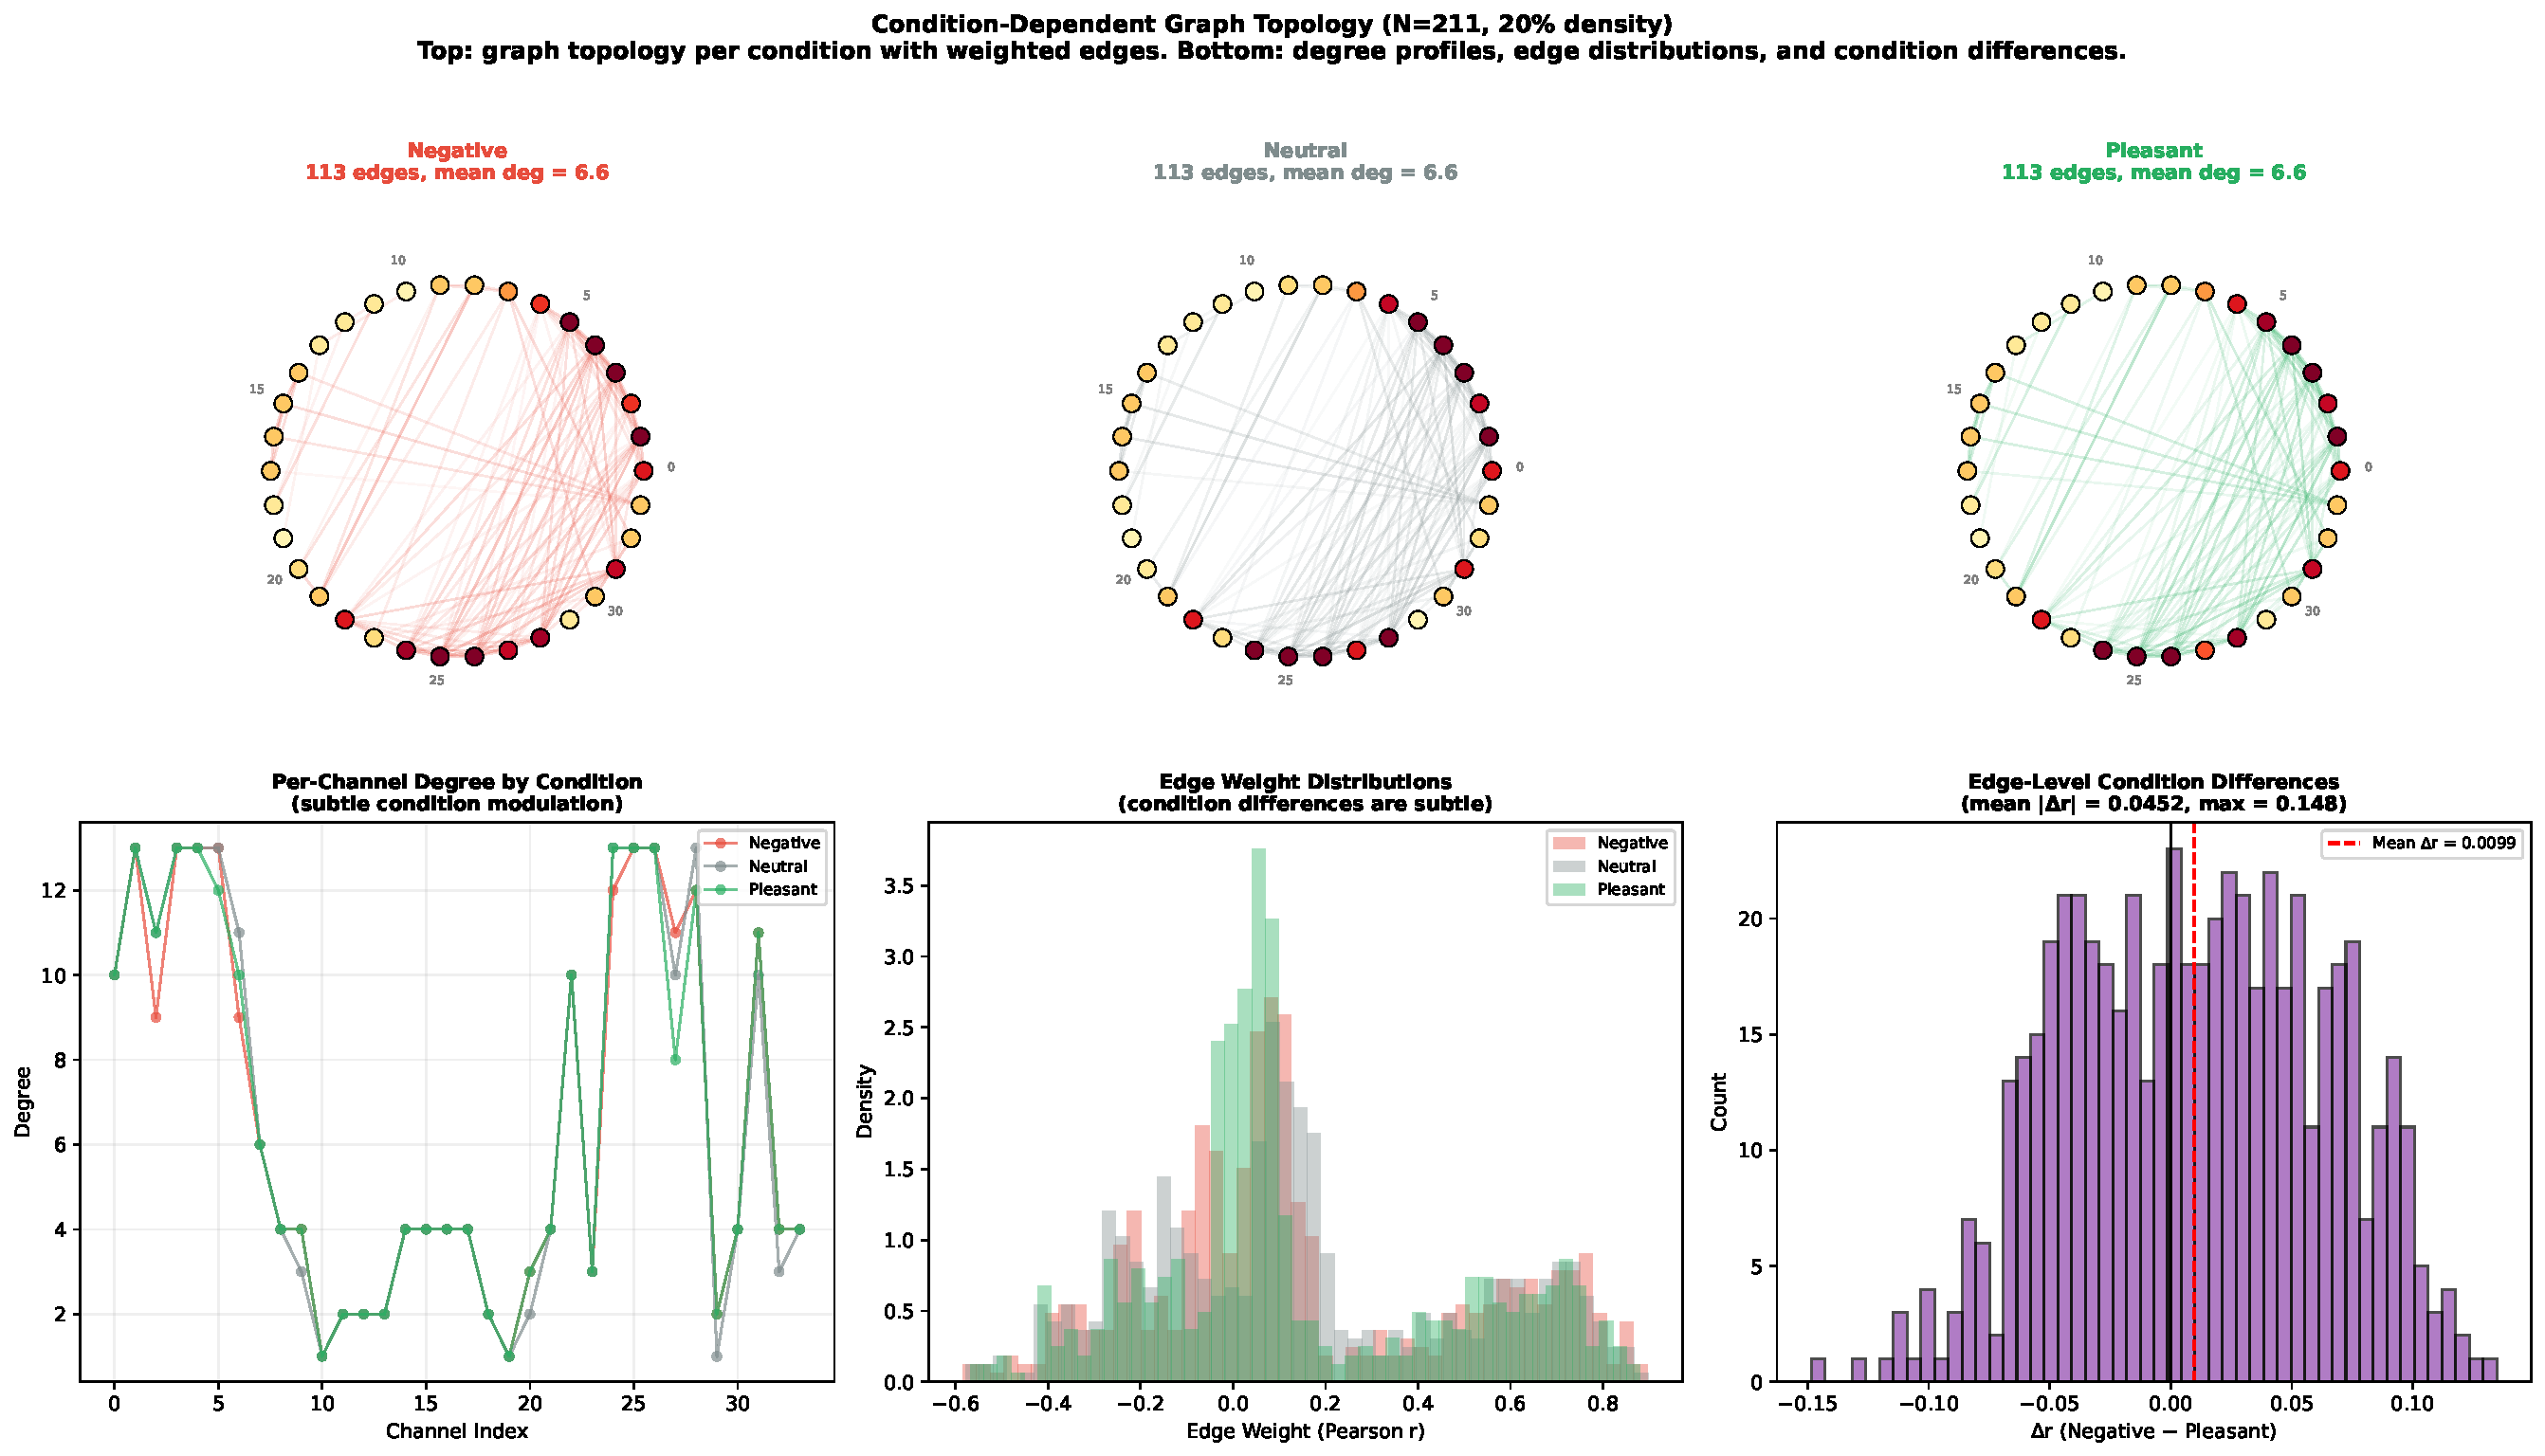
\includegraphics[width=\textwidth]{pictures/chGraphNeuralNetworks/obs06_condition_differences.pdf}
    \caption{Condition-dependent graph topology ($N = 211$). Top: per-condition graphs with weighted edges (node color $=$ degree). Bottom: degree profiles, edge weight distributions, and edge-level condition differences (mean $|\Delta r| = 0.045$).}
    \label{fig:obs06_conditions}
\end{figure}

\subsection{Graph Property Distributions Across Subjects}

Figure~\ref{fig:obs12_properties} summarizes five archived graph properties across the $211$ participants. Mean edge weight has coefficient of variation (CV) $0.22$, mean clustering CV $0.15$, global efficiency CV $0.10$, and degree heterogeneity CV $0.21$. Mean weight and efficiency have Spearman $\rho=0.84$, while degree heterogeneity has $|\rho|<0.15$ with the other displayed metrics. Low rank correlation does not establish statistical independence.

\begin{figure}[H]
    \centering
    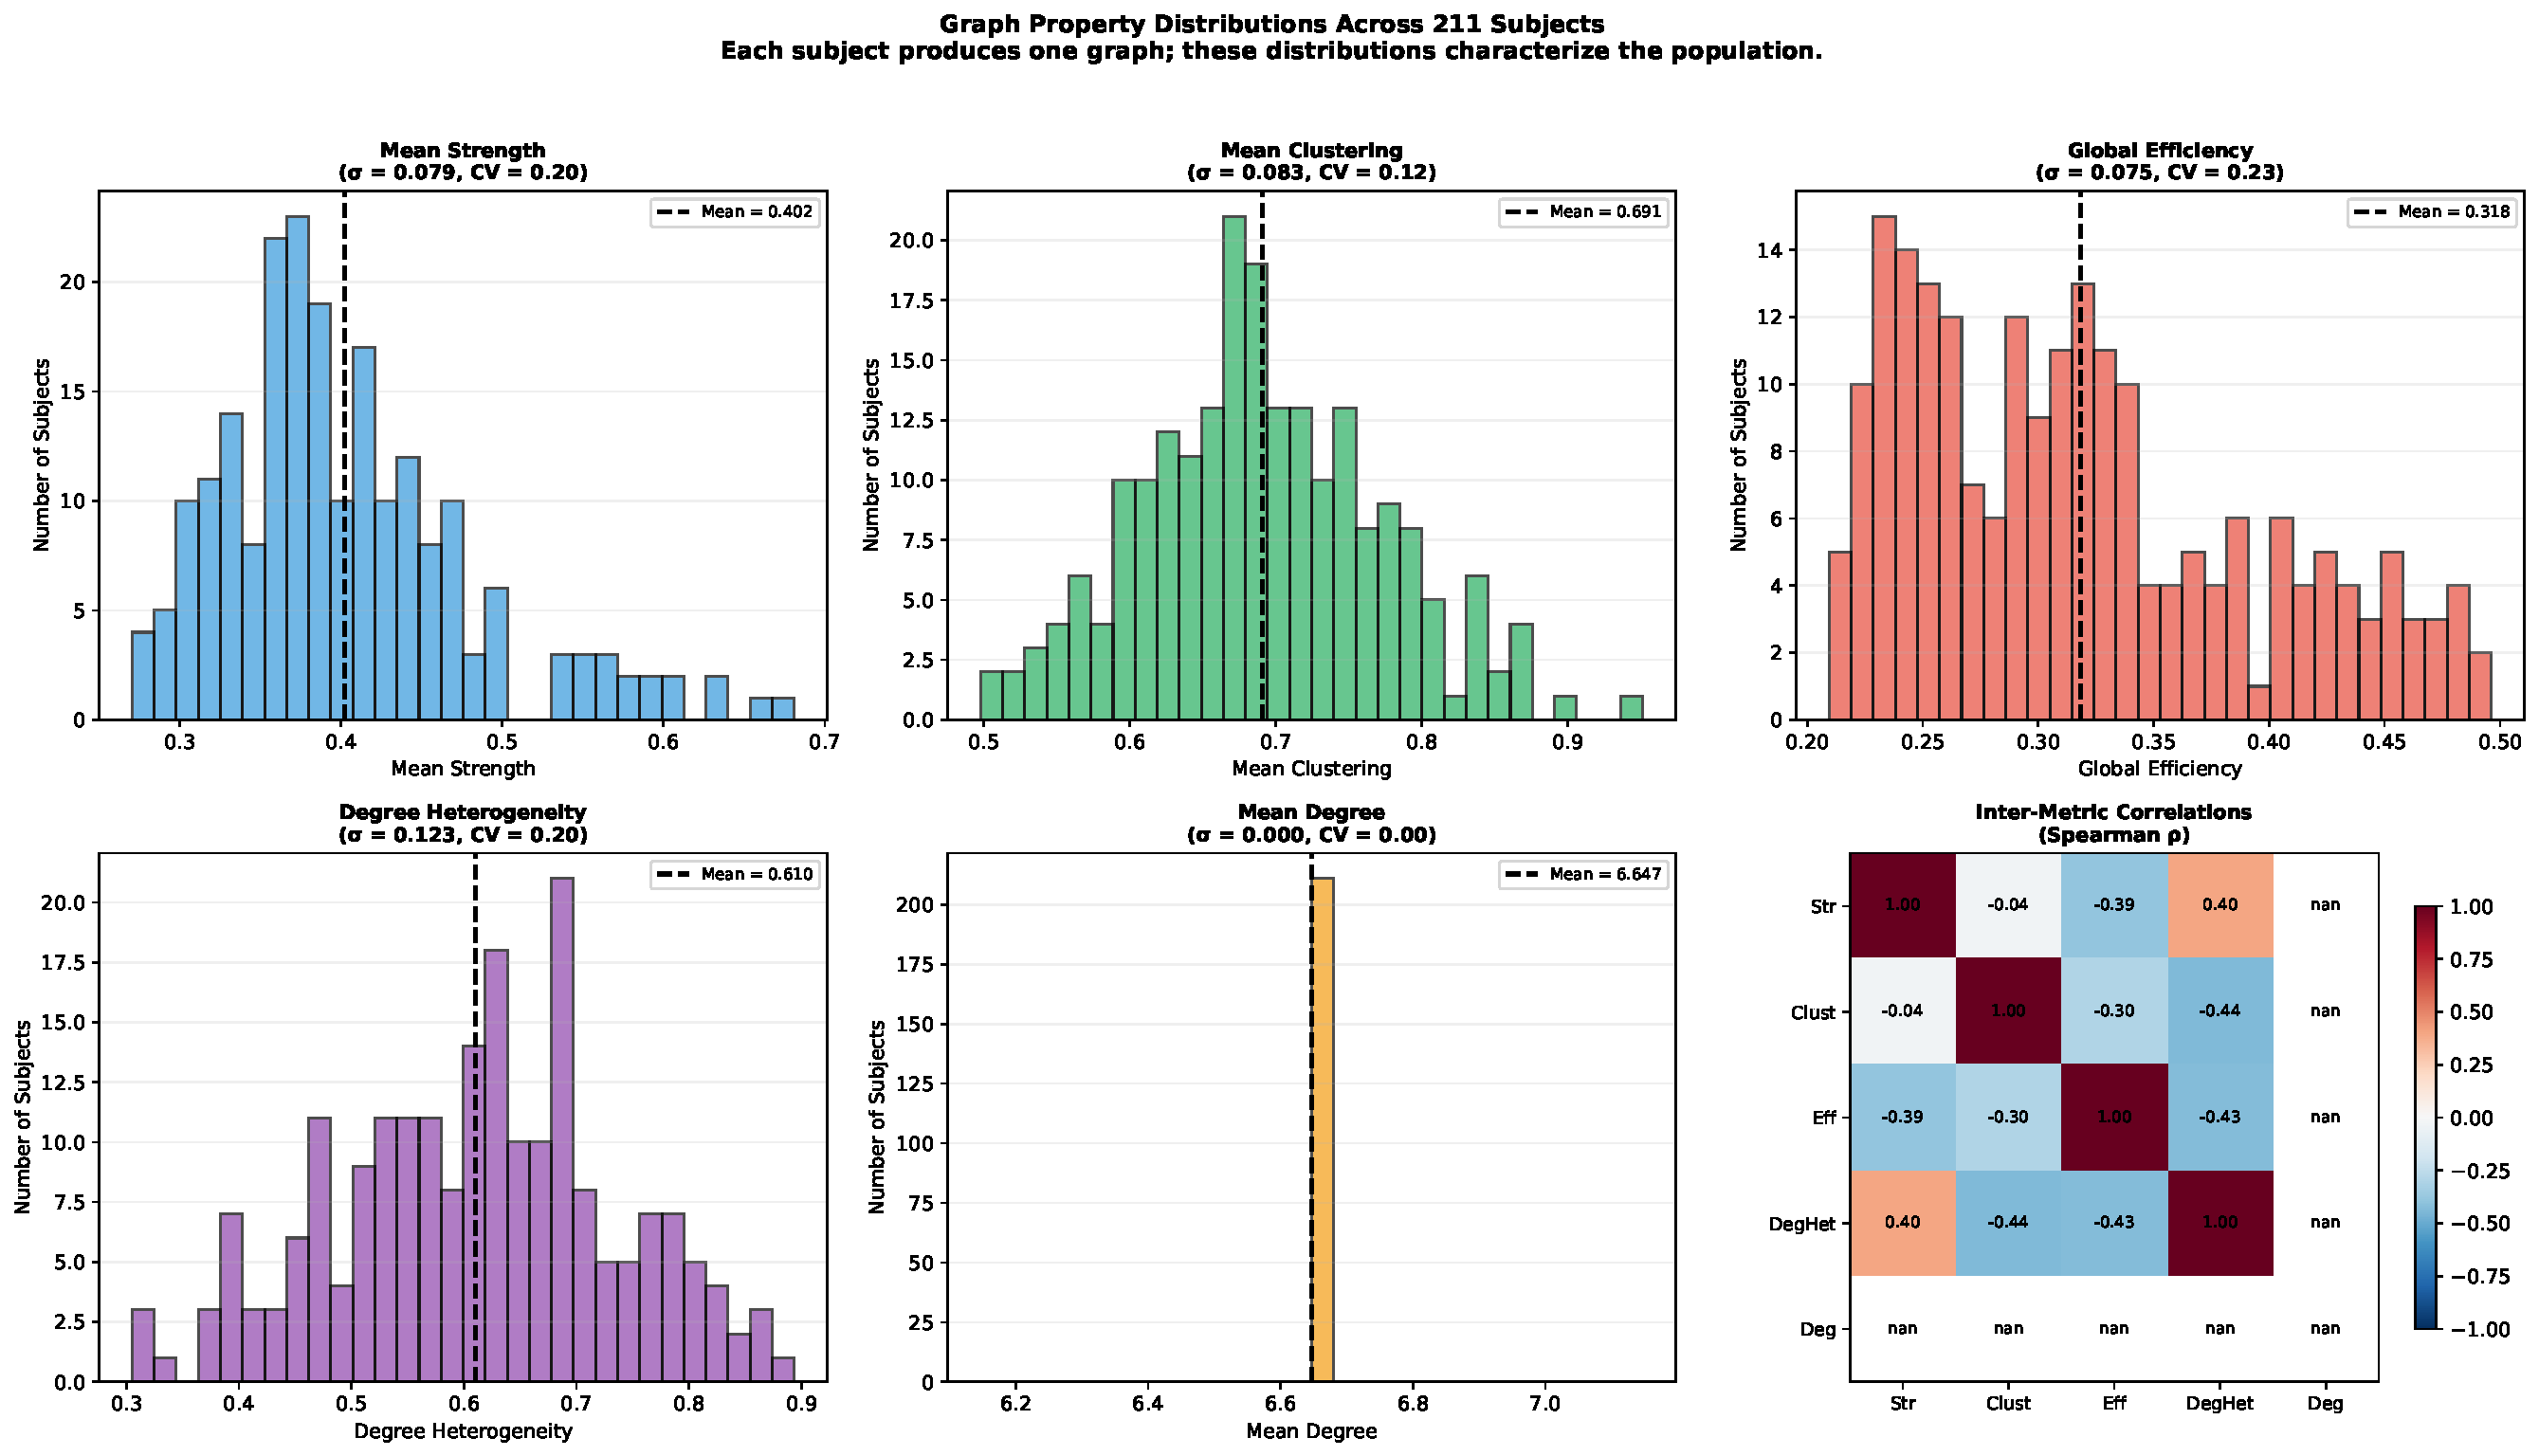
\includegraphics[width=\textwidth]{pictures/chGraphNeuralNetworks/obs12_graph_property_distributions.pdf}
    \caption{Archived graph-property distributions across $211$ participants, with sample means, standard deviations, CVs, and inter-metric Spearman correlations. Mean weight and efficiency have $\rho=0.84$; degree heterogeneity has weak displayed rank correlations with the other metrics.}
    \label{fig:obs12_properties}
\end{figure}

\subsection{Graph Propagation Smoothing Analysis}

Figure~\ref{fig:obs11_variance} illustrates smoothing for one archived graph construction. Inter-channel variance decreases by $33\%$ after two layers and mean cosine similarity increases. These quantities show homogenization, but do not identify how much of the removed variance was discriminative or provide a general criterion for other sensor graphs.

\begin{figure}[H]
    \centering
    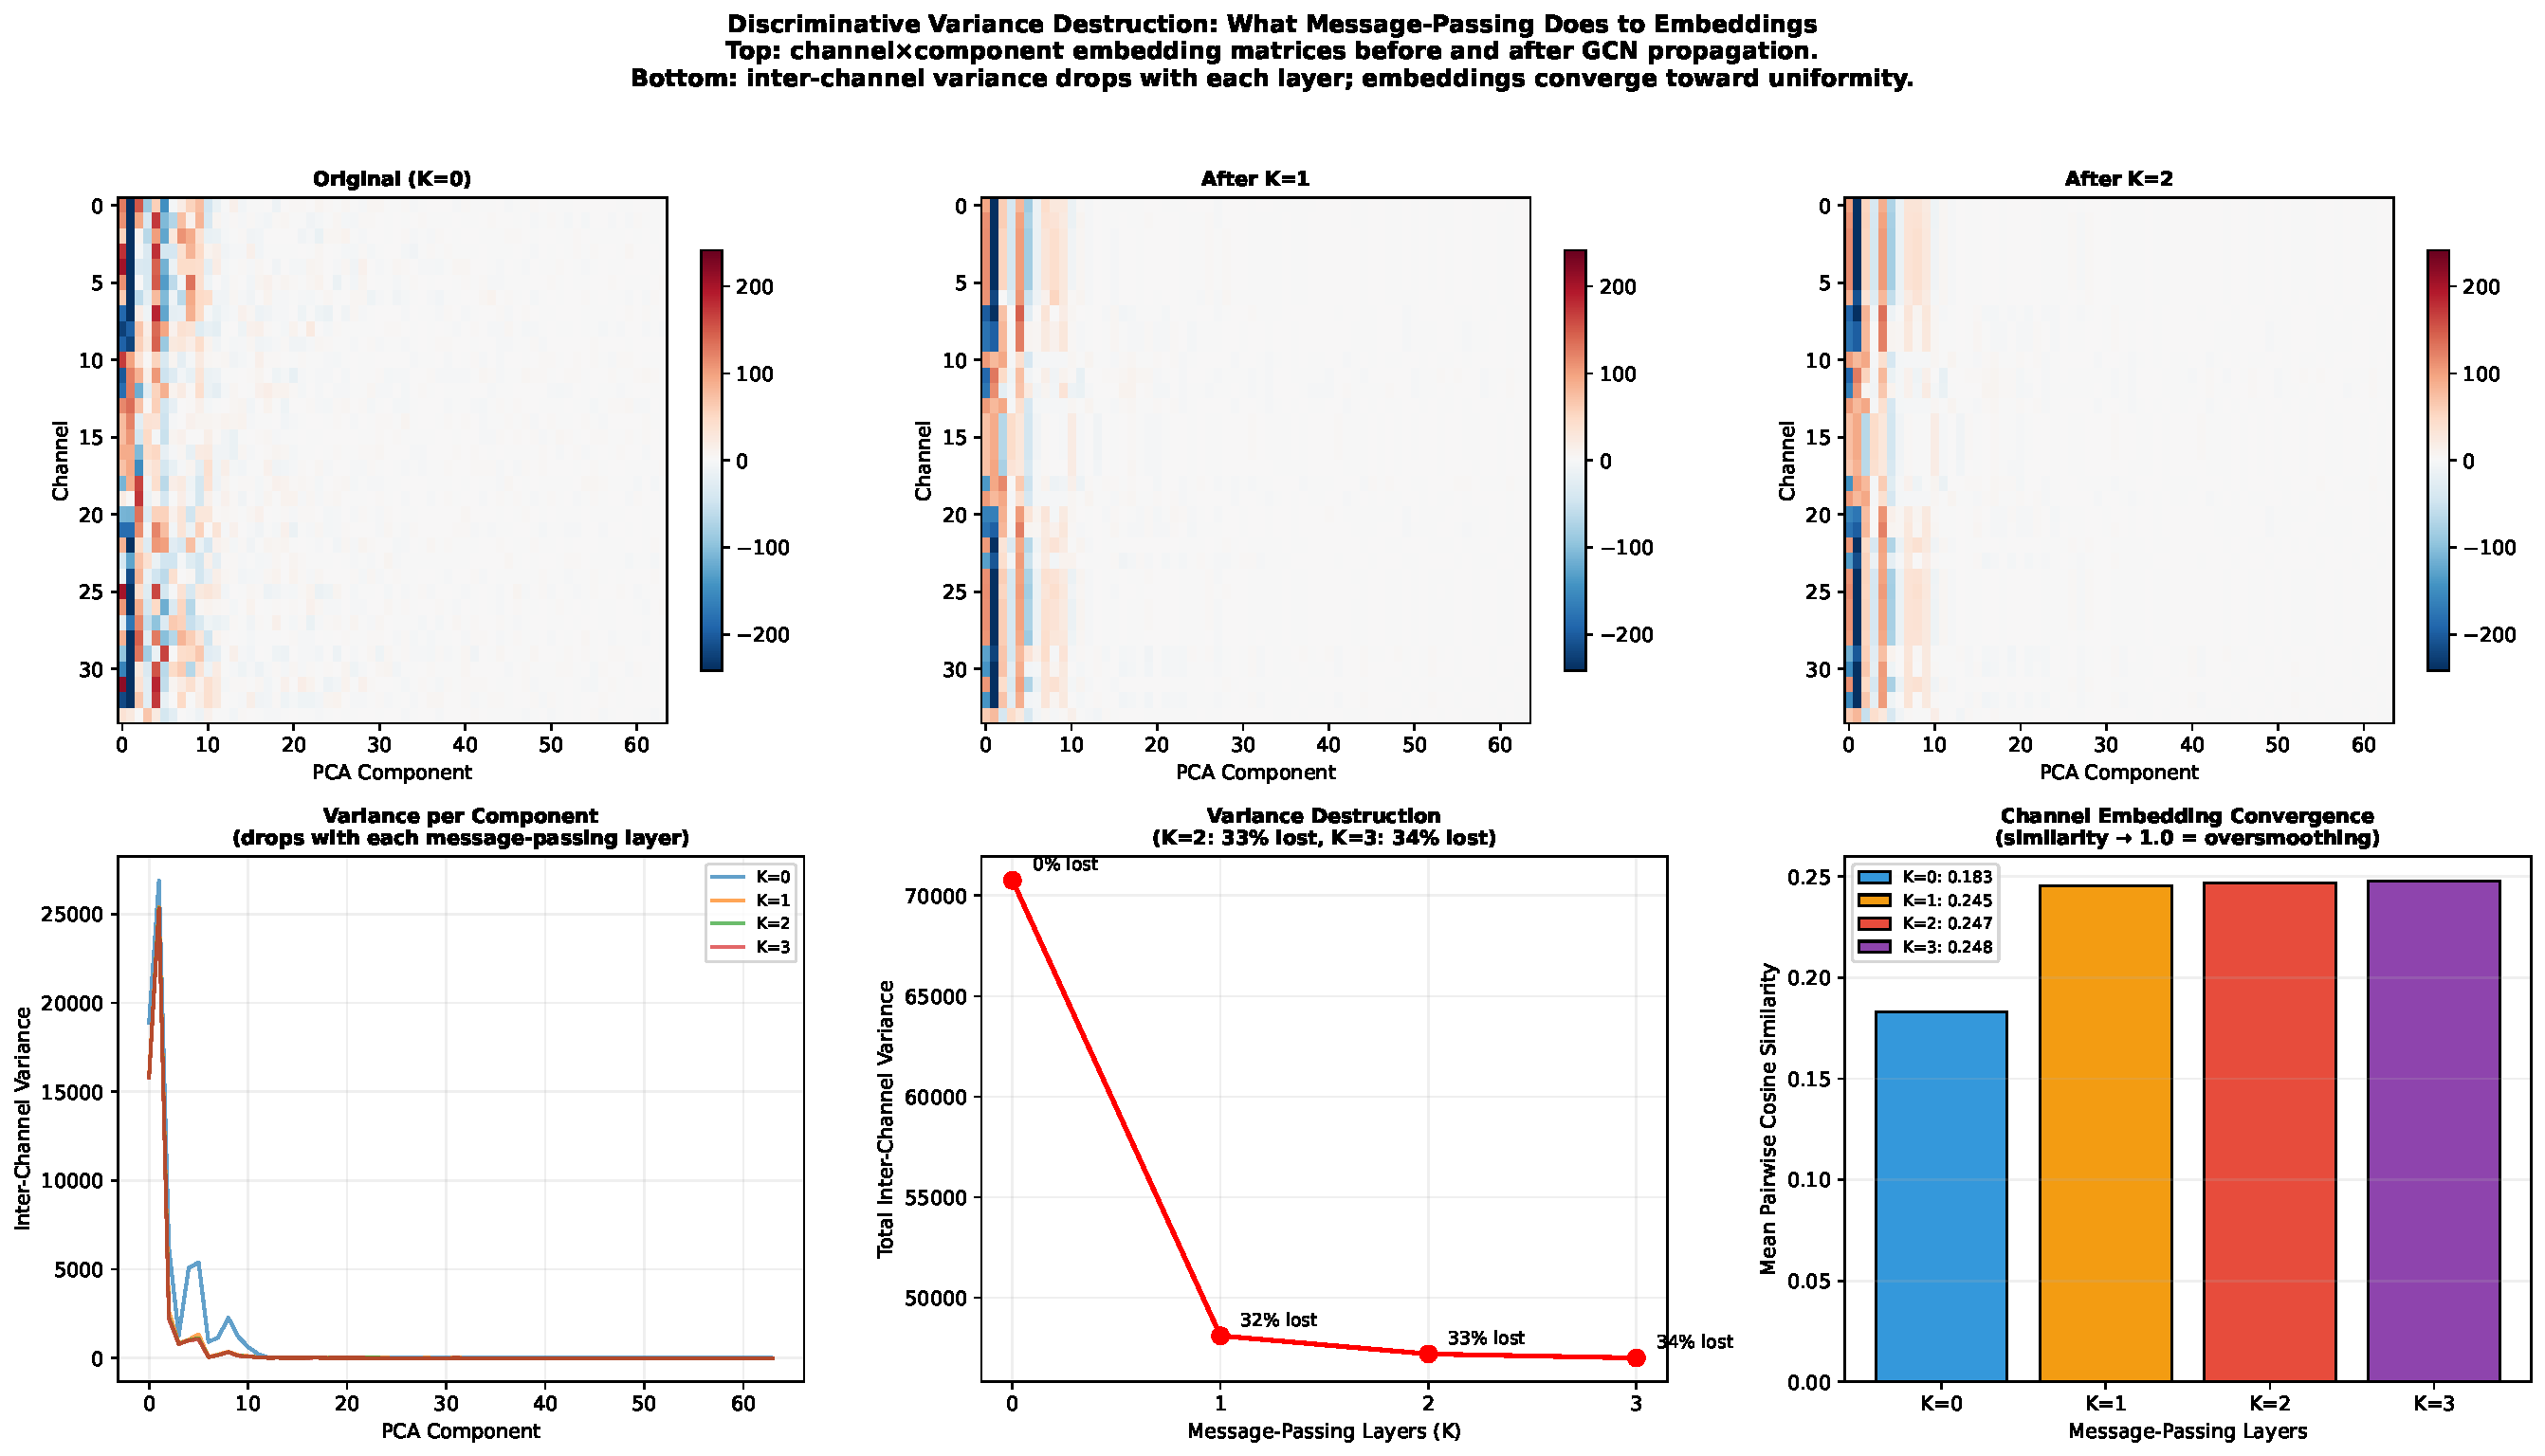
\includegraphics[width=\textwidth]{pictures/chGraphNeuralNetworks/obs11_variance_destruction.pdf}
    \caption{Archived propagation-smoothing illustration. Inter-channel variance decreases and pairwise cosine similarity increases for the displayed construction; no general regime boundary is inferred.}
    \label{fig:obs11_variance}
\end{figure}


\section{Classification Experiments}
\label{sec:ch5_classification}

\subsection{Protocol}

The archived experiments target three-way emotion discrimination ($211$ observations per class) with $10$ subject-grouped folds, so no participant appears in both training and test partitions. However, PCA was fitted before the fold split; subject grouping therefore prevents direct row overlap but does not make PCA-dependent estimates fully held out.

\subsection{Baseline Methods}

Three archived baselines are compared in Table~\ref{tab:baselines}.

\textbf{M1: Band-Power + SVM.} Conventional spectral features ($170$ dimensions) classified by RBF-SVM. No reservoir, no graph.

\textbf{M2: PCA-64 Concatenation + SVM.} The $34 \times 64 = 2{,}176$-dimensional concatenation of all channel embeddings. Uses the reservoir but ignores inter-channel structure.

\textbf{M3: Pairwise Relational Features + SVM.} The $561$ channel-pair embedding differences, PCA-reduced to $200$ dimensions. Graph-informed but without message-passing.

\begin{table}[t]
\centering
\caption{Archived baseline estimates ($N=211$, $633$ observations, 10 subject-grouped folds). PCA-dependent values use global preprocessing and are not unbiased held-out estimates.}
\label{tab:baselines}
\begin{tabular}{llccc}
\hline
\textbf{Method} & \textbf{Features} & \textbf{Dim} & \textbf{Bal.\ Acc.} & \textbf{MCC} \\
\hline
M1: BandPower + SVM & Spectral power & $170$ & $50.9 \pm 6.3\%$ & $0.265$ \\
\textbf{M2: PCA-64 + SVM} & \textbf{Reservoir concat} & $\mathbf{2{,}176}$ & $\mathbf{63.4 \pm 4.4\%}$ & $\mathbf{0.457}$ \\
M3: Relational + SVM & Pairwise diffs & $200$ & $61.8 \pm 7.0\%$ & $0.437$ \\
\hline
\end{tabular}
\end{table}

The displayed M2 estimate is $63.4\%$, $12.5$ percentage points above M1 and $1.6$ points above M3. These are legacy point-estimate differences; global PCA, overlapping nested samples, and the absence of a nested model comparison prevent causal claims about which representation benefits from additional data.

\subsection{Message-Passing GNN Experiments}

Three architectures were evaluated as five-seed ensembles with concatenated graph readouts classified by SVM (Figure~\ref{fig:gnn_comparison}, Table~\ref{tab:gnn_results}). The archived Wilcoxon tests treat ten cross-validation folds as paired observations. Fold scores are dependent because training sets overlap, and PCA was global, so those $p$ values are retained for provenance but not interpreted as confirmatory significance tests.

\begin{figure}[H]
    \centering
    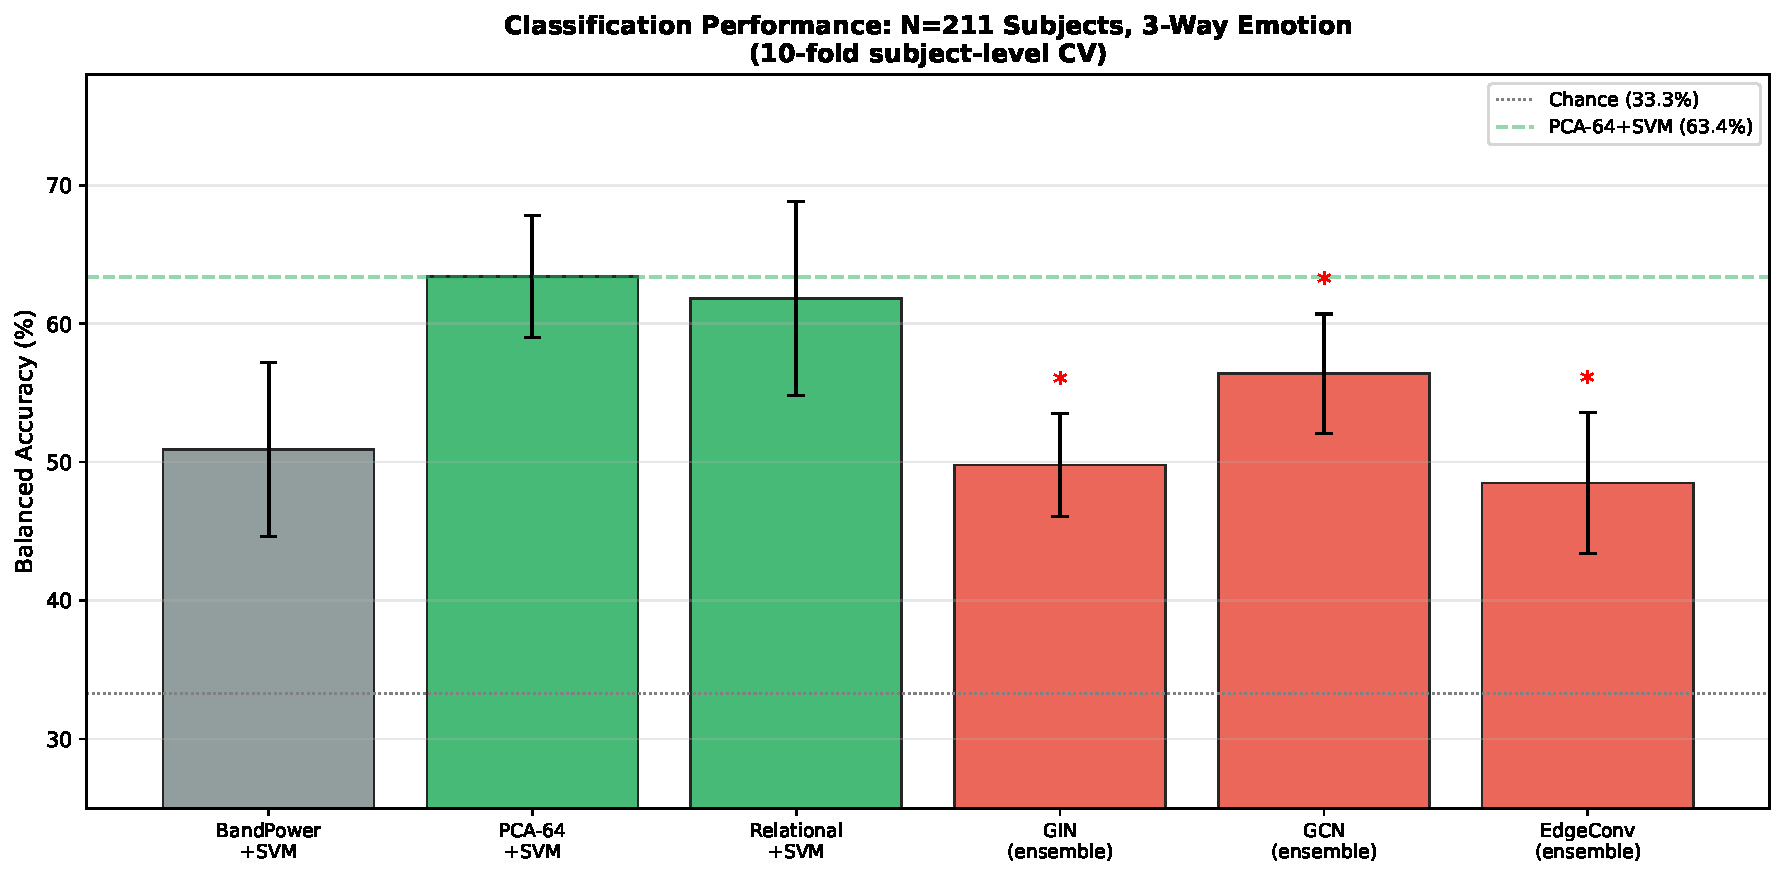
\includegraphics[width=\textwidth]{pictures/chGraphNeuralNetworks/fig_05_gnn_comparison_211.pdf}
    \caption{Archived classification comparison at $N=211$. Asterisks show the original fold-wise tests, which use dependent cross-validation scores and are not interpreted as confirmatory. Chance $=33.3\%$.}
    \label{fig:gnn_comparison}
\end{figure}

\begin{table}[t]
\centering
\caption{Archived message-passing estimates at $N=211$. The displayed $p$ values come from dependent fold-wise comparisons and do not identify a general regime boundary.}
\label{tab:gnn_results}
\begin{tabular}{lcccc}
\hline
\textbf{Architecture} & \textbf{Bal.\ Acc.} & \textbf{MCC} & \textbf{$p$ vs.\ M2} & \textbf{$N\!=\!115$ result} \\
\hline
GIN (5-seed) & $49.8 \pm 3.7\%$ & $0.250$ & $0.004$ & $51.6\%$ \\
GCN (5-seed) & $56.4 \pm 4.3\%$ & $0.349$ & $0.035$ &, \\
EdgeConv (5-seed) & $48.5 \pm 5.1\%$ & $0.234$ & $0.006$ & $53.0\%$ \\
\hline
\end{tabular}
\end{table}

The $N=115$ observations form a subset of the $N=211$ cohort and therefore do not constitute an independent replication. In the archived runs, GIN and EdgeConv did not improve as the larger subset was used, whereas the concatenated baseline did. Differences in training stochasticity, preprocessing, and overlapping samples prevent attributing that pattern to a structural property of EEG graphs. The result is limited to the tested implementations and this cohort.


\subsection{Conventional End-to-End Baselines}

The preceding sections compare ARSPI-Net against spectral features and graph-propagation variants. A natural question is how the reservoir embedding compares against standard trainable models operating directly on the raw multichannel EEG. Table~\ref{tab:conventional_baselines} presents this comparison using the same $10$-fold subject-level cross-validation protocol.

\begin{table}[H]
\centering
\caption{Archived baseline comparison ($N=211$, $633$ observations, 10 subject-grouped folds). Deep models use five-seed ensembles. Centered columns use all three held-out observations per subject and therefore estimate a transductive panel task. PCA-dependent values also use global preprocessing.}
\label{tab:conventional_baselines}
\small
\begin{tabularx}{\textwidth}{@{}>{\raggedright\arraybackslash}Xlcccc@{}}
\hline
\textbf{Method} & \textbf{Input} & \textbf{Dim} & \textbf{Uncent.} & \textbf{Centered} & \textbf{$\Delta$} \\
\hline
\multicolumn{6}{l}{\textit{Spectral features}} \\
BandPower + SVM & Spectral & $170$ & $47.7 \pm 5.1\%$ & $61.0 \pm 6.0\%$ & $+13.3$ \\
\hline
\multicolumn{6}{l}{\textit{Raw EEG, linear readout}} \\
Raw EEG PCA-200 + LogReg & Raw EEG & $200$ & $64.9 \pm 5.0\%$ & $86.4 \pm 4.1\%$ & $+21.5$ \\
Raw EEG (full) + LogReg & Raw EEG & $8{,}704$ & $70.5 \pm 3.0\%$ & $88.4 \pm 2.1\%$ & $+17.9$ \\
\hline
\multicolumn{6}{l}{\textit{Trained deep architectures}} \\
LSTM (bidir, 64h) & Raw EEG & $34 \times 256$ & $58.0 \pm 5.5\%$ & $71.1 \pm 6.8\%$ & $+13.1$ \\
GRU (bidir, 64h) & Raw EEG & $34 \times 256$ & $59.9 \pm 6.4\%$ & $78.4 \pm 3.5\%$ & $+18.5$ \\
\textbf{EEGNet} & \textbf{Raw EEG} & $\mathbf{34 \times 256}$ & $\mathbf{72.0 \pm 4.9\%}$ & $\mathbf{89.1 \pm 3.1\%}$ & $\mathbf{+17.1}$ \\
\hline
\multicolumn{6}{l}{\textit{ARSPI-Net reservoir (fixed recurrent stage)}} \\
Reservoir + LogReg & BSC$_6$/PCA & $2{,}176$ & $59.4 \pm 3.6\%$ & $78.8 \pm 3.4\%$ & $+19.4$ \\
\hline
\end{tabularx}
\end{table}

\begin{figure}[t]
\centering
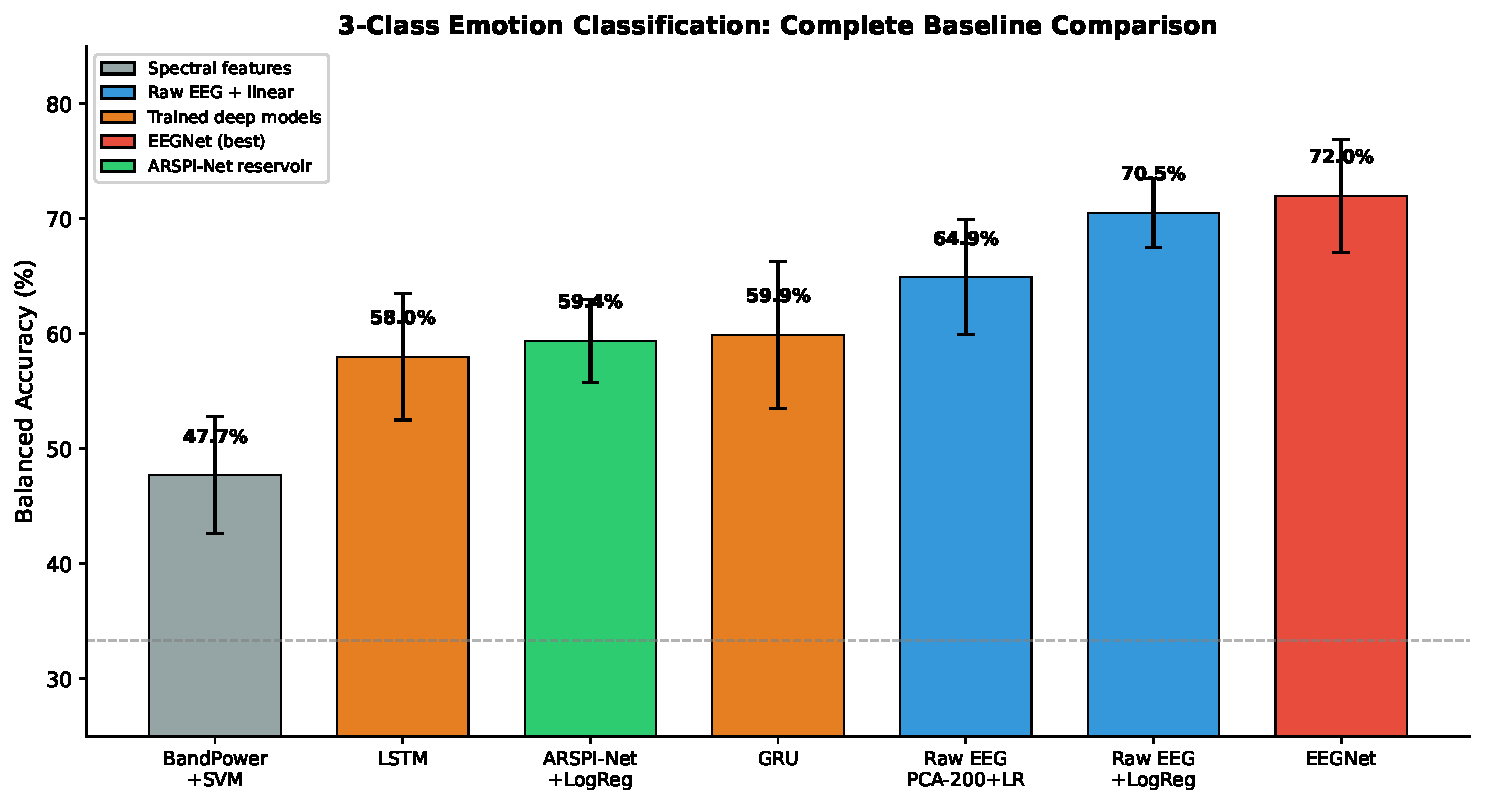
\includegraphics[width=0.85\textwidth]{pictures/chGraphNeuralNetworks/fig_baseline_comparison.pdf}
\caption{Archived baseline comparison on the three-class SHAPE task ($N = 211$, $10$ subject-grouped folds). Right bars use per-subject panel centering. PCA-dependent values were produced by the earlier global-PCA pipeline and are descriptive legacy estimates. Chance $= 33.3\%$.}
\label{fig:baseline_comparison}
\end{figure}

The archived table shows the highest uncentered point estimate for EEGNet ($72.0\%\pm4.9\%$). The reservoir estimate is close to the displayed GRU and LSTM estimates, while the full raw-EEG linear model is higher. The comparison uses different optimization procedures and feature pipelines, so the gaps cannot be attributed to a particular memory--nonlinearity tradeoff.

Panel centering increases every displayed estimate. Because this operation changes the prediction task by using all three held-out observations from each participant, the increase should not be called recovery from underperformance or compared with single-observation deployment. The reservoir exposes specified intermediate variables, but the table does not measure explanation fidelity or compare what alternative models could expose.

\paragraph{Uncertainty and estimand.} The archived fold-wise intervals for centering gains exclude zero for the reported models. Those folds are not independent experimental replications, however, and a post-hoc minimum-detectable-effect calculation does not validate the estimated gains. More importantly, the centered analysis uses a different, transductive estimand because every held-out subject contributes all three condition observations to that subject's normalization. Its values are not directly comparable to single-observation deployment accuracy.

\subsubsection{Interpretation: Inspectable Intermediate Measurements}

The complete baseline table (Table~\ref{tab:conventional_baselines}) distinguishes predictive performance from representation analysis. EEGNet achieves the highest centered accuracy ($89.1\%$), while raw EEG with a linear readout reaches $88.4\%$. Neither baseline is evaluated with the same predefined dynamical and topological descriptors used for ARSPI-Net, so the comparison concerns the analyses performed here rather than the inherent interpretability of every possible implementation.

The pipeline produces a classification output and specified intermediate summaries. Fixed recurrent weights make the transformation repeatable for a saved initialization and parameter set. The spike count has a defined computational unit; PCA coordinates and graph summaries are dimensionless model quantities. Explicit construction improves traceability but does not supply clinical meaning.

The roughly ten-point difference between the displayed centered raw-EEG and reservoir estimates cannot be converted into an information-theoretic quantity. It may reflect compression, model capacity, optimization, preprocessing, or sampling. The reservoir was analyzed with a predefined set of intermediate summaries; the comparison did not test whether analogous summaries or attribution methods could be constructed for the raw-EEG model.


\section{Representation Geometry: Variance Decomposition and Signal Detection}
\label{sec:ch5_variance}

The classification results raise a question motivated by signal detection theory: what is the structure of the representation space in which the classifier operates, and what are the dominant sources of variance?

\subsection{Variance Decomposition}

An archived one-way decomposition of the $2{,}176$-dimensional concatenated embedding assigns a larger sample sum-of-squares fraction to participant than to condition (Figure~\ref{fig:exp01_variance}). Because the transformation was fitted globally, the result is a property of that in-sample representation rather than a population estimate of latent subject identity.

\begin{figure}[H]
    \centering
    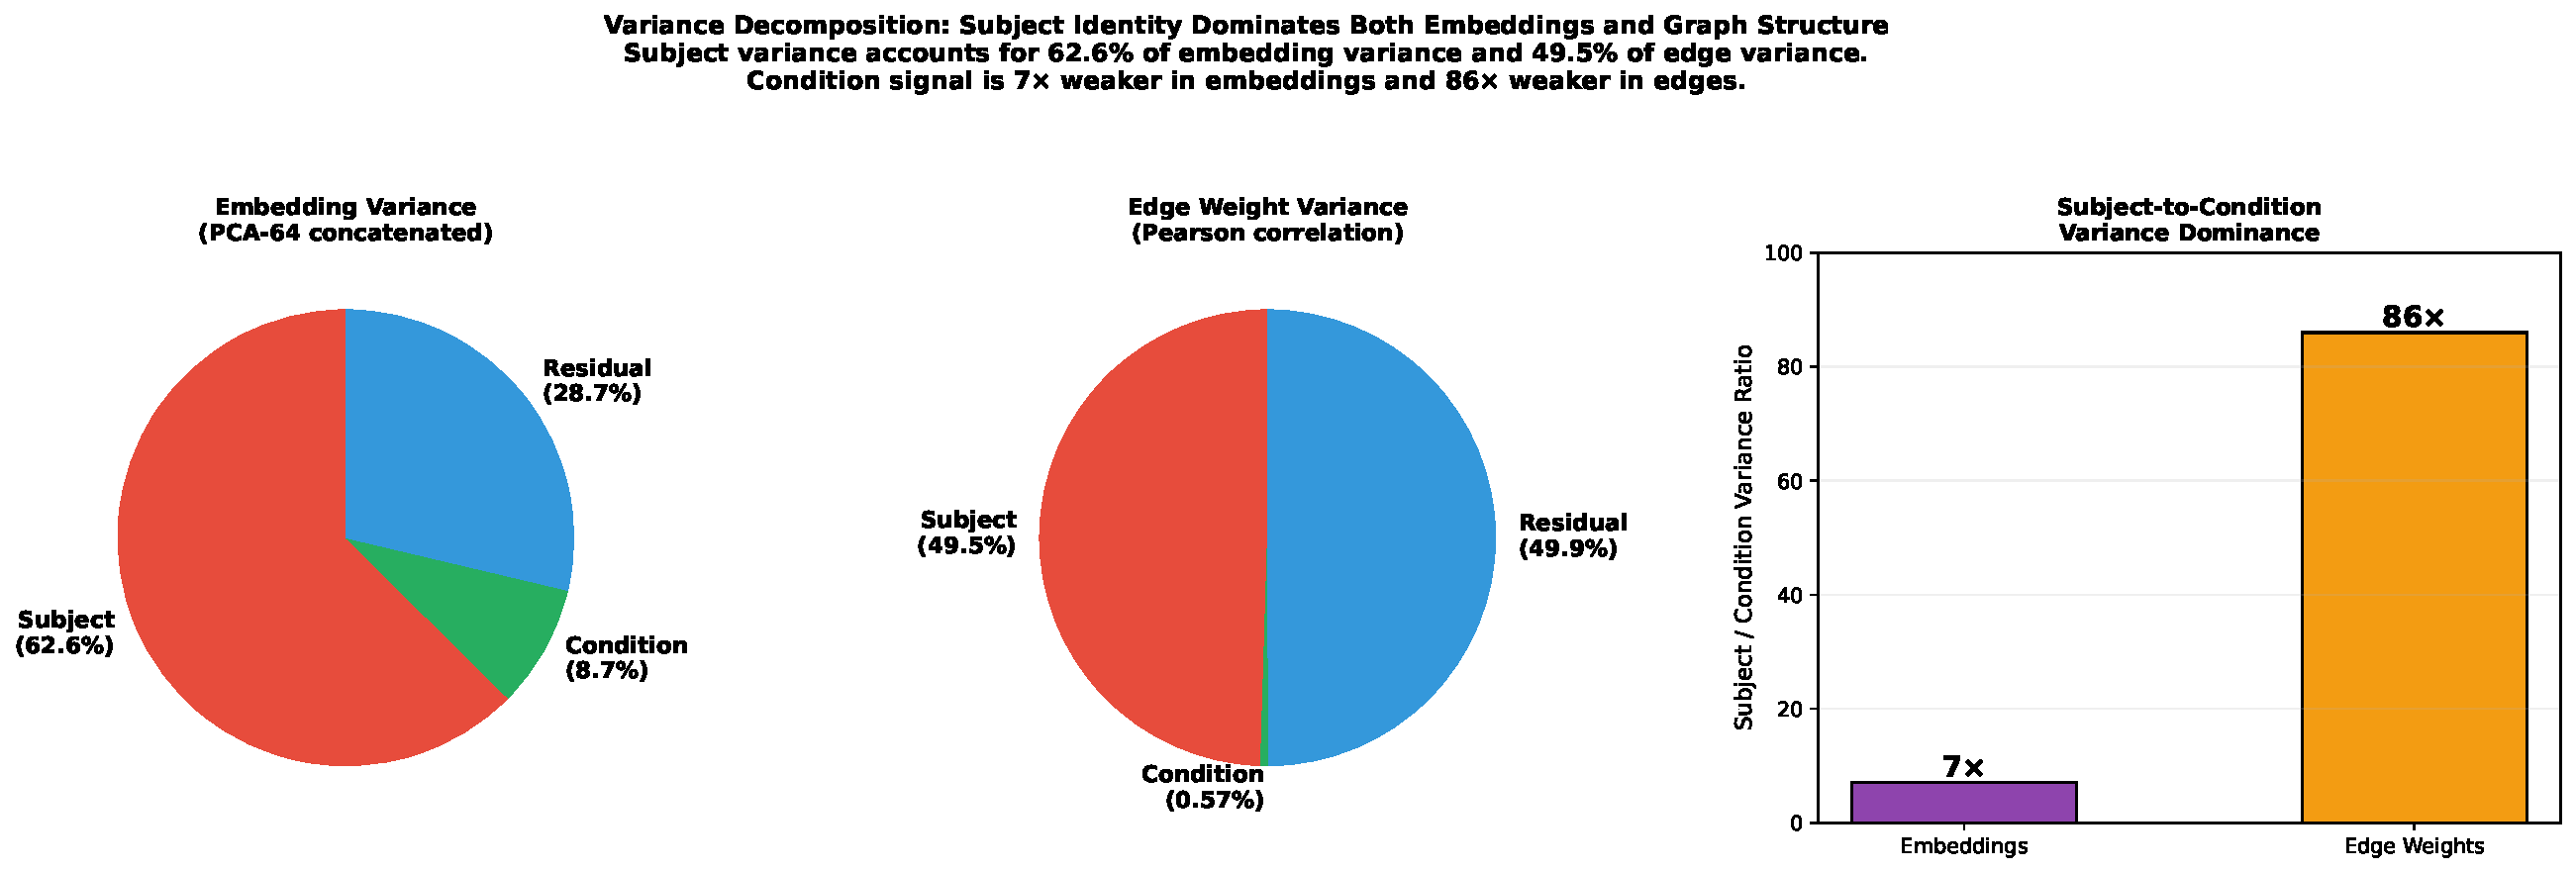
\includegraphics[width=\textwidth]{pictures/chGraphNeuralNetworks/exp01_variance_decomposition.pdf}
    \caption{Descriptive variance decomposition of the archived embedding and edge-weight spaces. Left: embedding partition (subject $62.6\%$, condition $8.7\%$, residual $28.7\%$). Center: edge-weight partition (subject $49.5\%$, condition $0.57\%$). Right: subject-to-condition ratios. These values depend on the earlier global-PCA graph construction.}
    \label{fig:exp01_variance}
\end{figure}

Subject identity accounts for $62.6\%$ of total embedding variance, emotional condition accounts for $8.7\%$, and within-subject residual variability accounts for $28.7\%$, a $7\times$ subject-to-condition ratio. At the graph-edge level, the dominance is more extreme: subject identity accounts for $49.5\%$ of edge-weight variance, condition accounts for only $0.57\%$ ($86\times$ ratio), and residual accounts for $49.9\%$. The classifier must detect an $8.7\%$ condition signal embedded in a representation dominated by subject-identity structure.

\subsection{Subject-Nuisance Suppression: Revealing the True Condition Signal}

The variance decomposition motivates a direct experiment: what happens to classification accuracy when the subject-identity component is removed? Six nuisance-suppression strategies were evaluated (Figure~\ref{fig:exp07_nuisance}).

\begin{figure}[H]
    \centering
    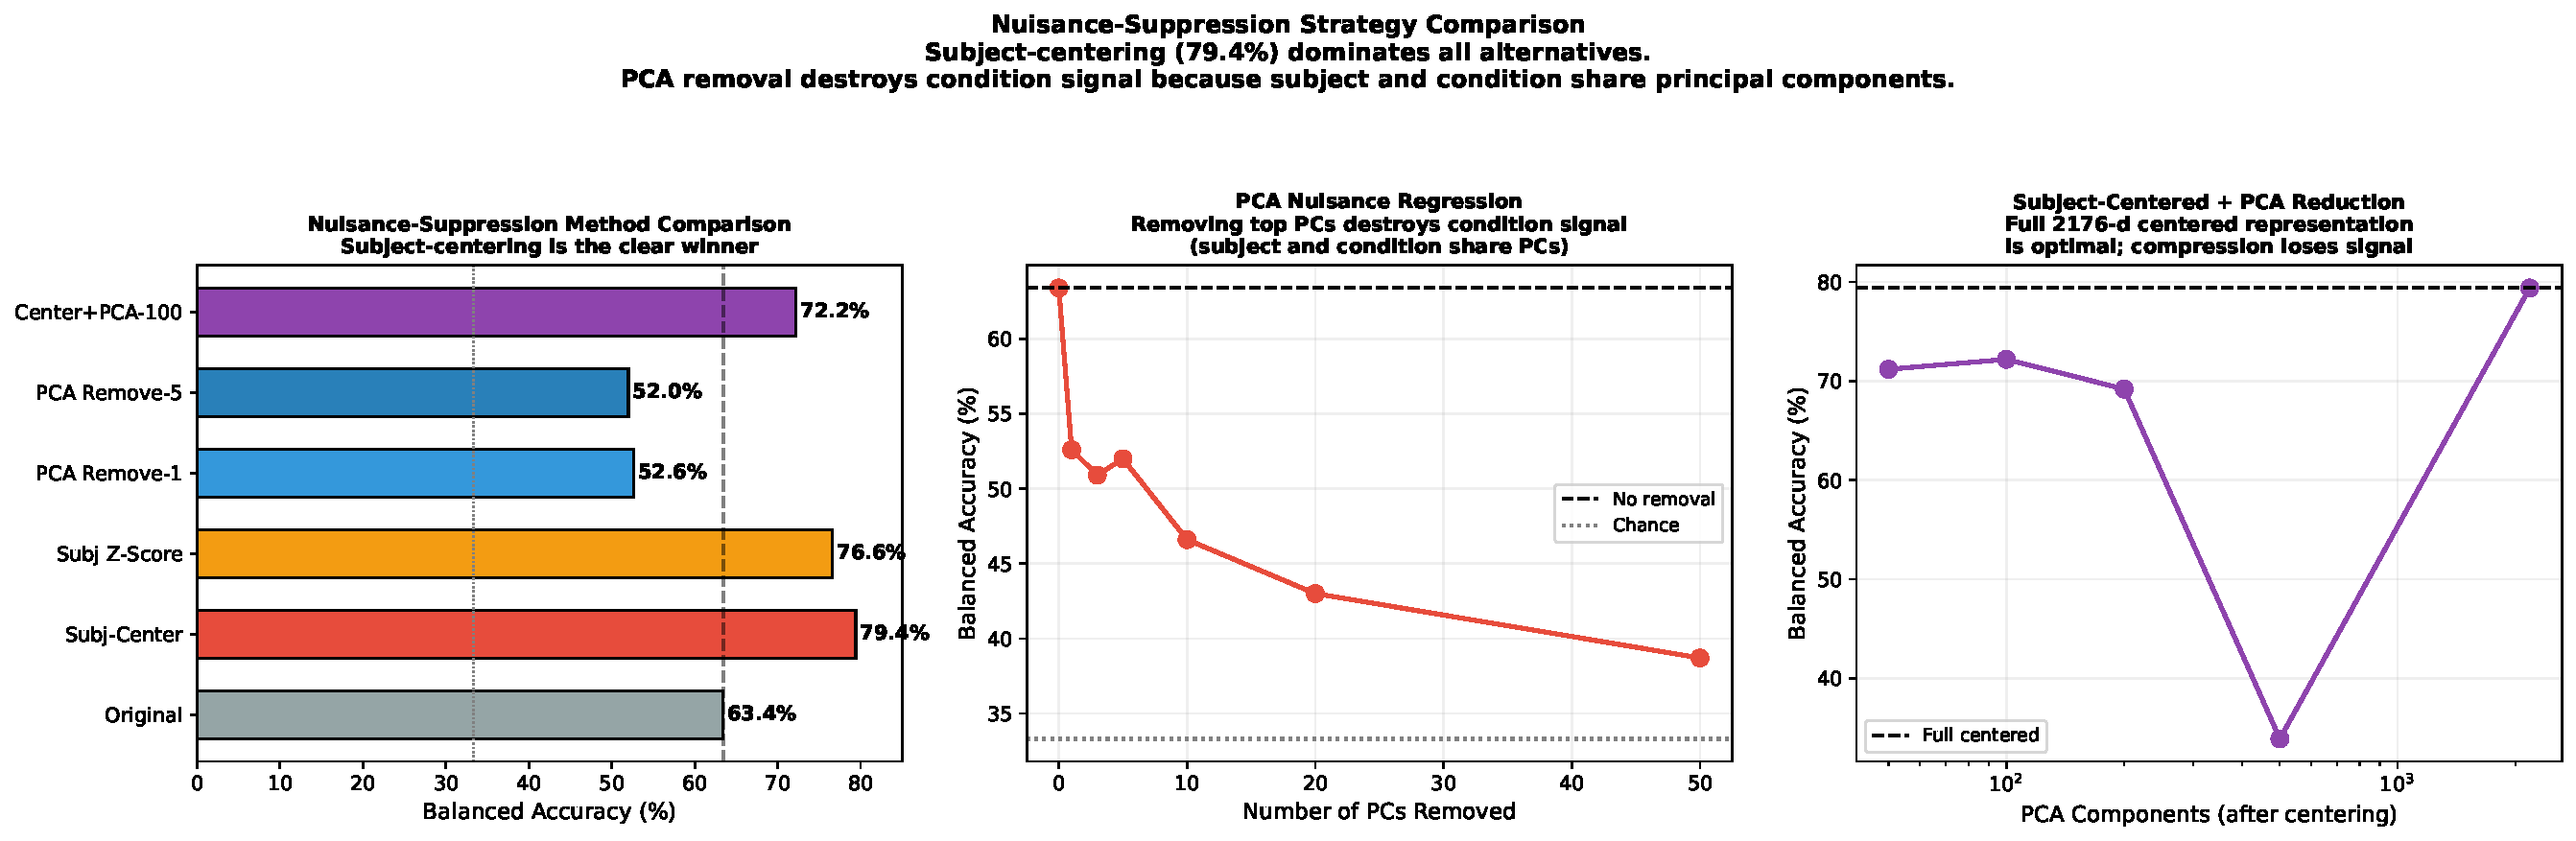
\includegraphics[width=\textwidth]{pictures/chGraphNeuralNetworks/exp07_nuisance_comparison.pdf}
    \caption{Archived normalization comparison. Per-subject centering uses all three observations from each held-out subject and is therefore a transductive panel analysis, not a single-observation deployment estimate. PCA-dependent values also use the earlier global-PCA representation.}
    \label{fig:exp07_nuisance}
\end{figure}

In the archived analysis, per-subject centering---subtracting each subject's mean embedding across all three conditions---produces $79.4\% \pm 7.4\%$ balanced accuracy, compared with $63.4\%$ without centering. Within-subject z-scoring produces $76.6\% \pm 5.9\%$. These values describe a repeated-measures panel setting in which all three observations for a held-out subject are available together; they do not estimate performance for a new subject represented by a single observation.

PCA nuisance regression (projecting out the top-$k$ components) reduces the archived accuracy as more components are removed. This is consistent with, but does not prove, overlap between directions associated with subject and condition variation. Because PCA was fitted globally and the directions are data-dependent, the experiment cannot establish a population-level geometric identity between the two sources of variation.

Subject-centering followed by PCA compression to $100$ dimensions produces $72.2\%$ in the archived run, below the full $2{,}176$-dimensional centered value. That difference may reflect information loss, regularization, or preprocessing choices; it does not by itself locate condition information across dimensions.

\subsubsection{Methodological Status of Subject-Centering}

The operational definition of per-subject centering is: given all $K$ observations from subject $s$ (here $K = 3$, one per condition), compute the subject mean $\bar{\mathbf{x}}_s = \frac{1}{K}\sum_{k=1}^K \mathbf{x}_{s,k}$ and subtract it from each observation: $\tilde{\mathbf{x}}_{s,k} = \mathbf{x}_{s,k} - \bar{\mathbf{x}}_s$. This is equivalent to the within-subject deviation from the subject's own baseline, the standard operation in repeated-measures experimental design.

Two methodological points require explicit statement. First, subject-centering uses all three held-out observations from each test subject. No labels and no training-subject observations enter that calculation, and no subject appears in both training and test folds. Nevertheless, the procedure uses feature data from the entire test-subject panel, so it is transductive with respect to the held-out subject and should be described as panel normalization rather than ordinary prospective prediction.

Second, per-subject centering is unavailable when a prospective subject contributes only one condition. The $79.4\%$ value is therefore neither a deployment estimate nor a theoretical ceiling; it is a descriptive result for the three-observation panel estimand. A prospective alternative would need to be specified, trained without access to held-out panels, and evaluated independently.

\subsection{Detection-Theoretic Analysis}

The archived analysis also summarized Negative--Neutral class geometry. Let $\mathbf{x} \in \mathbb{R}^d$ denote a representation vector with class-conditional means $\boldsymbol{\mu}_c$ and covariances $\boldsymbol{\Sigma}_c$. Four retained summaries describe different aspects of separation; none is an independent estimate of generalization performance.

\textbf{Sensitivity index (d$'$)} measures the standardized mean difference along each feature dimension: $d'_j = |\mu_{0,j} - \mu_{1,j}| / \sqrt{(\sigma_{0,j}^2 + \sigma_{1,j}^2)/2}$. The mean and maximum over dimensions characterize the average and peak per-feature discriminability.

\textbf{Bhattacharyya distance} summarizes overlap under a Gaussian approximation and can be used in bounds on Bayes error. Here it is computed with diagonal covariance matrices:
\begin{equation}
D_B = \frac{1}{8}(\boldsymbol{\mu}_0-\boldsymbol{\mu}_1)^\top
\boldsymbol{\Sigma}_{\mathrm{avg}}^{-1}(\boldsymbol{\mu}_0-\boldsymbol{\mu}_1)
+\frac{1}{2}\ln\!\left(
\frac{|\boldsymbol{\Sigma}_{\mathrm{avg}}|}
{|\boldsymbol{\Sigma}_0|^{1/2}|\boldsymbol{\Sigma}_1|^{1/2}}
\right).
\end{equation}

\textbf{Fisher Discriminant Ratio} measures the ratio of between-class to within-class scatter: FDR $= \text{tr}(\mathbf{S}_W^{-1}\mathbf{S}_B)$, with Tikhonov regularization for rank-deficient $\mathbf{S}_W$.

\textbf{Mahalanobis distance} is $d_M = \sqrt{(\boldsymbol{\mu}_0 - \boldsymbol{\mu}_1)^\top \boldsymbol{\Sigma}_{\text{pool}}^{-1} (\boldsymbol{\mu}_0 - \boldsymbol{\mu}_1)}$, measuring class separation in pooled-covariance-normalized space.

An earlier version also reported $\tfrac{1}{2}\sum_j\ln(1+d_j'^2)$ as a mutual-information lower bound. That expression is not a valid general lower bound for these correlated, multiclass features and can exceed the entropy of the three-class label. It is therefore omitted from the interpretation.

\begin{figure}[H]
    \centering
    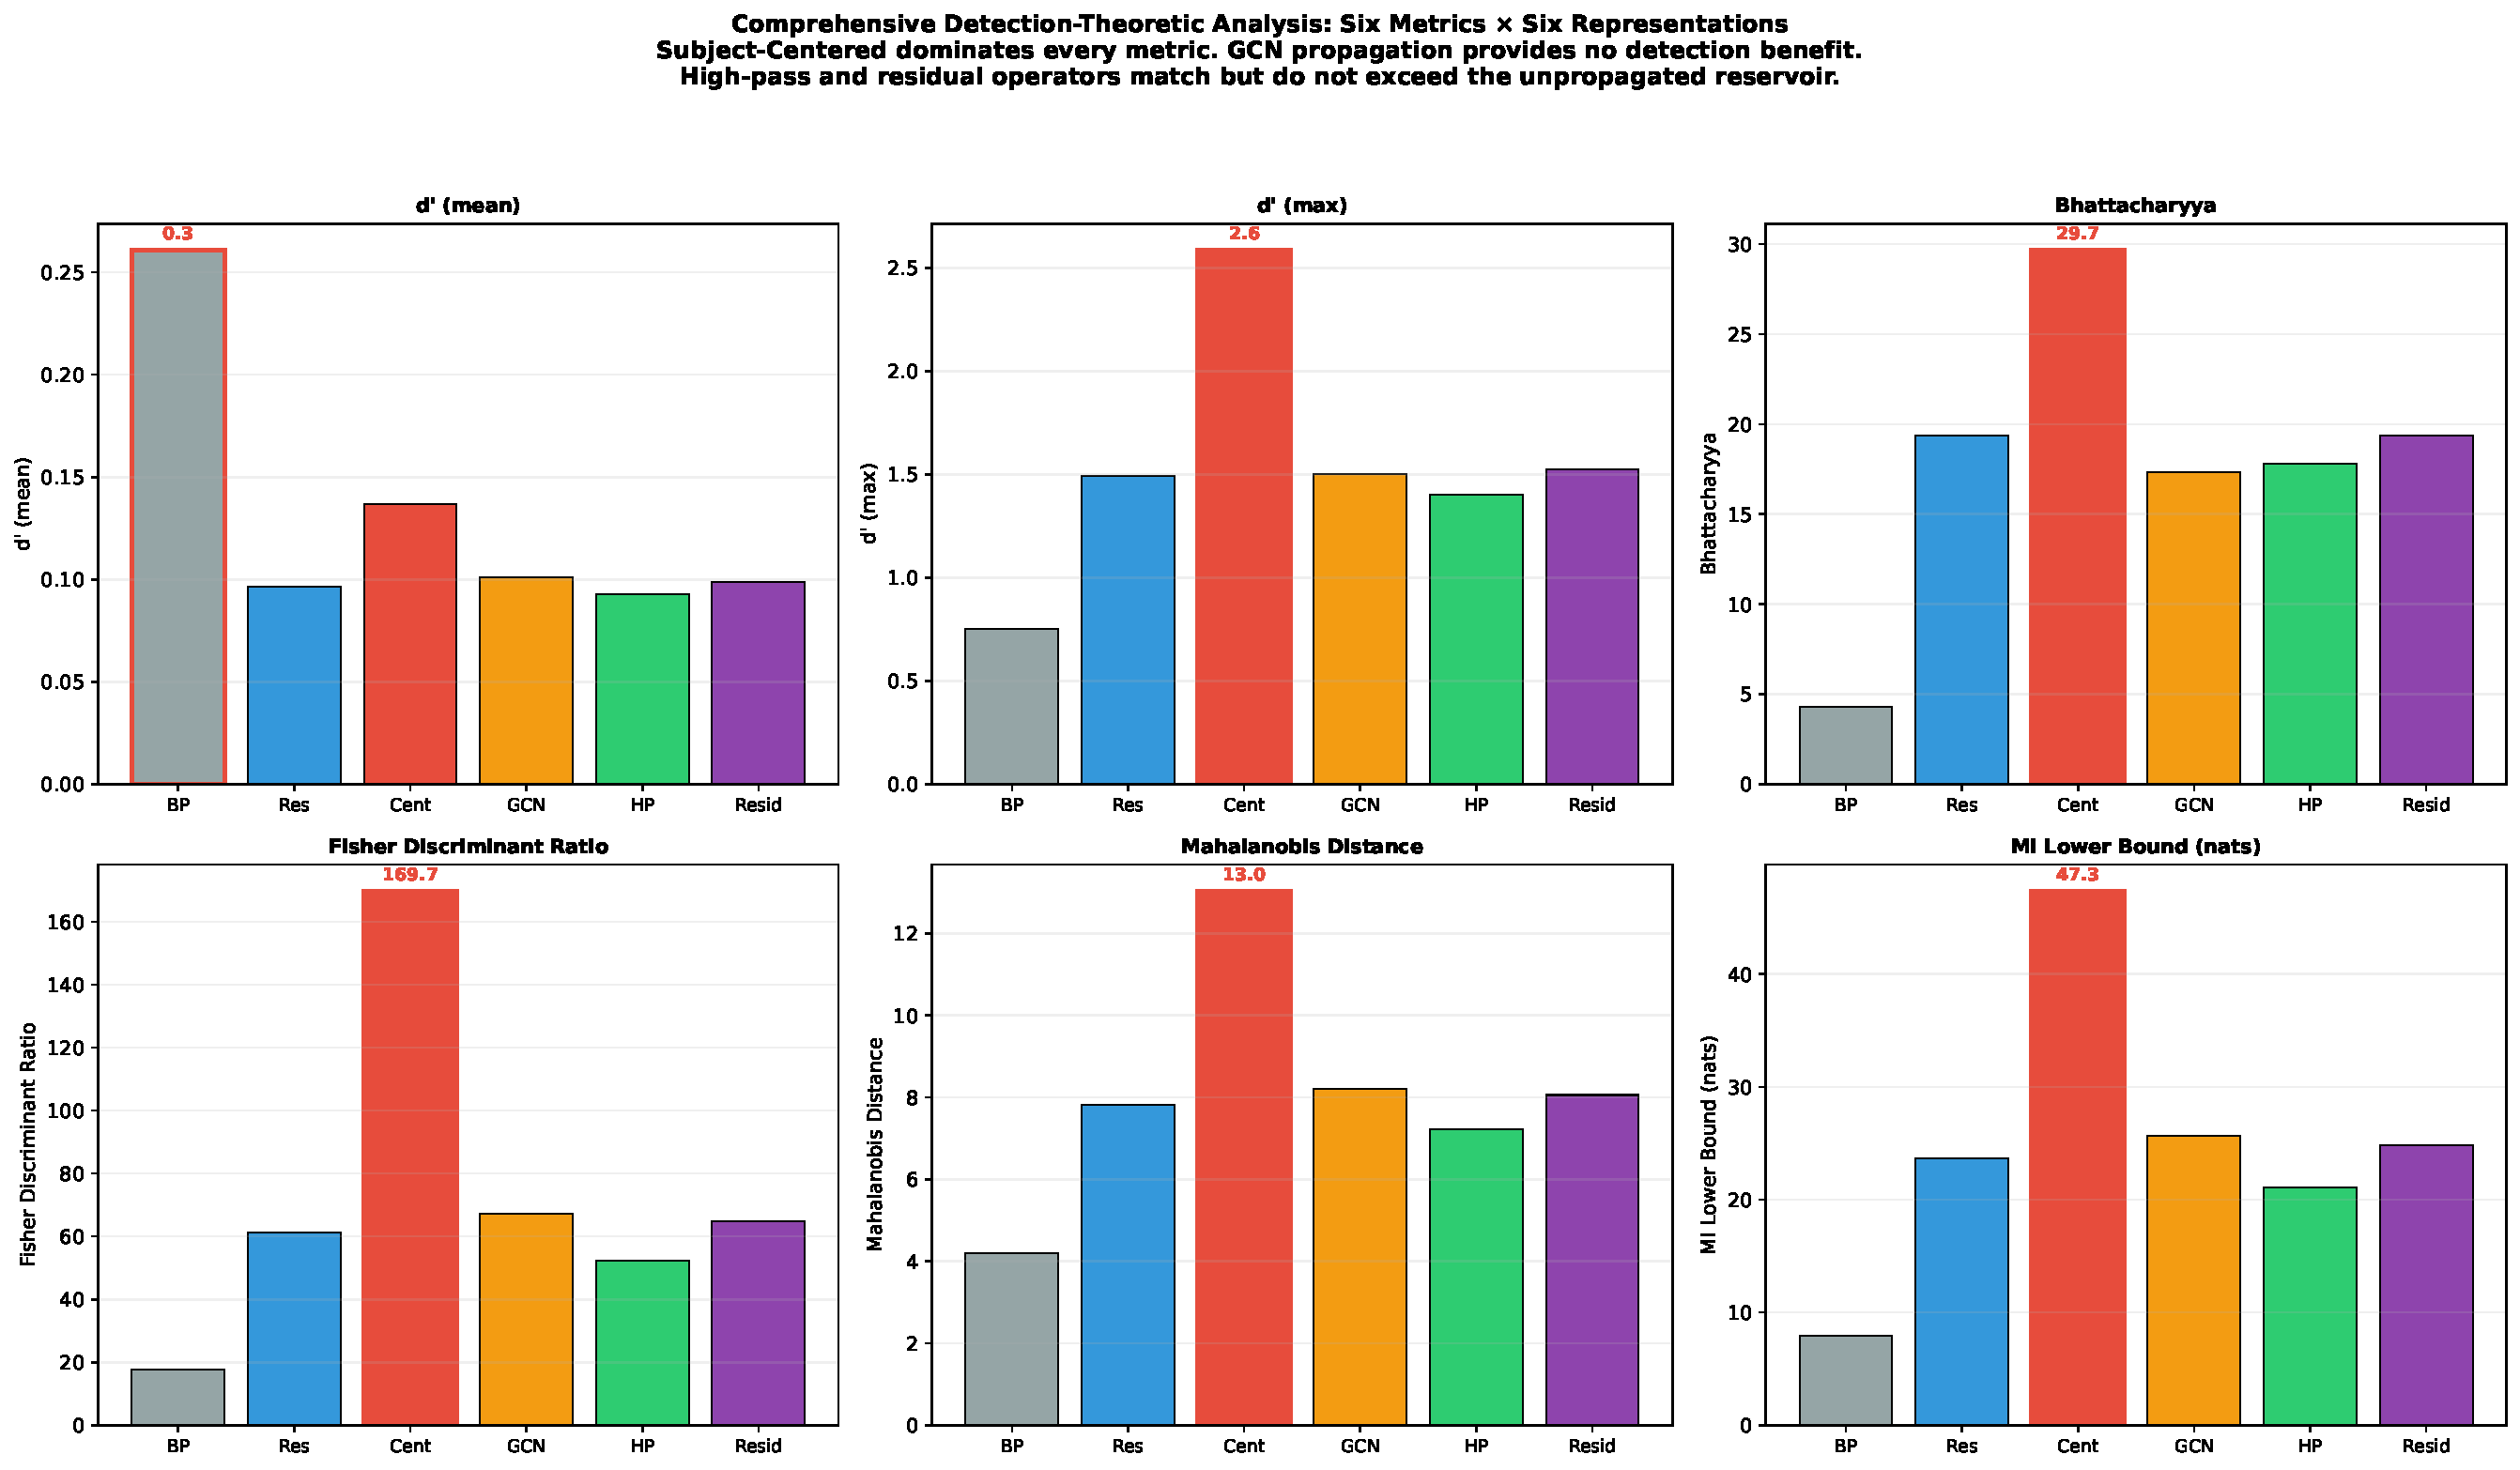
\includegraphics[width=\textwidth]{pictures/chGraphNeuralNetworks/exp08_detection_metrics.pdf}
    \caption{Archived class-geometry summaries for Negative versus Neutral. The mutual-information panel in the archived figure used an invalid estimator and is not interpreted. PCA-dependent quantities are descriptive because the earlier pipeline fitted PCA globally.}
    \label{fig:exp08_detection}
\end{figure}

In the archived representation, the reservoir features have maximum sensitivity index $d'_{\max}=1.49$, diagonal-approximation Bhattacharyya distance $19.4$, Fisher ratio $61.1$, and regularized Mahalanobis distance $7.82$. The corresponding panel-centered values are larger. These in-sample summaries depend on global preprocessing and covariance regularization, so they are descriptive comparisons rather than a count of information units.

\subsubsection{Spectral Interpretation of the Archived Propagation Sweep}

Let $\hat{\mathbf{A}}$ denote a symmetric normalized adjacency with eigendecomposition $\hat{\mathbf{A}}=\mathbf{U}\boldsymbol{\Lambda}\mathbf{U}^{\top}$. Linear propagation gives $\mathbf{H}^{(K)}=\hat{\mathbf{A}}^K\mathbf{H}^{(0)}=\mathbf{U}\boldsymbol{\Lambda}^K\mathbf{U}^{\top}\mathbf{H}^{(0)}$. Thus a graph-spectral component associated with eigenvalue $\mu_i$ is multiplied by $\mu_i^K$.

This identity explains spectral attenuation, but attenuation alone does not prove that standardized class detectability must decrease: propagation can change class means and within-class covariance together. The archived sweep shows decreasing accuracy for the tested operators and graphs, which is consistent with useful contrast being attenuated in those runs. It does not establish a general propagation--detectability theorem.

Per-subject centering operates across a subject's observations, whereas graph propagation operates across channel nodes. The subject mean is therefore not the channel graph's zero-frequency component, and the two operations should not be assigned complementary graph-frequency roles. Their empirical effects are reported separately.


\section{Graph Propagation Regime Characterization}
\label{sec:ch5_regime}

In the archived implementation, message-passing propagation does not improve the displayed classification result. The propagation sweep describes how that implementation changes as depth and density vary; it does not locate a universal regime boundary.

\subsection{Propagation Operating Characteristic}

Figure~\ref{fig:exp03_poc} presents accuracy, inter-channel variance, and pairwise cosine similarity across propagation depths from $0$ to $5$. Graph densities are $5\%$, $10\%$, $15\%$, $20\%$, $30\%$, and $50\%$, producing $36$ operating points.

\begin{figure}[H]
    \centering
    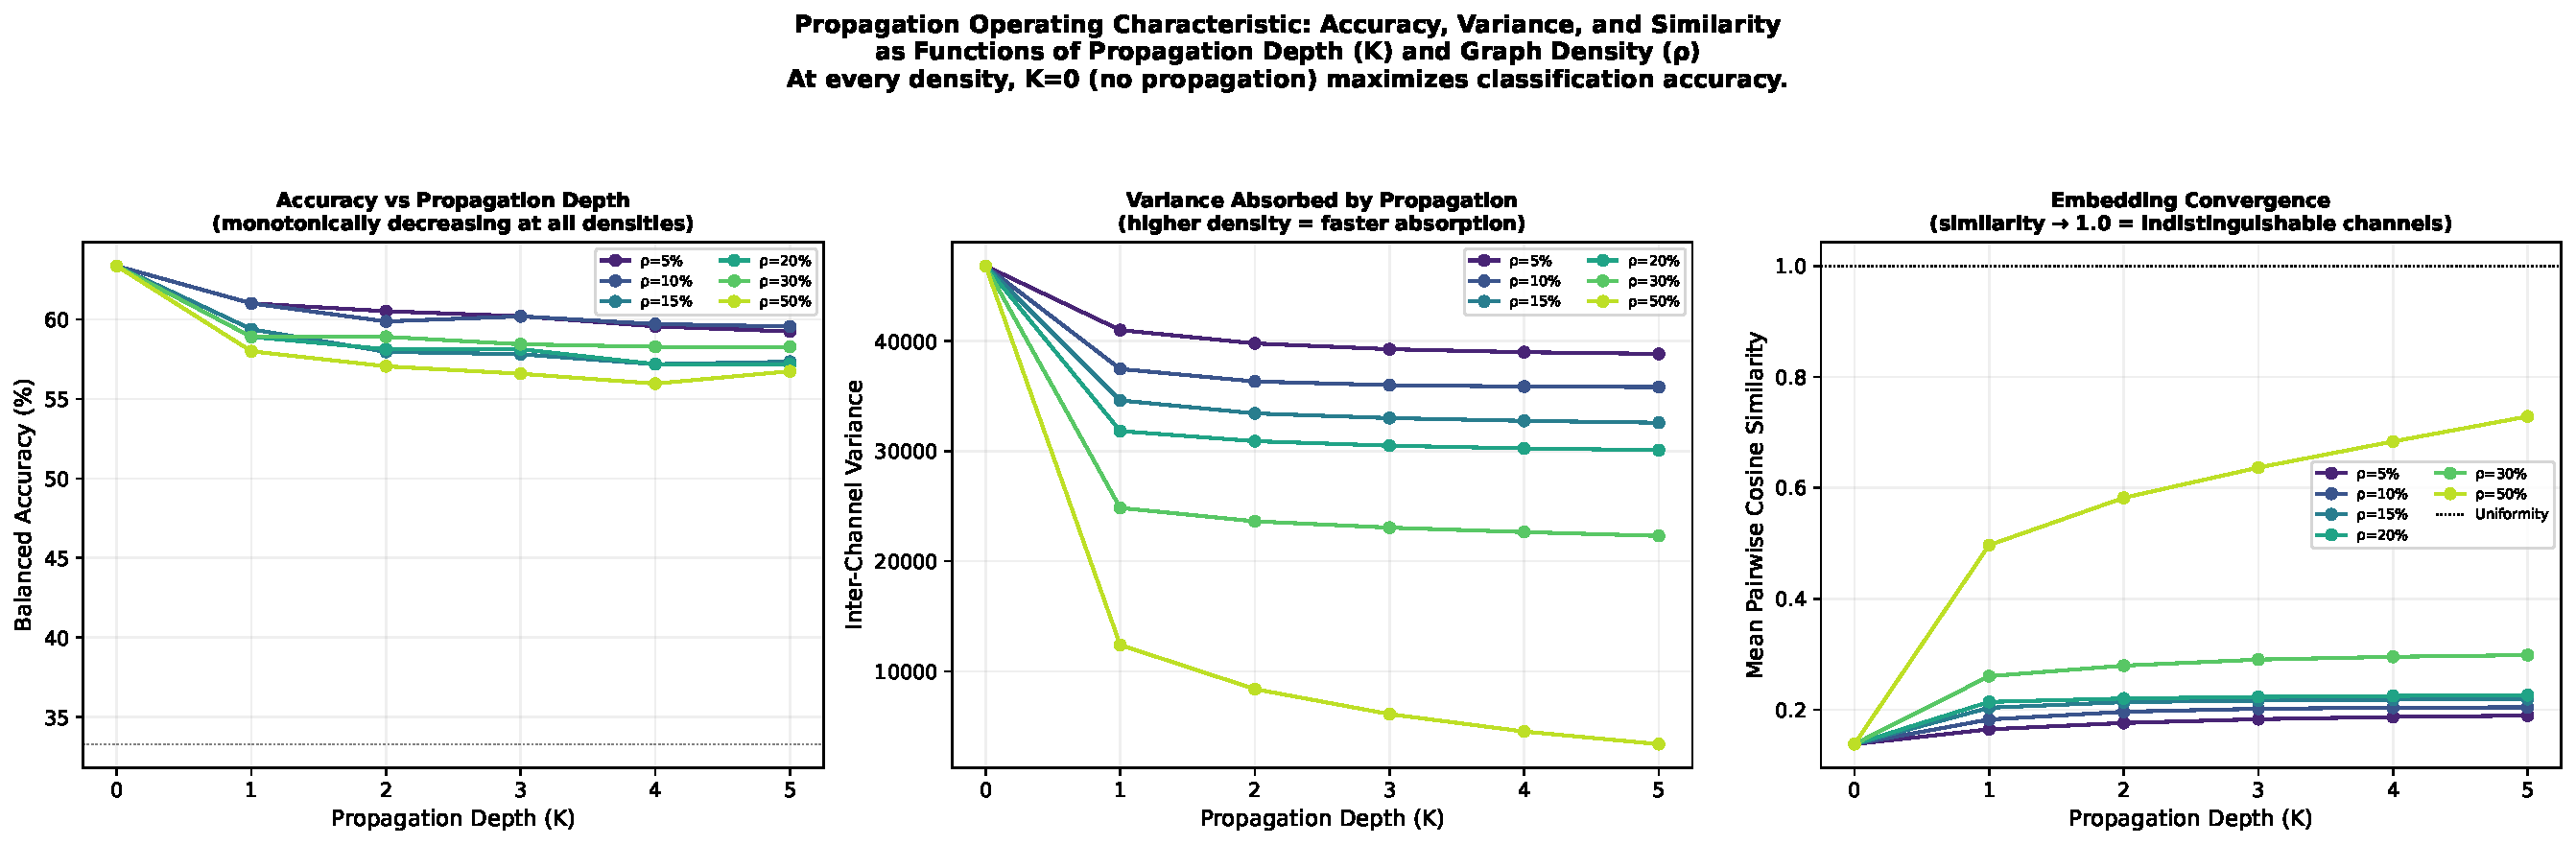
\includegraphics[width=\textwidth]{pictures/chGraphNeuralNetworks/exp03_propagation_operating_characteristic.pdf}
    \caption{Archived propagation sweep ($6$ densities $\times$ $6$ depths). Within these runs, the displayed accuracy decreases with depth, inter-channel variance decreases, and cosine similarity increases. PCA was fitted globally, so values are descriptive legacy estimates.}
    \label{fig:exp03_poc}
\end{figure}

Three observations emerge. First, classification accuracy is \emph{monotonically decreasing} in $K$ at every density tested. The maximum accuracy is always at $K = 0$ (no propagation). At $\rho = 20\%$, two layers reduce accuracy from $63.4\%$ to $58.1\%$; at $\rho = 50\%$, from $63.4\%$ to $57.0\%$.

Second, inter-channel variance decreases monotonically with $K$, and the rate of decrease accelerates with density. At $\rho = 20\%$ and $K = 2$, variance drops by $34\%$; at $\rho = 50\%$ and $K = 4$, by $90\%$. This quantifies the smoothing mechanism: each propagation layer absorbs inter-channel discriminative contrast.

Third, pairwise cosine similarity increases monotonically with $K$, from $0.138$ at $K = 0$ to $0.684$ at $\rho = 50\%$, $K = 4$, indicating that channel embeddings converge toward a common profile. The channel identity that carries the classification signal is progressively erased.

\subsection{Graph Construction Sweep}

Figure~\ref{fig:exp04_sweep} compares the archived estimate under three adjacency constructions: thresholded PCA-coordinate similarity, an assumed spatial-distance graph, and a degree-matched random graph. All three displayed $K=2$ values are lower than the $K=0$ comparison. The channel montage used for the spatial graph was not verified.

All three tested constructions produce lower archived accuracy than the non-propagated comparison. This shows that none improved that implementation; it does not demonstrate that graph size or density is the cause. In particular, the Pearson graph is a feature-similarity construction and, given the PCA-basis limitation described above, should not be called a physiological functional-connectivity graph.

\begin{figure}[H]
    \centering
    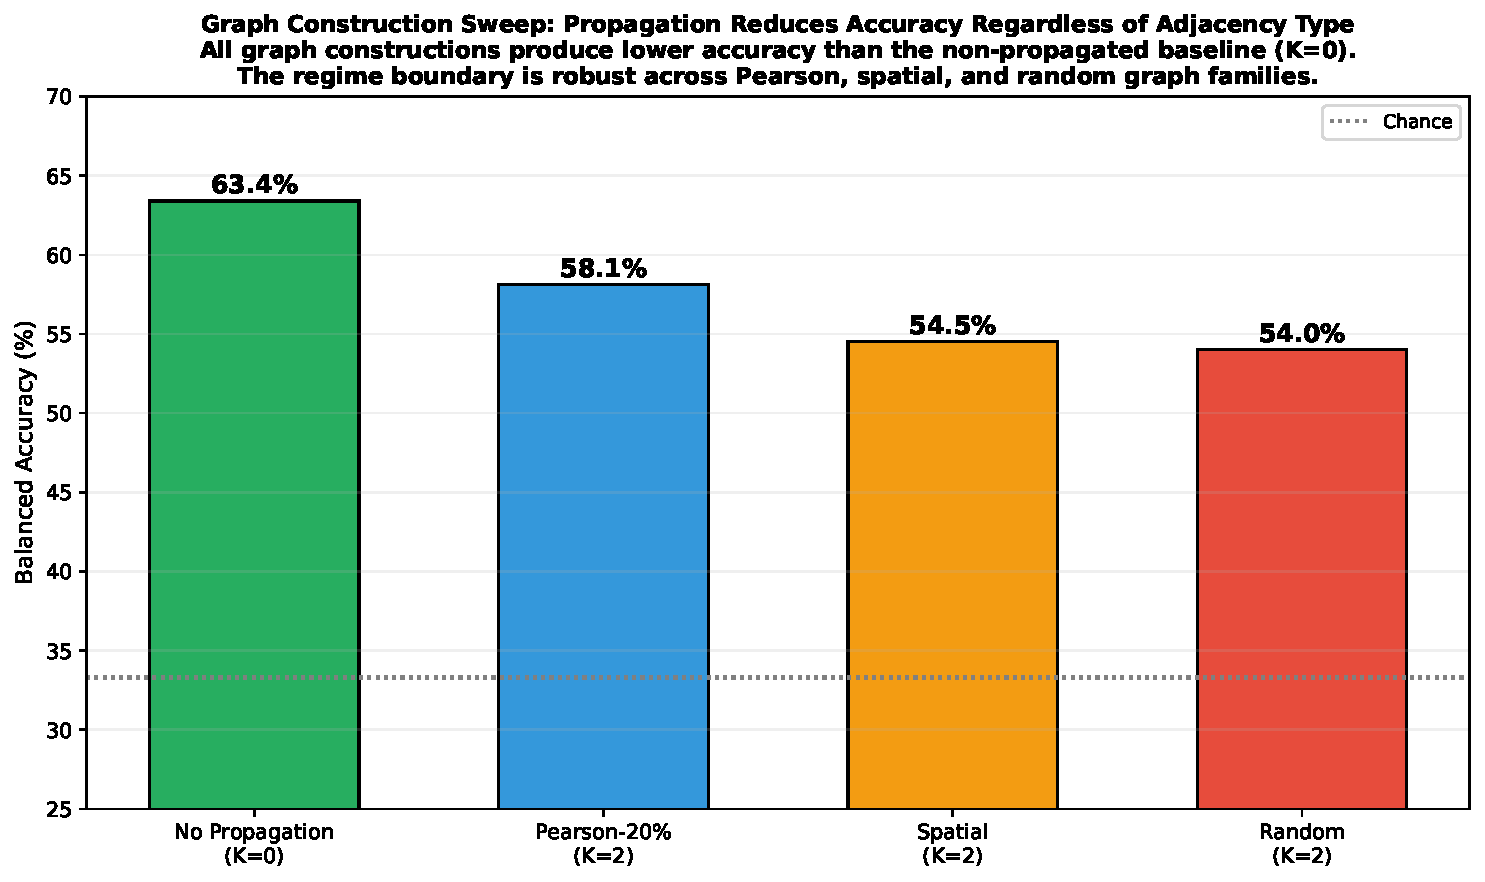
\includegraphics[width=\textwidth]{pictures/chGraphNeuralNetworks/exp04_graph_construction_sweep.pdf}
    \caption{Archived graph-construction sweep. The tested Pearson-similarity, assumed-spatial, and random constructions produce lower displayed accuracy at $K=2$ than the $K=0$ comparison. The montage used for the spatial construction was not verified.}
    \label{fig:exp04_sweep}
\end{figure}

\subsection{Heterophily-Aware and Contrast-Preserving Graph Operators}

The observation that standard smoothing-based message-passing reduces accuracy raises a natural question: do contrast-preserving graph operators recover or exceed the non-propagated baseline? The smoothing hypothesis predicts that operators designed to preserve or amplify inter-channel differences should avoid the variance-absorption mechanism observed in standard GCN propagation. Four contrast-preserving operator families were evaluated (Figure~\ref{fig:exp06_operators}).

\begin{figure}[H]
    \centering
    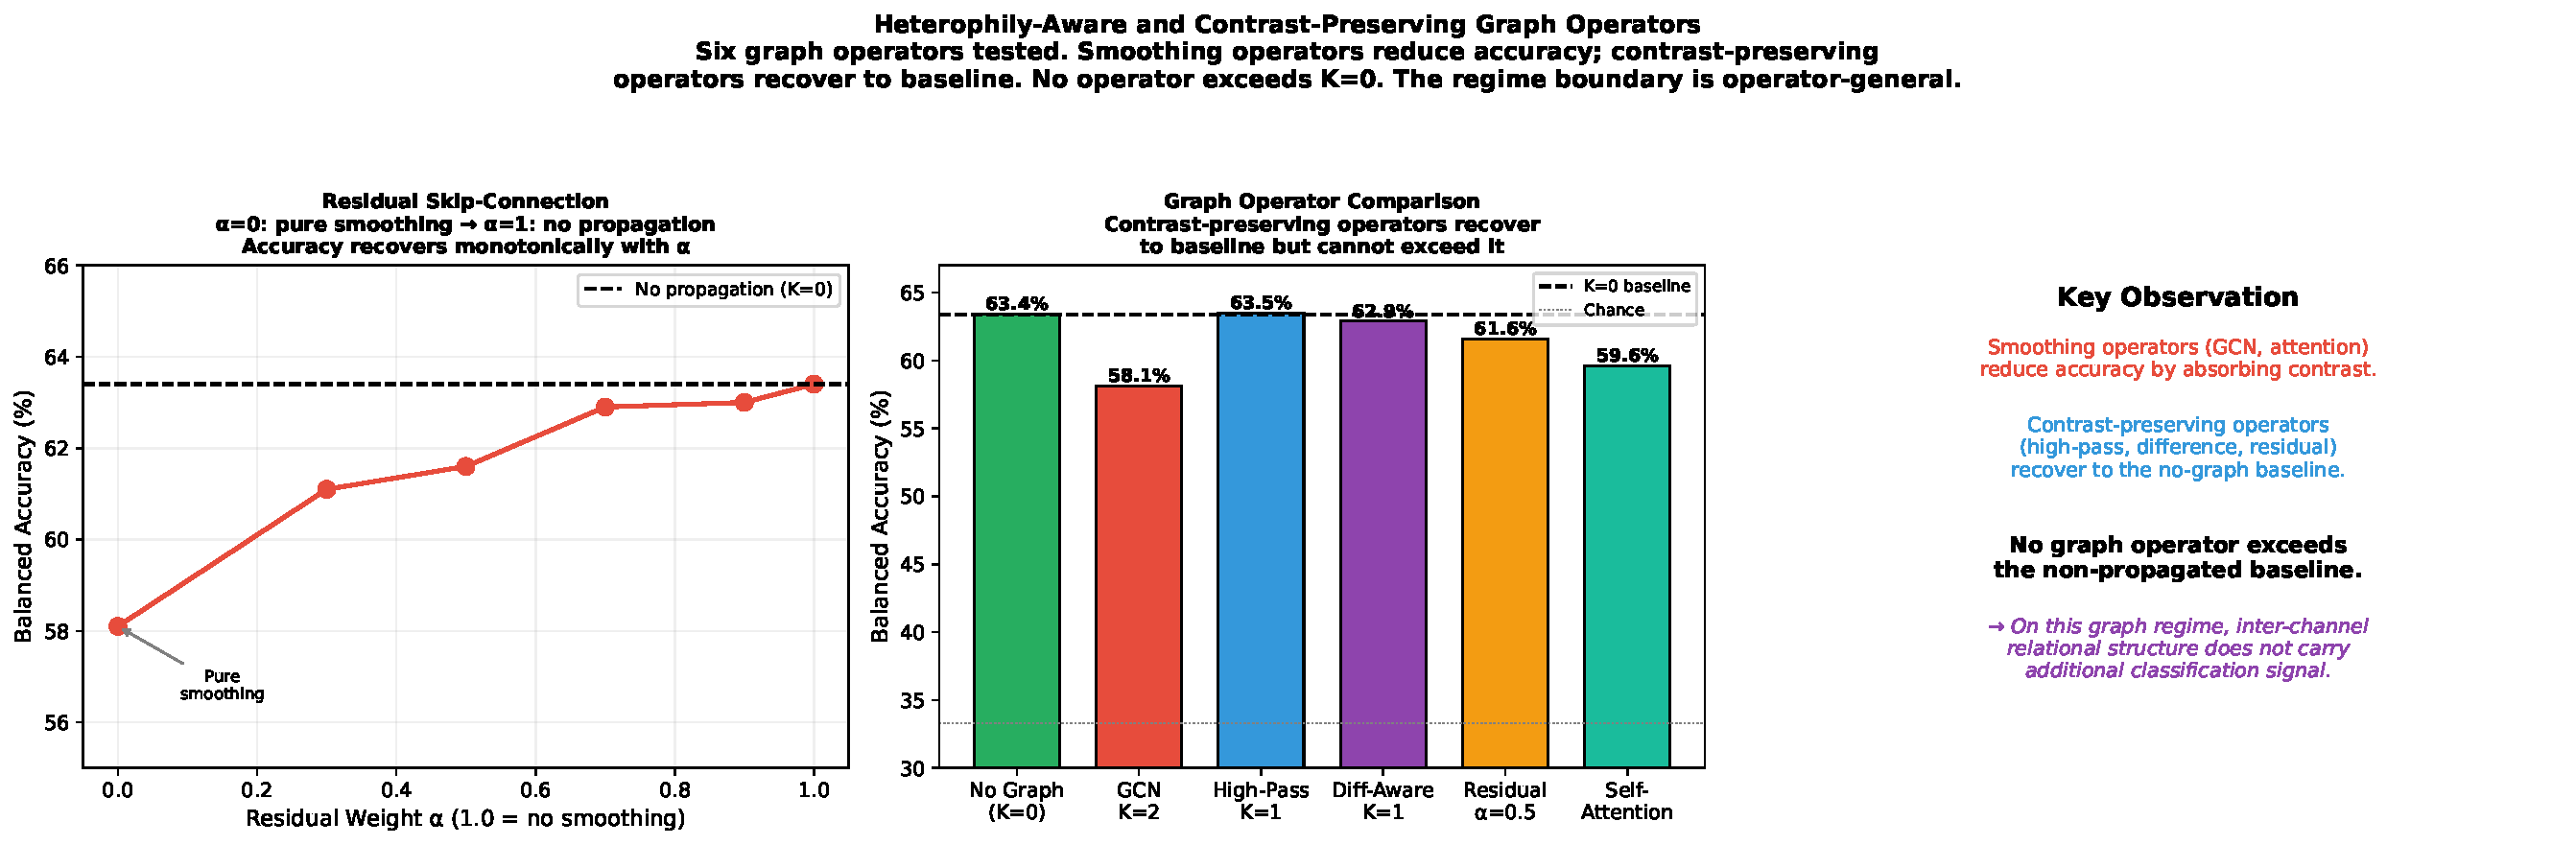
\includegraphics[width=\textwidth]{pictures/chGraphNeuralNetworks/exp06_heterophily_operators.pdf}
    \caption{Archived graph-operator analysis. Left: residual skip-connection sweep, from pure smoothing ($\alpha=0$) to no propagation ($\alpha=1$). Center: the tested contrast-preserving operators approach the $K=0$ comparison. Right: summary of the measured values.}
    \label{fig:exp06_operators}
\end{figure}

\textbf{Residual skip-connection} ($\mathbf{H}^{(k+1)} = \alpha \mathbf{H}^{(0)} + (1-\alpha)\hat{\mathbf{A}}\mathbf{H}^{(k)}$): the archived point estimate increases with $\alpha$, from $58.1\%$ at $\alpha = 0$ to $63.4\%$ at $\alpha = 1$. The largest displayed value is therefore the identity, or no-propagation, endpoint; no nested selection test establishes a generally optimal setting.

\textbf{High-pass graph filter} ($\mathbf{H}^{(k+1)} = (2\mathbf{I} - \hat{\mathbf{A}})\mathbf{H}^{(k)}$): amplifies differences between neighboring channels rather than smoothing them. Achieves $63.5\%$ at $K = 1$, matching the baseline within noise.

\textbf{Signed-difference aggregation} (aggregate $|\mathbf{h}_i - \mathbf{h}_j|$ across neighbors): achieves $62.9\%$ at $K = 1$, again matching the baseline.

\textbf{Channel self-attention} (softmax attention across all channels, no graph constraint): achieves $59.6\%$, below the baseline, indicating that even learned attention weights absorb discriminative contrast on this small array.

In the archived comparisons, smoothing operators reduce accuracy and the contrast-preserving variants approach, but do not clearly exceed, the non-propagated result. Seven named operator families were considered (GCN, GIN, EdgeConv, high-pass, residual, difference-aware, and self-attention). This is evidence about the tested configurations only; it does not establish that all inter-channel relational structure is uninformative.


\section{Exploratory Graph-Topological Associations}
\label{sec:ch5_interpretability}

The graph summaries were screened against multiple clinical variables, node metrics, edges, and interaction terms. These analyses were not prespecified as a single confirmatory family. Unless an adjustment is stated, the $p$ values below are nominal; with many comparisons, some $p<0.05$ results are expected under the null. The strongest nominal SUD comparison does not reach $p<0.05$ in its label-permutation check. Accordingly, this section reports exploratory cohort associations and makes no phenotype or biomarker claim.

\subsection{Graph-Level Associations}

GAD has the only nominal graph-level association in this screen: participants with GAD ($n=60$) have greater degree heterogeneity in the archived graph ($d=+0.34$, nominal $p=0.032$). This result is uncorrected and does not establish a population association.

\subsection{Channel-Level Clinical Comparisons}

The uncorrected channel-level screen contains nominal $p<0.05$ comparisons for each clinical variable (Figure~\ref{fig:channel_biomarkers}). Counts of nominal results cannot be interpreted without the size and dependence structure of the tested family. Examples include Ch14 clustering for MDD ($d=-0.45$, nominal $p=0.003$), Ch3 clustering for PTSD ($d=+0.36$, nominal $p=0.011$), and several channel-strength comparisons for SUD. Because the channels are unlabeled, the PCA bases in the archived graph are not commensurate, and family-wise inference was not established, these observations do not support anatomical or connectivity interpretations.

\begin{figure}[H]
    \centering
    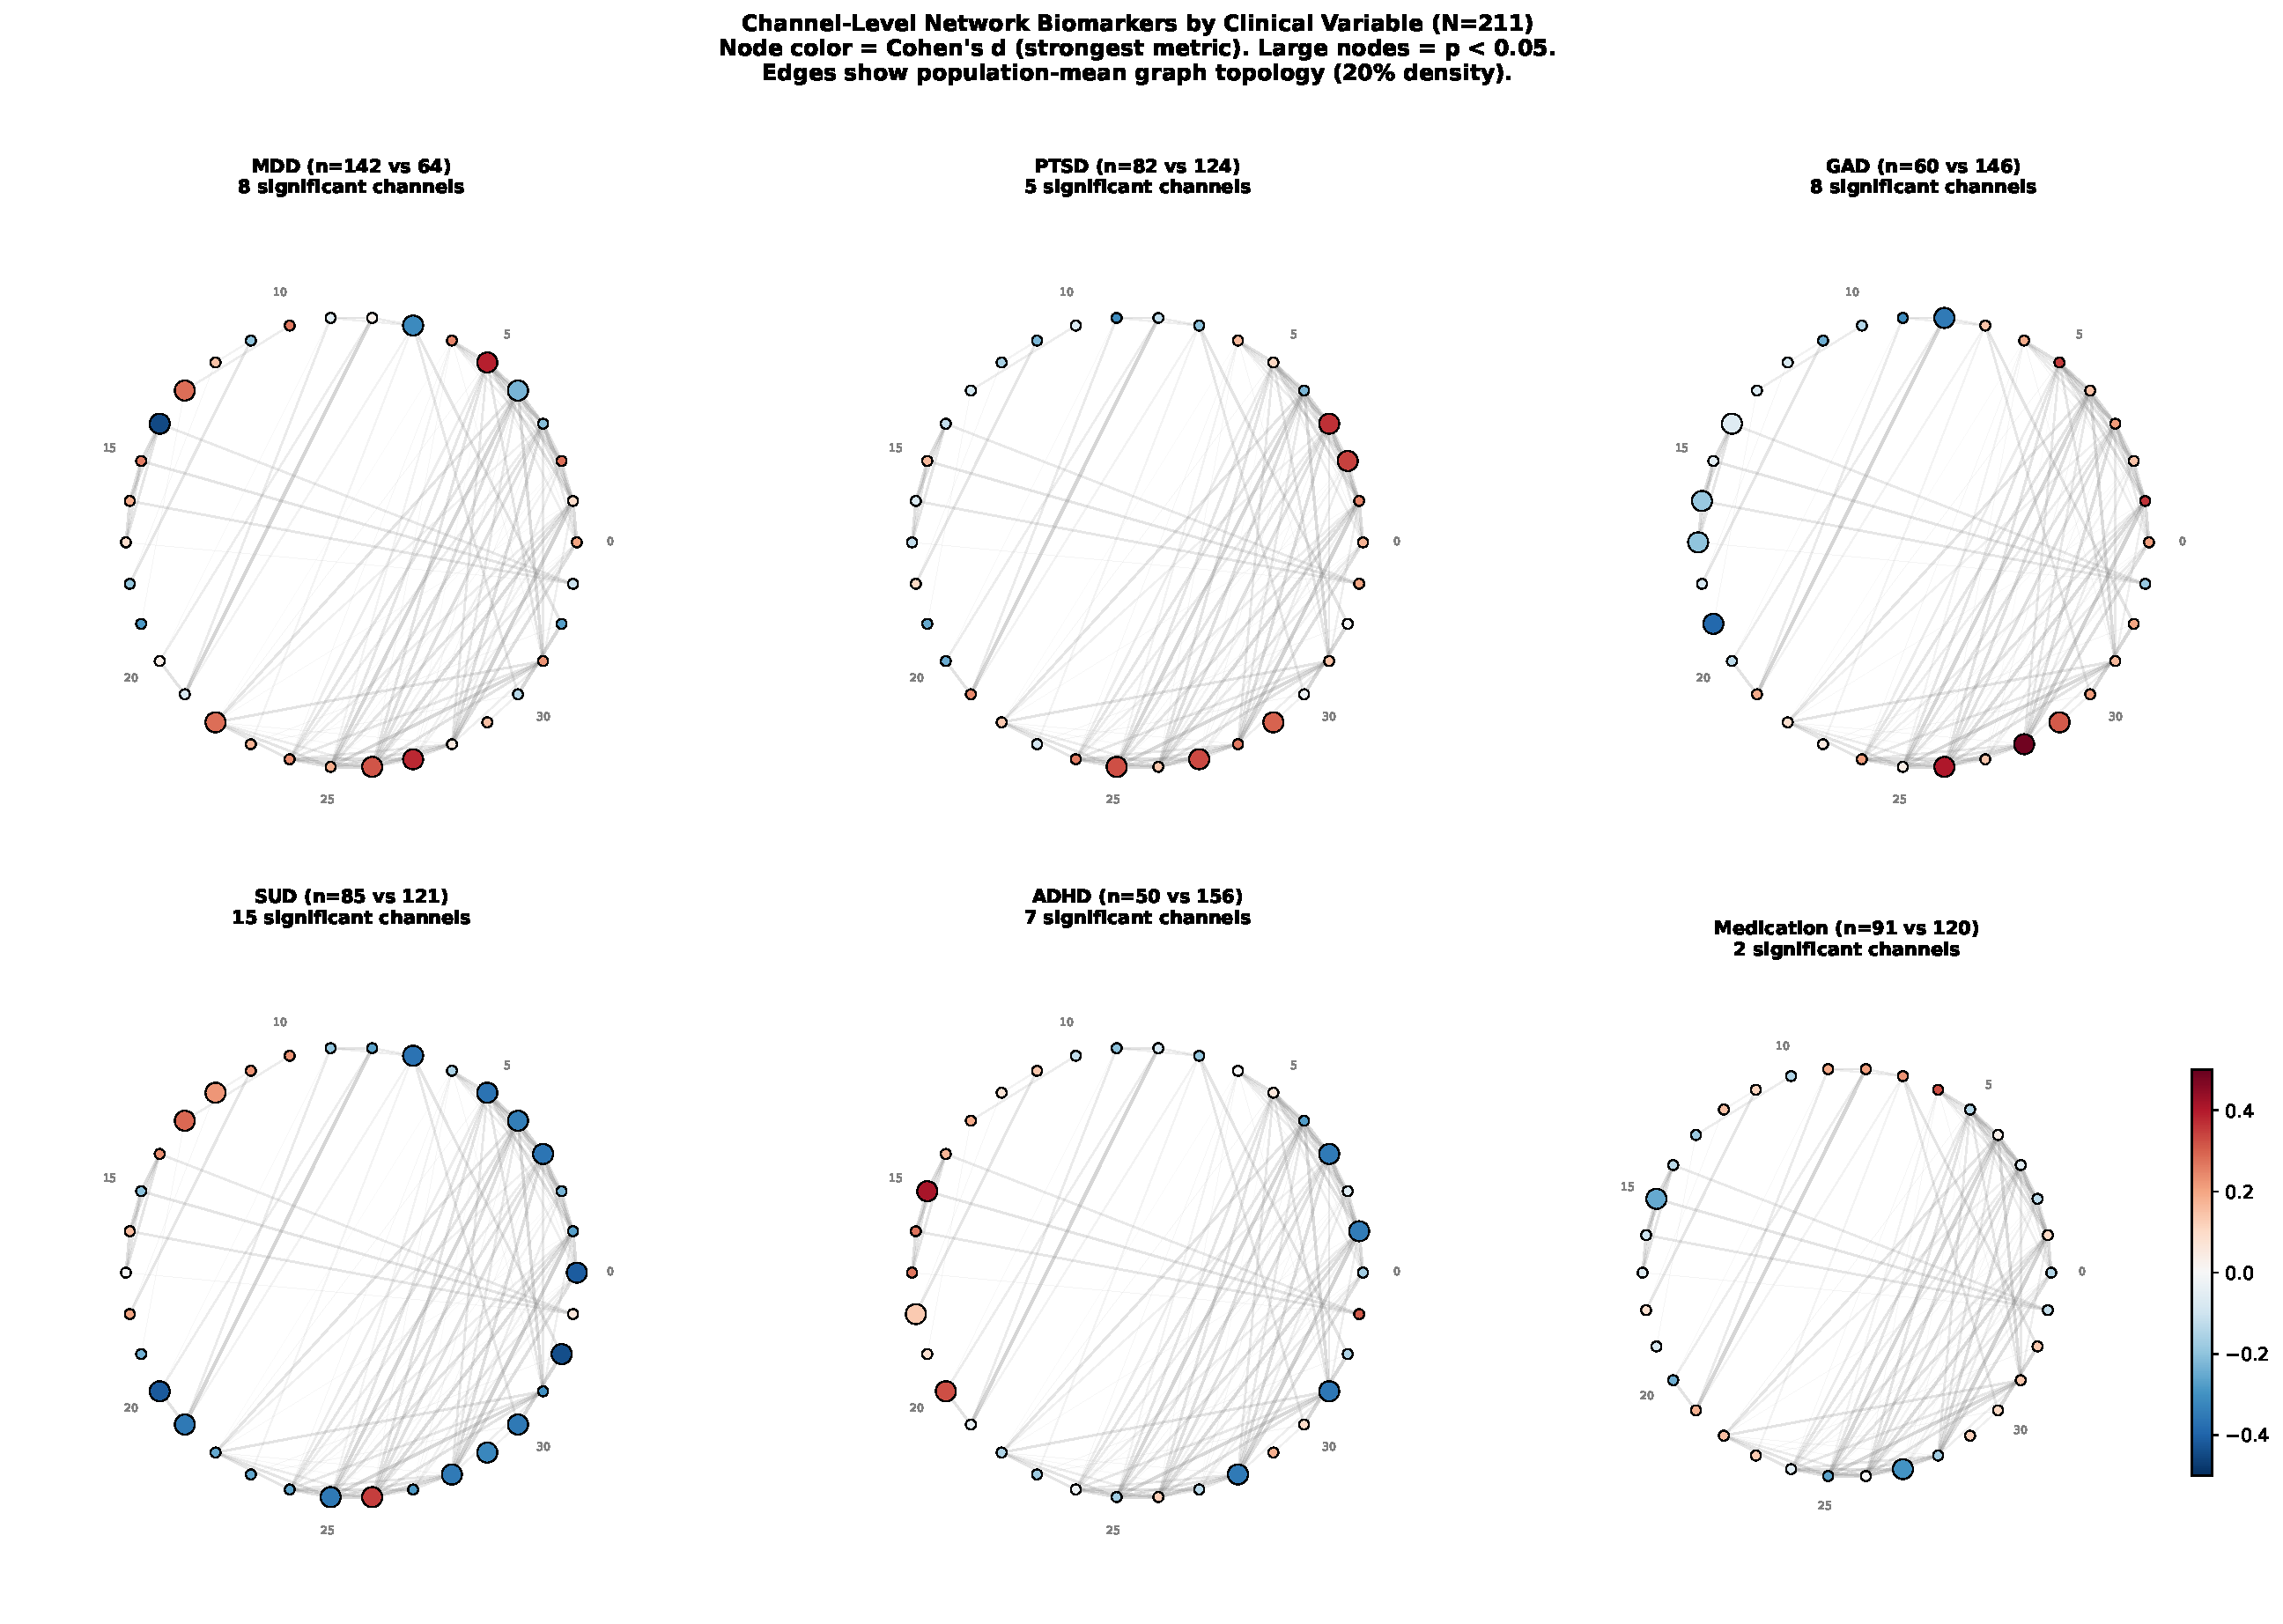
\includegraphics[width=\textwidth]{pictures/chGraphNeuralNetworks/fig_channel_biomarkers_211.pdf}
    \caption{Exploratory channel-level graph comparisons ($N=211$). Node color shows the largest displayed Cohen's $d$ and larger nodes mark nominal $p<0.05$. Results are uncorrected and channels are unlabeled.}
    \label{fig:channel_biomarkers}
\end{figure}

\subsection{Substance Use Disorder Screen}
\label{ssec:ch5_sud}

The smallest nominal $p$ value in the archived clinical screen occurs in an SUD reactivity comparison (Figure~\ref{fig:sud_interactions}). Three reported comparisons are summarized below, without confirmatory interpretation.

\textbf{SUD $\times$ Strength reactivity (nominal $p=0.0004$).} The parametric summary reports $d=-0.52$, with mean changes of $+0.037$ for the non-SUD group and $-0.023$ for the SUD group. The separate permutation output reports $d=-0.34$. The archived materials do not document enough detail to reconcile these effect-size estimates, so neither is treated as a definitive estimate.

\textbf{SUD $\times$ Efficiency reactivity (nominal $p=0.003$, $d=+0.43$).} The displayed group means change in opposite directions. Because the test is part of an exploratory family and uses the archived graph, the difference is not assigned a mechanistic interpretation.

\textbf{SUD $\times$ Clustering reactivity (nominal $p=0.012$, $d=-0.35$).} The displayed group means again change in opposite directions; this is an uncorrected descriptive comparison.

The three directions appear visually coherent, but they were selected from a larger screen and do not establish a coherent disorder mechanism. Comorbidity, medication, and other confounding were not isolated, and the graph values cannot be interpreted as direct neural connectivity.

For the SUD strength comparison, $5{,}000$ label permutations yield an empirical $p=0.073$ (Figure~\ref{fig:exp05_permutation}). The test therefore does not reject the permutation null at $\alpha=0.05$. The nominal parametric result is retained only as a hypothesis for future, prespecified analysis.

\begin{figure}[H]
    \centering
    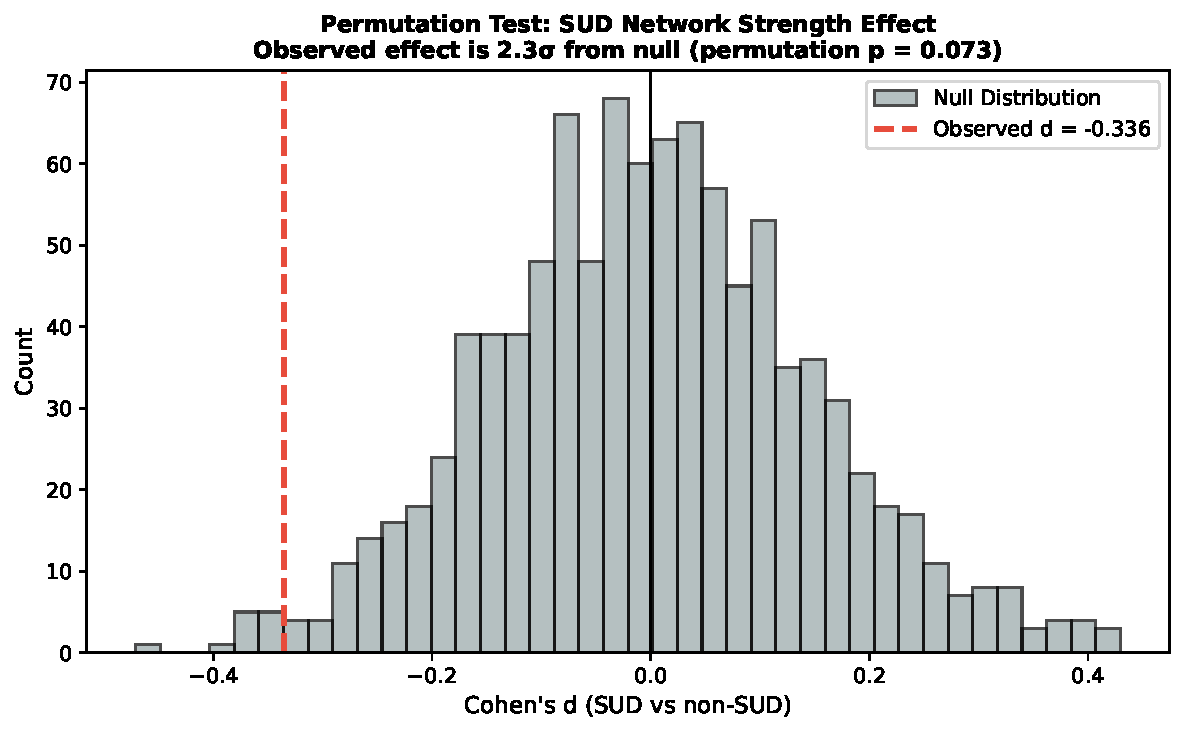
\includegraphics[width=0.55\textwidth]{pictures/chGraphNeuralNetworks/exp05_permutation_test.pdf}
    \caption{Permutation test for the SUD network strength effect. The observed effect (red dashed) is $2.3$ null standard deviations from the permutation mean, but the empirical permutation test does not reach significance ($p = 0.073$; $5{,}000$ permutations).}
    \label{fig:exp05_permutation}
\end{figure}

\begin{figure}[H]
    \centering
    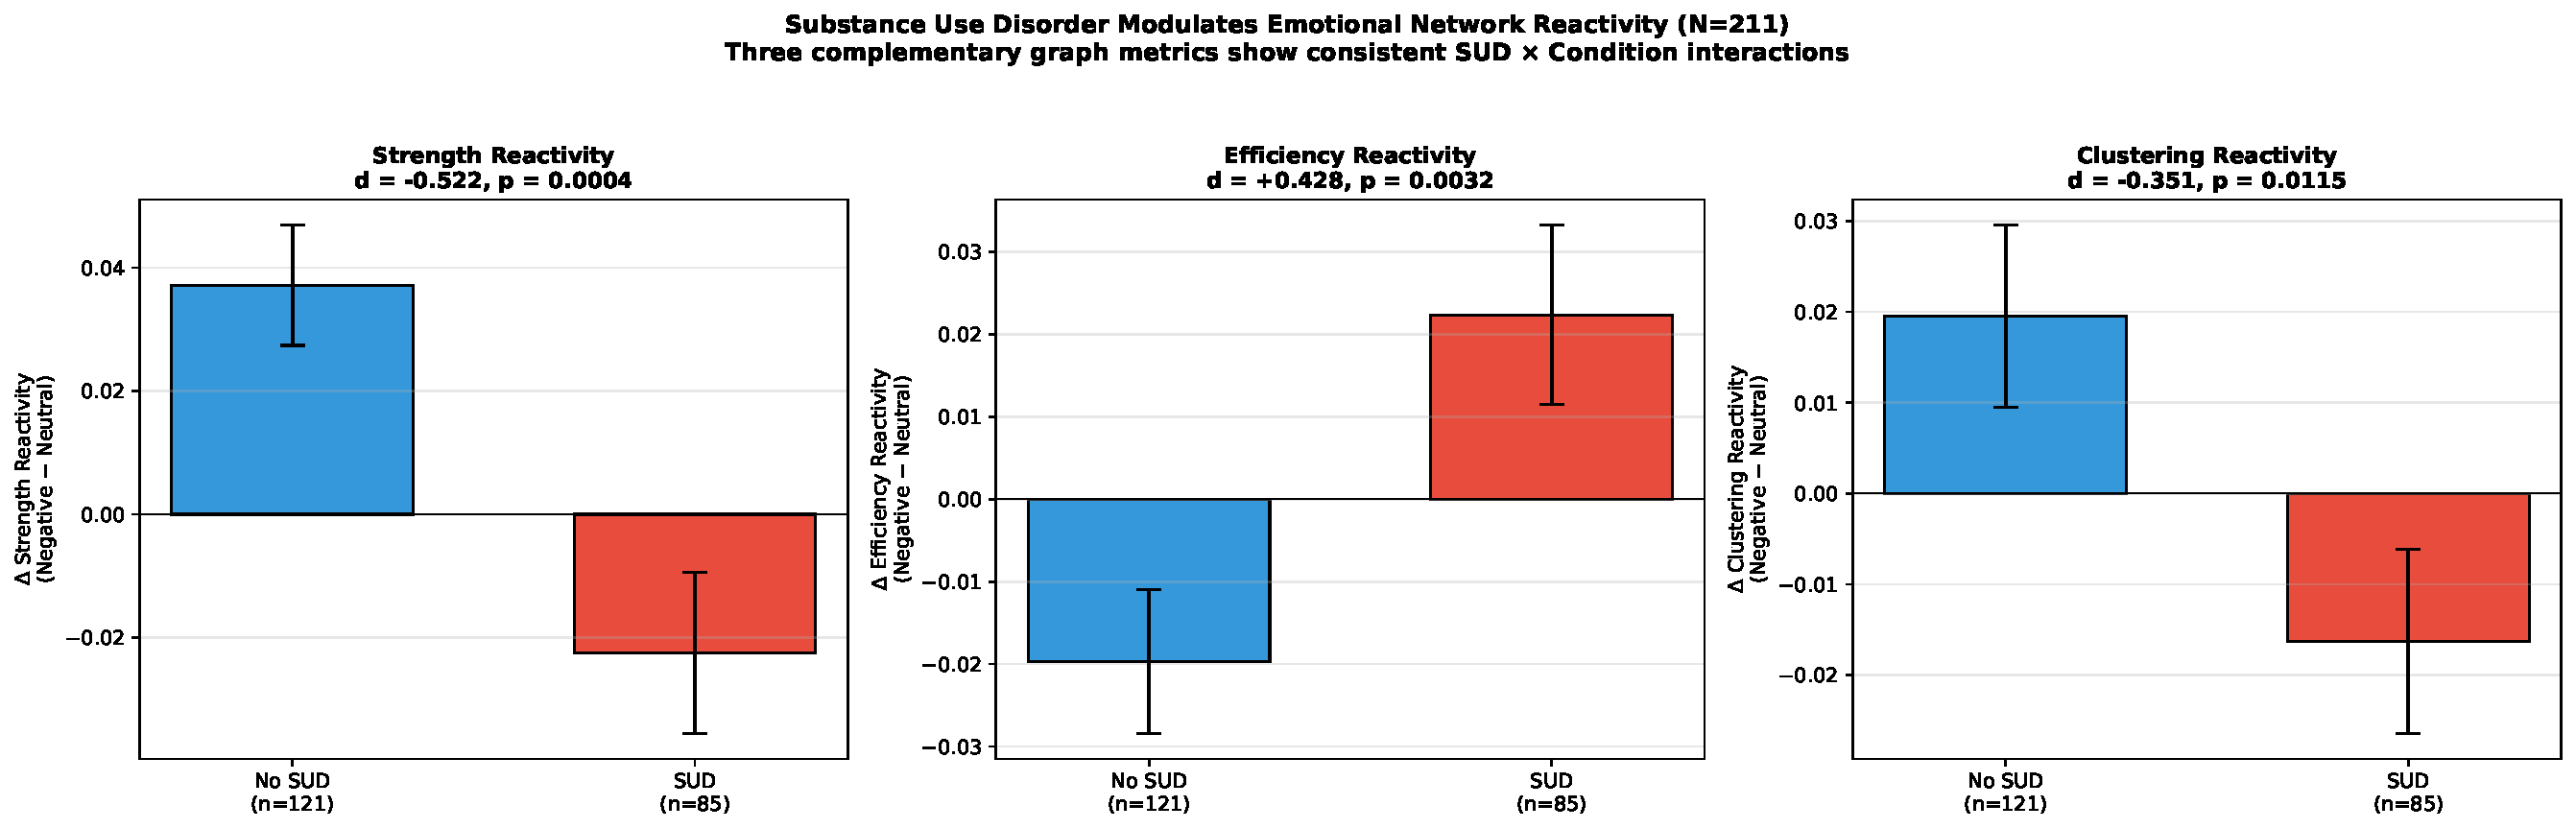
\includegraphics[width=\textwidth]{pictures/chGraphNeuralNetworks/fig_sud_interactions_211.pdf}
    \caption{Exploratory SUD reactivity comparisons for three archived graph summaries. The directions differ between groups; the strongest comparison has empirical permutation $p=0.073$. Error bars show SEM.}
    \label{fig:sud_interactions}
\end{figure}

\subsection{Additional Interaction Effects}

Two additional nominal interactions are GAD $\times$ efficiency reactivity ($d=-0.32$, $p=0.032$) and sex $\times$ strength reactivity ($d=+0.37$, $p=0.024$). Neither is multiplicity-adjusted, and six participants are absent from the binary sex counts; these comparisons are descriptive.

\subsection{Nested-Sample Stability Check}
\label{sec:ch5_nonrep}

Two nominal interactions from the initial $N=115$ subset were re-examined in the overlapping $N=211$ sample (Figure~\ref{fig:nonreplication}): medication $\times$ efficiency reactivity and PTSD $\times$ clustering reactivity. Neither has nominal $p<0.05$ in the larger sample. A change in significance does not itself establish that an effect is absent or sample-specific; effect estimates and uncertainty, not the dichotomy alone, should guide interpretation.

Because the samples overlap, this check is not an independent replication and cannot estimate reproducibility. It records how selected estimates changed when additional observations were added. All clinical-label findings require independent, prespecified evaluation with multiplicity control.

\begin{figure}[H]
    \centering
    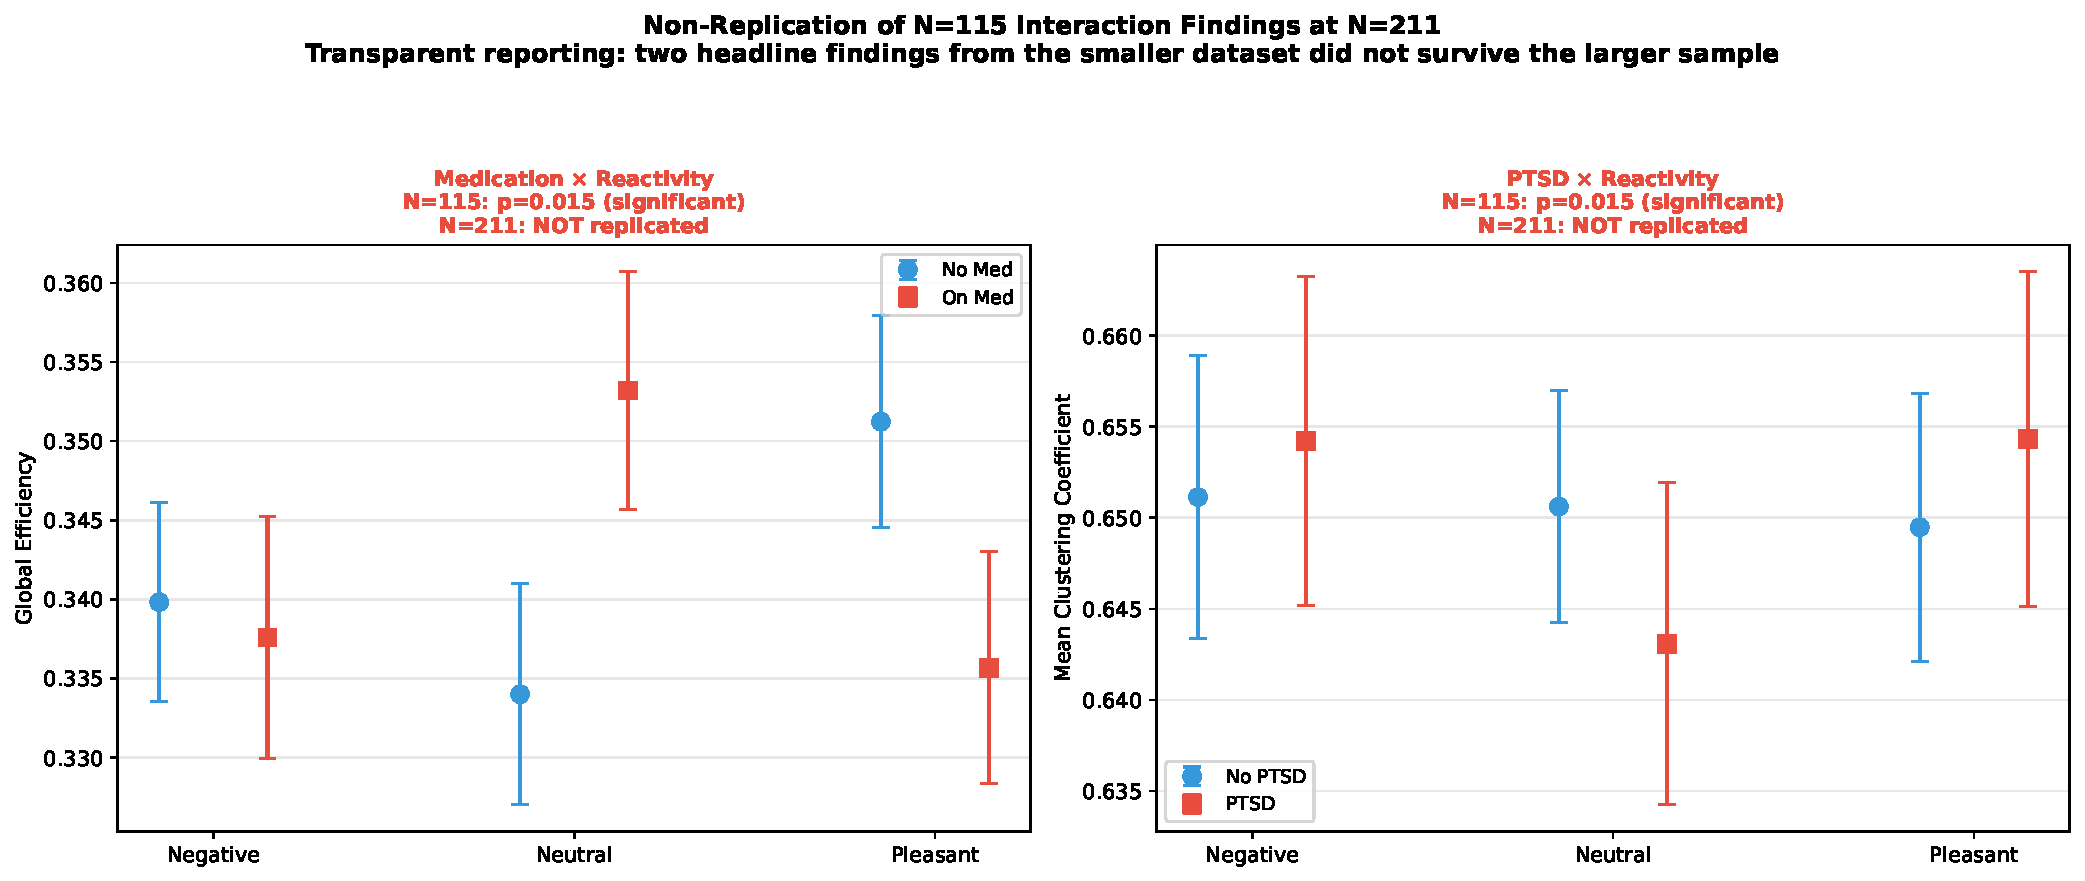
\includegraphics[width=\textwidth]{pictures/chGraphNeuralNetworks/fig_nonreplication_211.pdf}
    \caption{Nested-sample stability check for two exploratory interactions. The $N=115$ sample is contained within the $N=211$ sample, so this is not an independent replication.}
    \label{fig:nonreplication}
\end{figure}

\subsection{Edge-Level Comparisons}

No clinical variable produced edges surviving FDR correction (Figure~\ref{fig:edge_biomarkers}); the analysis therefore does not isolate any edge-level clinical association after multiplicity control. For PTSD, Ch0$\leftrightarrow$Ch27 is the strongest uncorrected single-edge effect ($d = +0.43$, $p = 0.003$), consistent with its ranking in the $N = 115$ analysis. Because the electrodes are unlabeled and the result does not survive FDR correction, anatomical or biomarker interpretation is not supported.

\begin{figure}[H]
    \centering
    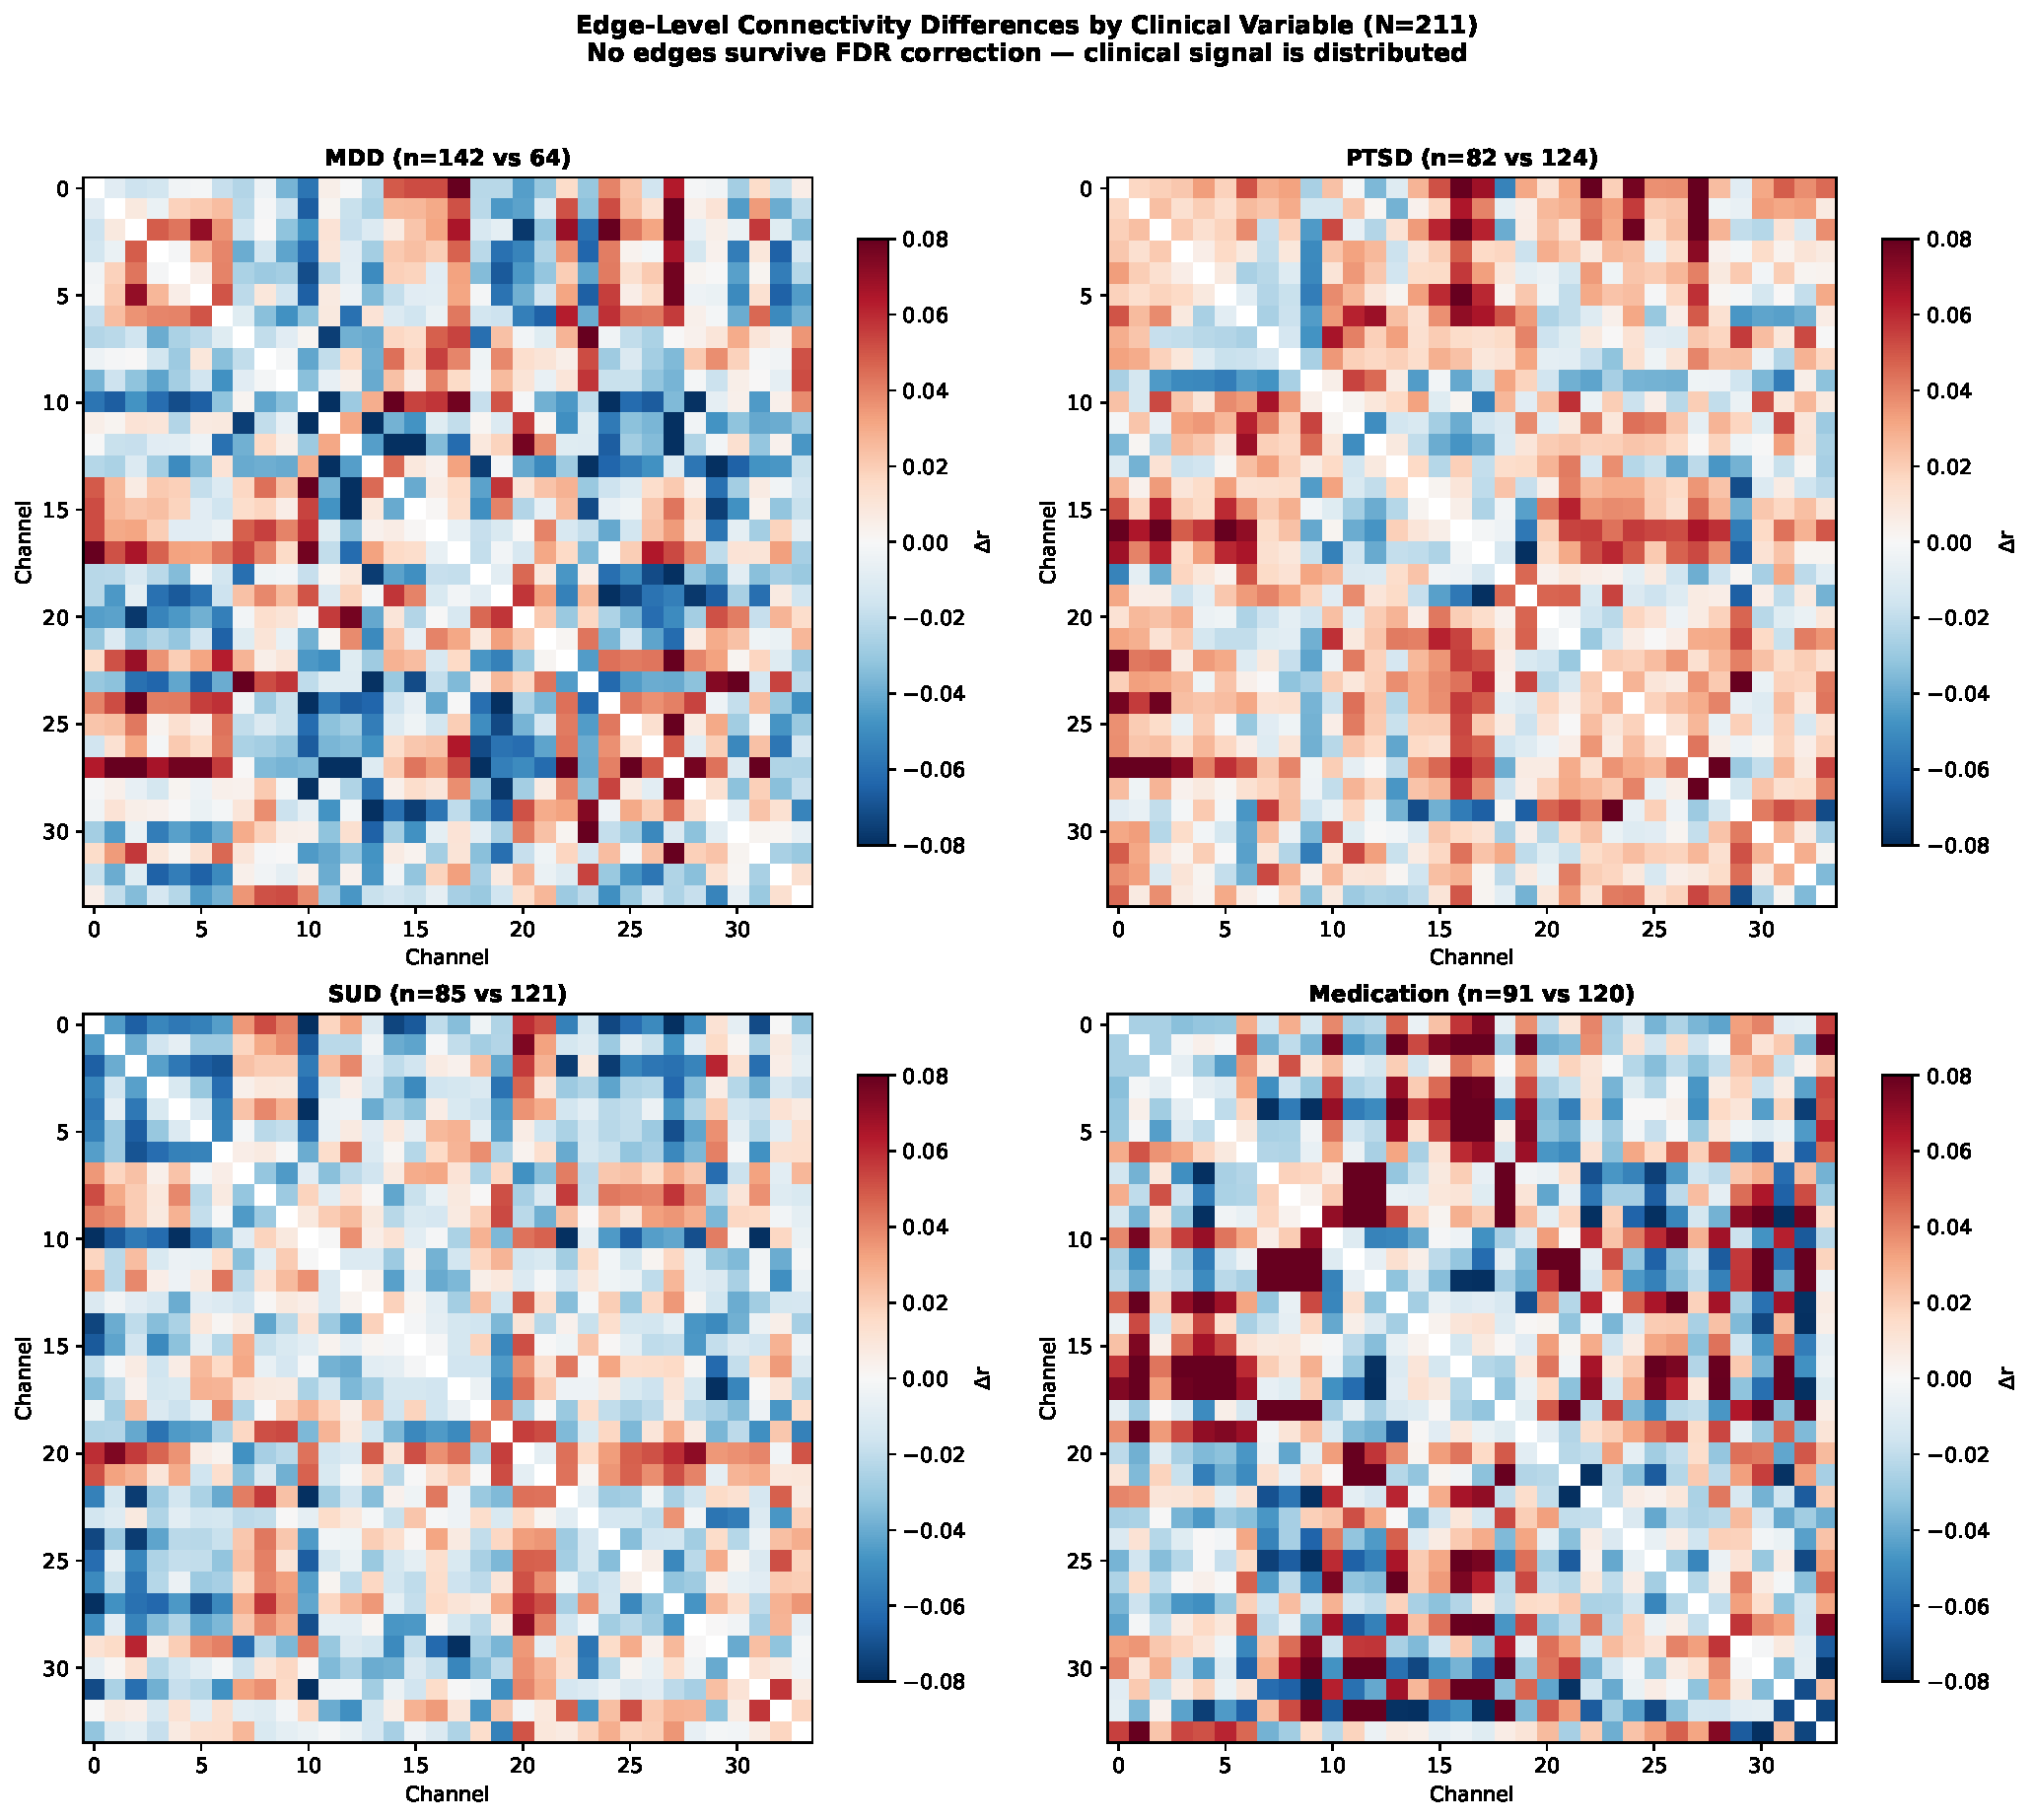
\includegraphics[width=\textwidth]{pictures/chGraphNeuralNetworks/fig_edge_biomarkers_211.pdf}
    \caption{Exploratory edge-level differences ($N=211$). No tested edge survives FDR correction.}
    \label{fig:edge_biomarkers}
\end{figure}


\section{Descriptive Comparison Across Label Granularities}
\label{sec:ch5_4class}

The archived project also analyzes four labels (Threat, Mutilation, Cute, and Erotic) for the same $211$ participants. The three- and four-class scripts do not implement a controlled one-factor comparison: they differ in the number of observations, class definitions, and details of PCA/feature processing. Both also use global PCA for the displayed results. The following numerical contrast is therefore descriptive and cannot isolate the causal effect of label granularity.

\subsection{Observed Performance Difference}

Table~\ref{tab:regime_comparison} records the displayed differences. In the three-class run, the reservoir estimate is $12.5$ percentage points above band-power; in the four-class run, it is $6.2$ points below band-power. Because the pipelines are not otherwise identical and preprocessing was not fold-safe, this reversal is a hypothesis to test, not an identified regime boundary.

\begin{table}[t]
\centering
\caption{Archived cross-granularity results. The runs differ in class structure and preprocessing details; values are descriptive and do not identify a causal regime transition.}
\label{tab:regime_comparison}
\small
\renewcommand{\arraystretch}{1.15}
\begin{tabular}{lcc}
\hline
\textbf{Quantity} & \textbf{3-class} & \textbf{4-class} \\
\hline
Number of classes & 3 & 4 \\
Best raw classifier & Reservoir + SVM & BandPower + SVM \\
Best raw balanced accuracy & $63.4\%$ & $40.4\%$ \\
Best centered accuracy & $79.4\%$ & $52.0\%$ \\
Subject-centering gain & $+16.0$ pp & $+10.8$ pp \\
Band-power accuracy & $50.9\%$ & $40.4\%$ \\
Reservoir $>$ BandPower? & Yes ($+12.5$ pp) & No ($-6.2$ pp) \\
GNN beats non-propagated? & No & No \\
Subject variance fraction & $62.6\%$ & $47.0\%$ \\
Condition variance fraction & $8.7\%$ & $2.4\%$ \\
Subject / condition ratio & $7.2\times$ & $19.6\times$ \\
Smallest nominal clinical $p$ & SUD $p = 0.0004$ & PTSD $p = 0.036$ \\
\hline
\end{tabular}
\end{table}

The archived variance decompositions assign $8.7\%$ to condition in the three-class representation and $2.4\%$ in the four-class representation. These decompositions were fitted to different design matrices and globally transformed feature spaces. They are compatible with weaker class separation in the four-class run, but they do not explain its cause or prove that temporal binning lacks the required resolution.

\subsection{Pairwise Accuracy Pattern}

In the archived pairwise results, Cute versus Erotic has the highest displayed accuracy ($69.0\%$), while Threat versus Cute has the lowest ($52.8\%$). An arousal account is plausible, but stimulus-level valence/arousal scores were not modeled here and the pairwise contrasts differ in more than one property. The result therefore does not establish that the reservoir is more sensitive to arousal than valence.

\subsection{Four-Class Clinical Findings}

In the four-class screen, PTSD has $11$ nominal channel--metric comparisons and $28$ nominal edge comparisons, and a PTSD $\times$ Threat--Mutilation term has nominal $p=0.036$. These counts and $p$ values are uncorrected. The SUD $\times$ global-efficiency term has nominal $p=0.008$, but a result from the same participants under a different labeling does not provide independent replication. Neither comparison supports a disorder signature.

The identity of the smallest nominal $p$ value differs across the two screens. Given the number of comparisons, overlapping sample, and pipeline differences, this ordering should not be interpreted as evidence that different disorders are detectable at different emotional resolutions.


\section{Layer Ablation and Complementarity Analysis}
\label{sec:ch5_ablation}

The preceding sections define an embedding block (E), a dynamical-summary block (D), a graph-summary block (T), and a coupling summary (C). This section compares their archived cross-validation estimates using $L_2$-regularized logistic regression. The comparison was not nested around all feature-selection and preprocessing decisions, so it is descriptive rather than a confirmatory test of complementarity.

\subsection{Emotion Classification Ablation}

Table~\ref{tab:emotion_ablation} presents the A1--A9 results on the three-class task. The largest displayed estimate is for the embedding-containing blocks, while topology and coupling are near chance. No nested model-comparison test or held-out selection procedure was used to establish differences among the close estimates. The table therefore ranks the archived point estimates but does not confirm that one block adds information beyond another.

\begin{table}[t]
\centering
\caption{Archived feature-block comparison for three-class classification (logistic regression, 10 subject-grouped folds). E~$=$~BSC$_6$/PCA-64 embedding; D~$=$~dynamical summaries; T~$=$~graph summaries; C~$=$~coupling scalar. PCA-dependent values use the earlier global-PCA pipeline.}
\label{tab:emotion_ablation}
\small
\begin{tabular}{llcc}
\hline
\textbf{ID} & \textbf{Features} & \textbf{Dim} & \textbf{Bal.\ Accuracy} \\
\hline
A0 & BandPower & 170 & $49.4 \pm 5.1\%$ \\
A1 & E & 2,176 & $59.4 \pm 3.6\%$ \\
A2 & D & 238 & $42.2 \pm 6.0\%$ \\
A3 & T & 68 & $35.3 \pm 4.7\%$ \\
A4 & C & 3 & $35.4 \pm 6.9\%$ \\
A5 & D + T & 306 & $43.8 \pm 7.2\%$ \\
A6 & E + D & 2,414 & $59.3 \pm 4.5\%$ \\
A7 & E + T & 2,244 & $60.1 \pm 4.3\%$ \\
A8 & E + D + T & 2,482 & $59.7 \pm 3.9\%$ \\
A9 & E + D + T + C & 2,485 & $59.4 \pm 3.8\%$ \\
\hline
\end{tabular}
\end{table}

In the RBF-SVM sensitivity run, E is $62.1\%$, D is $49.8\%$, and T shows no increase. This similar ordering is a descriptive sensitivity observation, not an independent confirmation.

\subsection{Clinical Detection Ablation}

The clinical-label estimates in Table~\ref{tab:clinical_ablation} range from $37.9\%$ to $53.8\%$ balanced accuracy and are mostly close to chance. The bold entries select the maximum within each diagnosis after observing the results; no nested selection, permutation test, or uncertainty interval establishes that those maxima differ from chance or from the other blocks. They should not be read as disorder-detection performance.

\begin{table}[t]
\centering
\caption{Exploratory clinical-label feature-block comparison (logistic regression, five subject-grouped folds). The maximum point estimate per label is bold; maxima were selected post hoc and do not establish layer-specific clinical sensitivity.}
\label{tab:clinical_ablation}
\small
\begin{tabular}{lccccc}
\hline
\textbf{ID} & \textbf{SUD} & \textbf{MDD} & \textbf{PTSD} & \textbf{GAD} & \textbf{ADHD} \\
\hline
C1 (E) & $50.9\%$ & $48.9\%$ & $45.2\%$ & $50.6\%$ & $52.8\%$ \\
C2 (D) & $\mathbf{53.6\%}$ & $44.6\%$ & $50.6\%$ & $50.2\%$ & $46.3\%$ \\
C3 (T) & $42.1\%$ & $48.6\%$ & $48.2\%$ & $51.1\%$ & $37.9\%$ \\
C4 (D+T) & $52.1\%$ & $43.9\%$ & $\mathbf{52.6\%}$ & $46.4\%$ & $46.4\%$ \\
C5 (E+D+T) & $48.5\%$ & $\mathbf{51.8\%}$ & $45.3\%$ & $50.0\%$ & $51.5\%$ \\
C6 (C) & $52.7\%$ & $49.7\%$ & $47.0\%$ & $\mathbf{53.8\%}$ & $\mathbf{53.0\%}$ \\
\hline
\end{tabular}
\end{table}

\subsection{Interpretation of the Feature Blocks}

For emotion labels, the embedding-containing blocks have the largest archived point estimates. For clinical labels, all maxima are weak and uncertain. The blocks are operationally different by construction because they summarize different quantities, but this ablation does not show that they carry unique clinical information or map to distinct disorder mechanisms.


\section{Engineering Interpretation}
\label{sec:ch5_novelty}

\subsection{Contributions and Limits}

This chapter documents class-geometry summaries, propagation sweeps, a subject-panel normalization analysis, a cross-granularity comparison, and feature-block ablations. The post-defense audit identified global PCA and incompatible per-channel PCA bases in the archived Chapter~5 workflow. Consequently, results that depend on those operations are preserved for transparency as descriptive legacy estimates. The clinical-label analyses are exploratory, and the strongest SUD permutation result is $p=0.073$.

\subsection{Significance for Electrical Engineering}

The Propagation Operating Characteristic provides a systematic way to compare graph operators on finite sensor arrays. Across the tested GCN, high-pass, residual, difference-aware, self-attention, and no-propagation variants, the non-propagated representation yields the strongest measured separability. The subject--condition shared-subspace result also cautions against assuming that PCA-based nuisance removal is lossless. The node-count and density thresholds observed here are hypotheses for other EEG and biosignal graphs, not general design laws for ECG, EMG, or fNIRS.

\subsection{Clinical Interpretation Limits}

The clinical screens suggest questions for a future study but do not support clinical electrophysiology conclusions. The graph quantities are derived from reservoir features, not direct measurements of brain-network connectivity; montage labels are unavailable; the strongest SUD comparison fails its permutation test; and the analysis does not show an advantage over a multiplicity-controlled spectral-feature alternative.

The panel-centering result illustrates that repeated observations from a held-out subject can be used to remove that subject's mean feature vector. It does not demonstrate a field-wide flaw or show that a biological ``subject-identity component'' has been isolated. Its relevance is limited to designs in which all required within-subject observations are available together.


\section{Scope and Future Directions}
\label{sec:ch5_scope}

Future work should begin with verified electrode labels and montage coordinates, fold-local common-basis dimensionality reduction, nested model selection, and a prespecified multiplicity plan. The corrected pipeline should be rerun on the raw SHAPE data and tested in an independent cohort before clinical interpretation. Longitudinal data would also be required to distinguish stable participant differences from session and condition effects.


\section{Empirical Investigation of Traceability}
\label{sec:ch5_interpretability_investigation}

This section examines which intermediate quantities can be inspected and related to predefined temporal windows. Inspectability is not equated with faithful causal explanation, clinical usefulness, or model correctness.

\subsection{Theoretical Context: Interpretability in Spiking Neural Networks}
\label{sec:interp_theory}

Spiking models expose discrete event traces, but those traces are not self-interpreting. Anatomically structured systems such as NeuCube can associate learned activity with supplied coordinates \cite{kasabov_neucube_2014,doborjeh_explainable_2021}, and attention mechanisms can provide temporal weights \cite{yao_attention_snn_2023}. In each case, fidelity and usefulness require empirical evaluation; the presence of spikes, coordinates, or attention weights alone does not establish an explanation \cite{kim_sam_2021}.

Published approaches include spike-based activation maps, prototype explanations, readout-weight analyses, and dynamical summaries \cite{kim_sam_2021,barnett_protopmed_2024,alao_discovering_2021,reservoir_pe_2022}. These methods answer different questions, and no result in this dissertation establishes that the present pipeline is more interpretable than a non-spiking alternative.

The present investigation therefore tests limited forms of temporal indexing and case-based summarization while recording their inferential limits.

\subsection{Archived PCA and Centering Result}
\label{sec:shared_subspace}

In the archived global-PCA representation, the tested linear models do not recover the selected ERP scalars after panel centering ($R^2\leq-0.04$), and the tested classifiers are near chance. This is a negative result for those transformations and models, not evidence that the representation contains no recoverable condition information.

The archived subspace calculation reports first-five principal angles of $0^\circ$. Exact zero angles in a globally fitted, high-dimensional sample representation can arise from shared or saturated sample subspaces and do not show that the underlying population effects are identical. Panel centering subtracts each subject's across-condition mean; it is not a projection that necessarily removes every condition contrast.

The negative result motivates examining pre-compression temporal features and rerunning PCA within each training fold. It does not identify PCA as the unique cause of lost traceability, because the archived comparison changes several operations and does not perform a causal ablation.

\subsection{Aggregate Associations with ERP Summaries}
\label{sec:erp_recovery}

This supplementary analysis uses a separate early-window extractor spanning $39$ to $273$~ms; it is not the archived full-epoch embedding used in the primary Chapter~5 tables. Its aggregate correlations with broader P300 ($250$--$500$~ms) and LPP ($500$--$800$~ms) scalar summaries are $r=0.65$ and $|r|=0.82$, respectively; the early-window BSC$_6$ spike-count correlations are $r=0.33$ and $|r|=0.23$. Because most of the P300 window and the entire LPP window lie outside the six-bin span, these correlations cannot be interpreted as recovery or temporal localization of those components. They are aggregate cohort associations whose computation requires independent verification.

A separate sweep compares three binning resolutions:
\begin{center}
\begin{tabular}{lcccc}
\toprule
\textbf{Bins} & \textbf{Resolution} & \textbf{Accuracy} & \textbf{Peak Bin} & \textbf{Concentration} \\
\midrule
6 & 39.1~ms & $67.0\% \pm 5.4\%$ & Bin 6 (234--273~ms) & 1.039 \\
12 & 19.5~ms & $65.9\% \pm 3.3\%$ & Bin 10 (176--195~ms) & 1.057 \\
24 & 7.8~ms & $63.5\% \pm 5.5\%$ & Bin 22 (172--180~ms) & 1.047 \\
\bottomrule
\end{tabular}
\end{center}
The displayed accuracy decreases as the number of bins increases. This may reflect dimensionality, regularization, or sampling variability. Mutual information was not estimated, so the result does not establish an information-bottleneck frontier or show that the added dimensions are purely nuisance.

The selected peak shifts from 234--273~ms at six-bin resolution to intervals near 176--195~ms at finer resolutions. These data-driven bin labels are not component measurements and are not assigned P300, LPP, or N2 interpretations.

\subsection{Temporal-Attention and Prototype Readout}
\label{sec:interpretable_readout}

Motivated by the direct indexing of predefined temporal bins, and by prototype-based EEG explanations \cite{barnett_protopmed_2024}, the logistic-regression comparison is augmented with attention and prototype modules operating on panel-centered temporal-bin features.

\paragraph{Architecture.} A lightweight LIF layer ($H = 32$ hidden units, fixed random input weights, learnable threshold $\theta$) processes the six temporal bins as a spike-driven sequence. Temporal attention ($\boldsymbol{\alpha} \in \Delta^5$) and channel attention ($\boldsymbol{\beta} \in \Delta^{33}$) produce importance weights via learned scoring functions with softmax normalization. The attended representation is classified by cosine similarity to $K = 5$ learned prototypes per class ($15$ total), with a learnable temperature $\tau$. Training uses cross-entropy loss with Adam optimization and early stopping under the same $10$-fold StratifiedGroupKFold protocol.

\paragraph{Classification Accuracy.} The interpretable readout was evaluated on two feature sets: centered raw EEG temporal bins (per-channel mean amplitude in six BSC$_6$-aligned windows) and centered BSC$_6$ spike counts produced by the actual LIF reservoir with recurrent connections (spectral radius $= 0.9$, $256$ neurons, $\approx 104{,}000$ spikes per observation, $7.2\%$ sparsity).

On raw EEG temporal bins, the readout achieves $66.7\% \pm 6.3\%$ balanced accuracy, compared with $67.1\% \pm 5.3\%$ for logistic regression on the same features. On BSC$_6$ spike features, the estimates are $57.5\% \pm 5.7\%$ and $56.1\% \pm 6.0\%$, respectively. The difference between raw and spike-bin results is compatible with information changing under the nonlinear reservoir transformation, but it does not show that the resulting space is optimized for temporal integration or identify why accuracy differs.

In the condition averages after reservoir transformation, Negative peaks in the final temporal bin ($\alpha = 0.177$), Neutral in the fifth ($\alpha = 0.176$), and Pleasant in the fourth ($\alpha = 0.180$). The profiles on raw EEG bins have a smaller displayed range. These are descriptive averages, not evidence of condition separation at the individual-observation level; the permutation test below yields $p = 0.634$.

\paragraph{Condition-Averaged Temporal Attention Profiles.} On raw EEG bins, Negative and Neutral stimuli produce peak attention in the first window (39--78~ms, $\alpha = 0.182$ and $0.179$), while Pleasant stimuli peak in the final window (234--273~ms, $\alpha = 0.175$). On BSC$_6$ spike features from the reservoir, Negative peaks in the final bin ($\alpha = 0.177$), Neutral in the fifth bin ($\alpha = 0.176$), and Pleasant in the fourth bin ($\alpha = 0.180$). These temporal labels indicate bin correspondence, not recovery of physiological ERP components. The inferential tests below do not support condition-specific attention separation.

An information-theoretic analysis quantifies attention concentration. The mean temporal attention entropy is $1.630$ nats versus $1.792$ for the uniform distribution, a $9.0\%$ entropy reduction. This indicates modest temporal concentration. Pleasant stimuli show the largest descriptive concentration ($9.4\%$ reduction).

A permutation test ($10{,}000$ shuffles of condition labels) evaluates whether the condition-specific attention profiles are statistically distinguishable. The observed sum-of-peak-attention statistic does not reach significance ($p = 0.634$), and per-bin Kruskal--Wallis tests across conditions yield $p > 0.48$ for all six bins. The per-sample attention distributions overlap substantially. The condition-average trends reported above are therefore descriptive and do not survive inference at the per-sample level. The attention readout provides temporal indexing at the population-average level but does not establish condition-specific resolving power at the individual-observation level.

\paragraph{Classification Confusion Structure.} In the archived confusion matrix for the raw-EEG attention--prototype readout, Neutral has $89\%$ recall and Negative has $49\%$ recall, with $35\%$ of Negative observations classified as Pleasant. An arousal account is possible but was not directly tested. Moreover, the lower Negative--Pleasant same-prototype rate ($28\%$) than the corresponding Neutral pairings ($33$--$35\%$) indicates greater prototype separation, not greater overlap; the two summaries therefore should not be presented as mutually confirming evidence.

\paragraph{Channel Attention Is Near-Uniform.} Channel-attention entropy is $3.524$ nats, compared with $3.526$ for uniform weights. This small difference provides no evidence of selective channel weighting. Panel centering may alter available channel structure, and the SHAPE files use unlabeled channel indices, so the weights also lack anatomical interpretation. The experiment does not validate the channel-attention module as a spatial explanation mechanism. NeuCube \cite{kasabov_neucube_2014}, by comparison, uses supplied coordinates to organize its model.

\paragraph{Prototype Assignments Provide Case-Based Summaries.} Ten of fifteen prototypes have archived classification purity above $60\%$, with one Neutral prototype reaching $93\%$. These are data-dependent cohort summaries. The reported cross-assignment statistics are not internally sufficient to establish an arousal interpretation, and calibration for individual decisions was not evaluated.

\paragraph{The LIF Threshold Is Inspectable.} Across folds, the fitted threshold is approximately $\theta=0.32$ (initialized at $0.50$). The scalar has a clear role in the model, but the readout also learns two attention networks, fifteen prototype vectors, and a temperature. Inspecting the threshold therefore does not make the entire learned component transparent or give it a direct biological interpretation.

\subsection{Interpretation of the Traceability Analysis}
\label{sec:interp_synthesis}

The five-stage investigation produces a structured characterization of where ARSPI-Net's interpretability resides and where it does not.

\paragraph{The pipeline exposes two kinds of summaries.} Pre-reservoir bins provide directly indexed early time windows, while post-reservoir BSC$_6$ features summarize spike counts. Their archived aggregate correlations with ERP scalars are reported above but do not temporally recover components outside the bin span. The attention profiles do not survive permutation testing, so the supported claim is limited to inspectability of predefined bins.

\paragraph{The archived PCA representation has limited traceability.} The tested centered PCA-64 features do not predict the selected ERP scalars. Fold-local PCA and alternative compression methods should be evaluated before attributing the result to a structural property of the SHAPE data.

\paragraph{The attention readout provides temporal indexing.} The learned attention can be mapped to six predefined temporal bins. The $9\%$ entropy reduction is modest, and the condition-average profiles do not survive permutation testing ($p = 0.634$). The measurement therefore supports inspectable temporal weighting without establishing condition-specific attention separation.

\paragraph{Prototype purity is descriptive.} The prototype-purity values range from $53\%$ to $93\%$ in this cohort. They were not calibrated as confidence scores, and prospective reliability and clinician use were not tested.

\paragraph{Audit summary.} The archived variance decomposition, panel-centering changes, zero principal-angle calculation, attention readout, and prototype assignments describe different aspects of the same cohort. Global preprocessing and the transductive panel estimand limit the geometric results. The attention profiles are not condition-separable under the reported permutation test, and the prototypes lack external calibration. The supported contribution is the ability to inspect these calculations, not validation of a clinical explanation chain.

\paragraph{What remains to be tested.} A future study could use verified electrode labels, independent data, and prespecified fidelity tests for channel attention. Projecting prototypes back to waveform space would allow comparison with defined ERP summaries. Gradient attribution for spikes \cite{bitar_snn_grad_2023} and Spike Activation Maps \cite{kim_sam_2021} are candidate methods for a broader comparison.

\subsection{Head-to-Head: EEGNet Saliency vs.\ ARSPI-Net Attention}
\label{sec:shap_comparison}

The preceding sections show that ARSPI-Net's attention readout produces temporally indexed condition averages, although those profiles are not statistically separable by condition. This subsection compares those weights with post-hoc input--gradient products from EEGNet. The centered EEGNet estimate is $86.3\%\pm4.0\%$ balanced accuracy under the transductive panel normalization used in this experiment.\footnote{Table~\ref{tab:conventional_baselines} reports $89.1\%$ for EEGNet with a different training schedule. The saliency run uses 150 epochs and a fixed learning-rate schedule rather than 200 epochs with ReduceLROnPlateau. The values are therefore not a controlled estimate of a 2.8 percentage-point training effect.}

\paragraph{Method.} EEGNet \cite{lawhern_eegnet_2018} was trained on panel-centered SHAPE data under the same grouped-fold protocol. Input--gradient products \cite{shrikumar_deeplift_2017} were computed for each test observation and output class, producing attribution values at 256 time steps ($3.9$~ms each). Absolute values were averaged across channels and observations within condition. They were then binned into the six BSC$_6$-aligned windows (39--273~ms) and normalized to align their time scale with the attention display; the two attribution quantities are not otherwise equivalent.

\paragraph{EEGNet's unbinned saliency peaks later than the BSC$_6$ attention span.} The temporal saliency maxima occur at $691$~ms for Negative, $441$~ms for Neutral, and $402$~ms for Pleasant. The $691$~ms maximum lies within the dissertation's stated $500$--$800$~ms LPP interval; the other two lie in the broader late-positive interval before $500$~ms. All three occur later than the $39$--$273$~ms span represented by the six ARSPI-Net attention bins. These model-dependent maxima do not identify physiological component generators.

\paragraph{ARSPI-Net attention peaks within predefined early post-stimulus bins.} ARSPI-Net's condition-average BSC$_6$ attention peaks at $254$~ms for Negative, $214$~ms for Neutral, and $176$~ms for Pleasant. Each value maps directly to a predefined time bin. Because the condition-profile permutation test yields $p = 0.634$, the peaks do not establish distinct temporal strategies or identify a physiological ERP component as the cause of an individual prediction.

\paragraph{Quantitative comparison.} The binned saliency and ARSPI-Net attention show weak correlation (Negative: $r = -0.36$; Neutral: $r = -0.05$; Pleasant: $r = 0.18$ for raw attention), indicating that the two methods assign weight to different temporal regions. EEGNet's binned saliency peaks in the final BSC$_6$ bin for Negative ($0.198$) and Neutral ($0.228$) and in an earlier bin for Pleasant ($0.203$), partially overlapping the ARSPI-Net profile. Saliency attribution entropy ($H = 1.770$--$1.783$) is marginally lower than ARSPI-Net attention entropy ($H = 1.791$), so EEGNet is slightly more concentrated by this metric.

\begin{figure}[t]
\centering
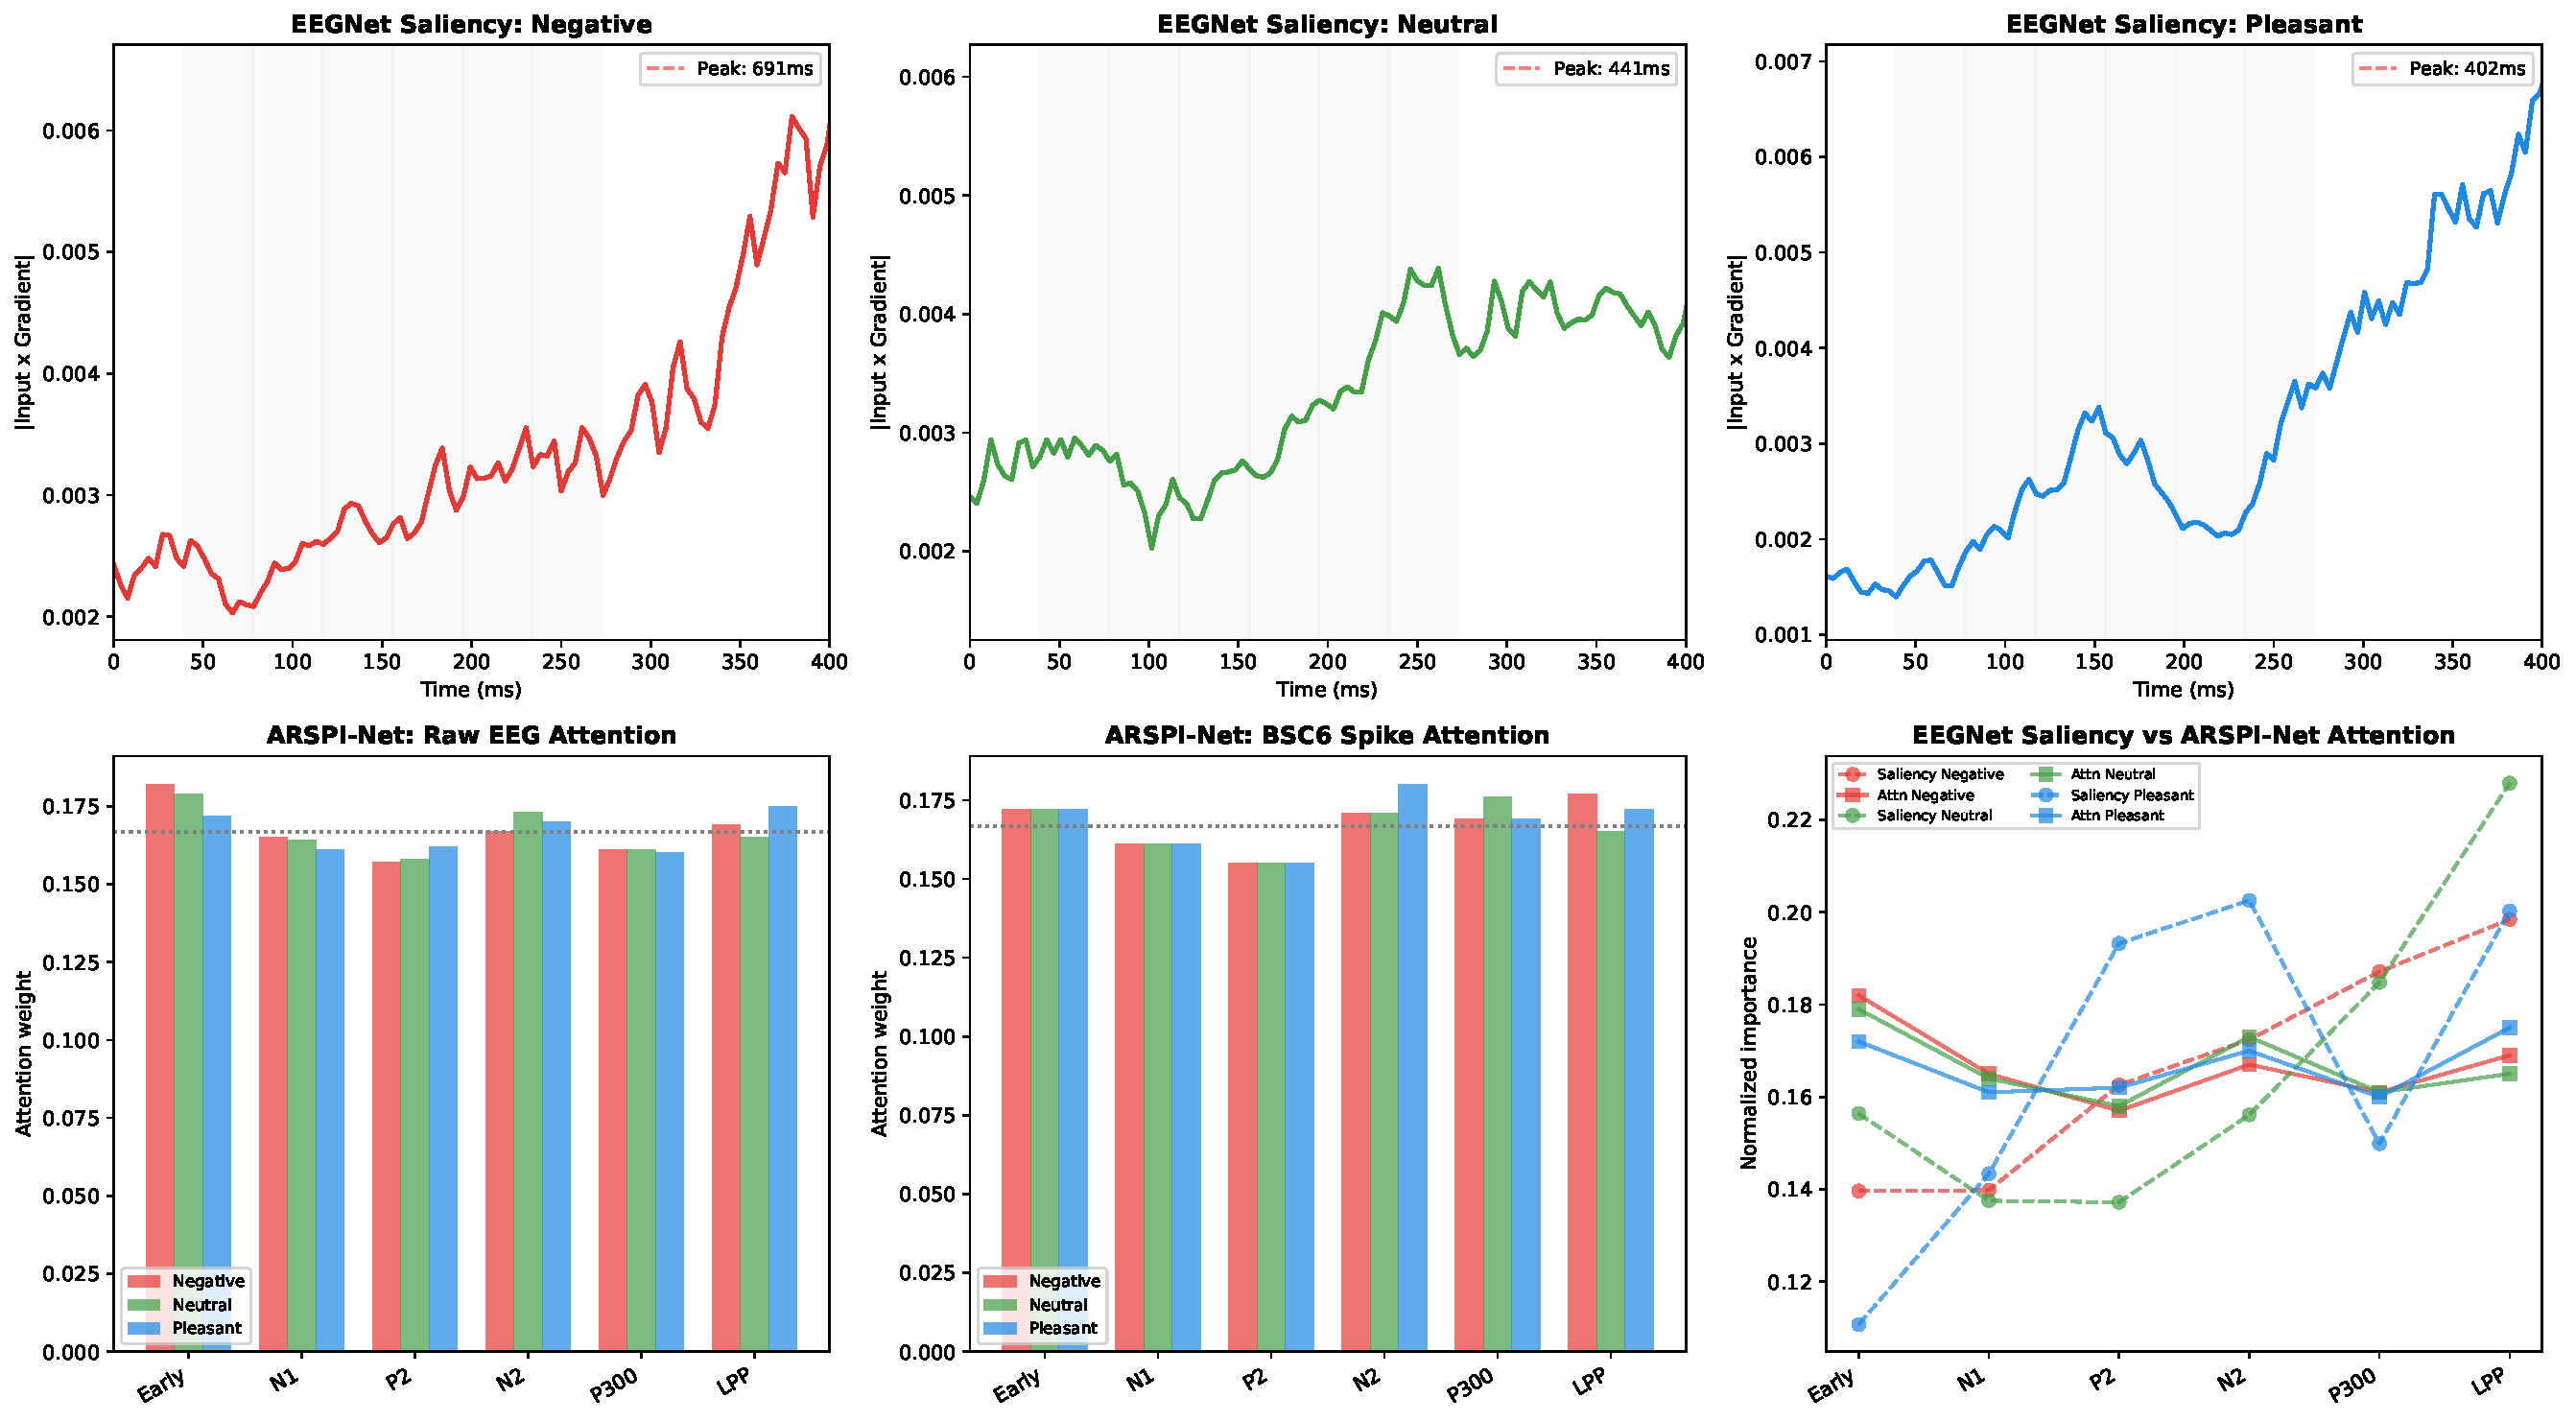
\includegraphics[width=\textwidth]{pictures/chGraphNeuralNetworks/fig_shap_comparison.pdf}
\caption[Temporal attribution summaries for EEGNet and ARSPI-Net.]{Temporal attribution summaries for EEGNet (input--gradient products, top row) and ARSPI-Net (learned attention weights, bottom left and center). EEGNet's unbinned maxima occur at $691$~ms (Negative), $441$~ms (Neutral), and $402$~ms (Pleasant). The bottom-right panel aligns both displays to the same six early intervals. The ARSPI-Net condition-profile permutation test gives $p=0.634$.}
\label{fig:shap_comparison}
\end{figure}

\paragraph{Interpretation.} Both quantities are model-dependent attribution summaries. The input--gradient product is post hoc, while ARSPI-Net attention is learned on predefined temporal bins. Mapping a weight to a bin improves traceability, but does not establish causal fidelity or exclude nuisance structure. Accuracy differences cannot be interpreted as the cost of interpretability because the model classes and training procedures differ. The two displays assign weight to different temporal regions under these fitted models.




\section{Connection to Dynamical Analysis}
\label{sec:ch5_bridge}

This chapter characterizes the archived embedding and graph-summary blocks. The feature-block analysis shows the largest emotion-label point estimates for embedding-containing models, while clinical-label estimates remain near chance and do not establish disorder detection. Chapter~\ref{chap:dynamics} describes reservoir-trajectory summaries, and Chapter~\ref{chap:synthesis} examines their descriptive association with graph summaries across channel indices.


\section{Chapter Summary}
\label{sec:ch5_summary}

This chapter reports analyses of $211$ participants ($633$ observations in the three-class data and $844$ in the four-class data). The post-defense audit changes the status of several results: PCA-dependent and incompatible-basis graph values are descriptive legacy estimates pending rerun with raw SHAPE data.

First, the archived variance decomposition assigns more variation to participants than conditions. Panel centering increases the displayed estimates across the tested representations, but it uses all three held-out observations for each subject and is not a prospective single-observation estimate.

Second, none of the tested propagation operators exceeds the non-propagated comparison in the archived sweep. This result is configuration- and cohort-specific.

Third, removing leading global-PCA components reduces the archived accuracy. The analysis does not prove that subject and condition effects occupy identical population subspaces.

Fourth, the exploratory clinical screen contains nominal SUD comparisons, but the strongest label-permutation check yields $p=0.073$, edge results do not survive FDR correction, and the nested-sample check is not an independent replication.

Fifth, the three- and four-class runs show different point-estimate rankings, but pipeline differences and global preprocessing confound the comparison; no regime transition or disorder hierarchy is established.

Sixth, embedding-containing models have the largest archived emotion-label point estimates in the feature-block comparison. A fold-safe rerun and nested comparison are needed before making an incremental-information claim.

Seventh, the clinical-label block estimates are mostly near chance, and post-hoc maxima do not establish layer-specific clinical sensitivity.

Finally, the baseline table records archived point estimates for several models. Differences in training protocols, global preprocessing, and the transductive panel-centering estimand prevent a definitive architecture ranking or a claim of intrinsic interpretability.
